\documentclass[aspectratio=169]{beamer}

\usepackage{lmodern,graphicx,amsthm,amsmath,amssymb,braket}
\usepackage[absolute,overlay]{textpos}

\usetheme{focus}

\usepackage[backend=bibtex,url=false,doi=false,style=authoryear]{biblatex}
\bibliography{kondo_presentation}
\AtBeginBibliography{\scriptsize}

\newcommand{\head}[1]{
\begin{textblock*}{\textwidth}(20pt, 40pt)
\textbf{\Large {#1}}
\end{textblock*}
}
\newcommand{\focus}[1]{\textcolor{maroon}{\textbf{#1}}}
\renewcommand{\thefootnote}{}
\renewcommand*\footnoterule{}

\definecolor{maroon}{HTML}{540000}
\definecolor{lblue}{HTML}{8888ff}
\definecolor{lyellow}{HTML}{ffcc99}
\setbeamercolor{footnote}{fg=blue}
\setbeamerfont{footnote}{size=\small}
\setbeamertemplate{bibliography item}[triangle]

\AtBeginSection[]{
\begin{frame}[noframenumbering]
  \vfill
  \centering
  \begin{beamercolorbox}[sep=8pt,center,rounded=true]{title}
    \usebeamerfont{title}\insertsectionhead\par%
  \end{beamercolorbox}
  \vfill
\end{frame}
}

\title{
\LARGE{Unveiling the Kondo cloud: \\
unitary RG study of the Kondo\\
model%
}
}
\subtitle{\bf\large\color{lyellow}\href{https://arxiv.org/abs/2111.10580}{arXiv:2111.10580v2[cond-mat.str-el]}}
\date{\today}
\author{\large Anirban Mukherjee \inst{1}, Abhirup Mukherjee \inst{1}, N. S. Vidhyadhiraja \inst{2},\\ A. Taraphder \inst{3}, Siddhartha Lal \inst{1}}


\institute{\small\inst{1} Department of Physical Sciences,IISER Kolkata, ~ ~ \inst{2} Theoretical Sciences Unit, JNCASR, ~ ~ \inst{3} Department of Physics, IIT Kharagpur}
\date{\large\today}

\begin{document}

\begin{frame}[noframenumbering]
\maketitle
\begin{textblock*}{0.45\textwidth}(9.4cm, 0.7cm)
	\centering
	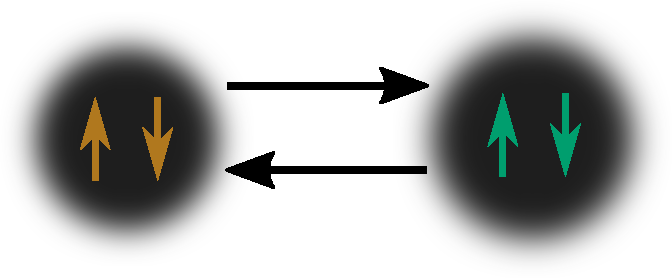
\includegraphics[width=\textwidth]{figures/kondo_zeromode_banner.pdf}
\end{textblock*}
\begin{textblock*}{0.7\textwidth}(5.5cm, 6.5cm)
	\centering
	
\includegraphics[width=0.15\textwidth]{figures/epqm_logo_mod.jpeg}
	\hspace*{\fill}
	
\includegraphics[width=0.15\textwidth]{figures/dps_logo.jpeg}
	\hspace*{\fill}
	
\includegraphics[width=0.15\textwidth]{figures/jncasr_logo.pdf}
	\hspace*{\fill}
	
\includegraphics[width=0.15\textwidth]{figures/kgp_logo.pdf}
\end{textblock*}
\end{frame}

\section{The Model}
\begin{frame}[noframenumbering]{The Model}
\only<+>{\centering
	\[H = \sum_{k\sigma}\epsilon_k \hat n_{k\sigma} + J \vec{S}_d\cdot\vec{s}, ~ ~ ~ ~ ~ \vec s \equiv \sum_{kk^\prime,\alpha,\beta}\vec \sigma_{\alpha\beta}c^\dagger_{k\alpha}c_{k^\prime\beta}, ~ ~ ~ ~ ~\vec S_d \longrightarrow\text{impurity spin}\]
	\focus{local \(s-\)wave interaction} between impurity spin \(\vec S_d\) and conduction electrons \(\vec s\)

\begin{figure}
\hspace*{\fill}
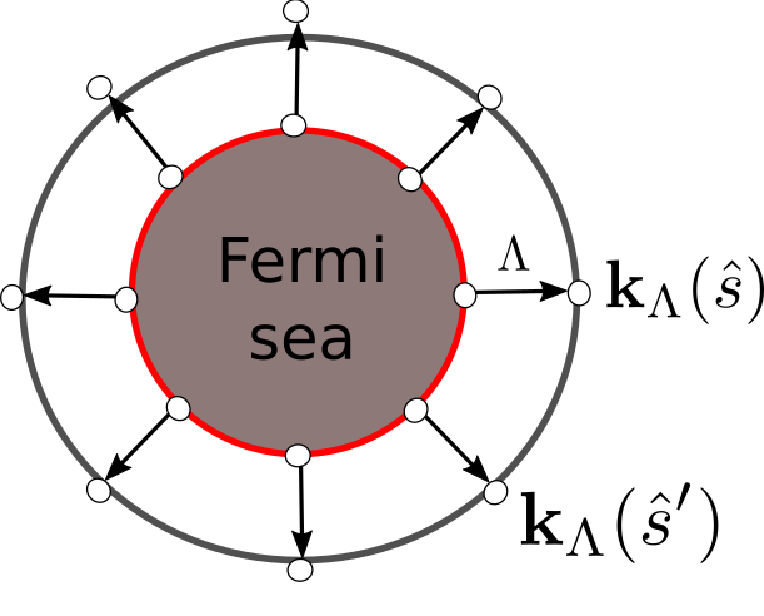
\includegraphics[width=0.3\textwidth]{figures/2dKondoTN.pdf}
\hspace*{\fill}
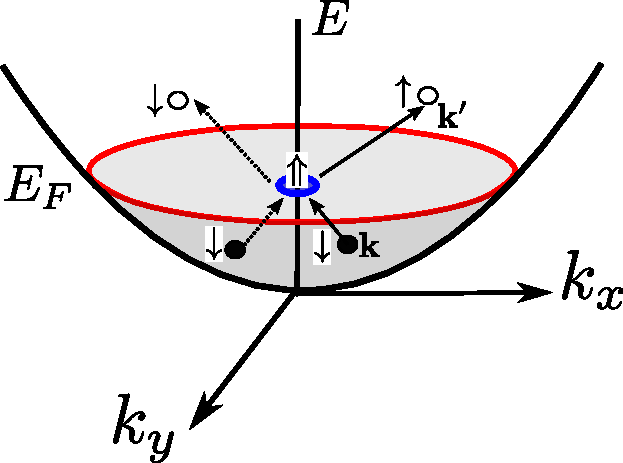
\includegraphics[width=0.3\textwidth]{figures/kondoSetup.pdf}
\hspace*{\fill}
\end{figure}
\begin{textblock*}{0.45\textwidth}(9.4cm, 0.85\textheight)
	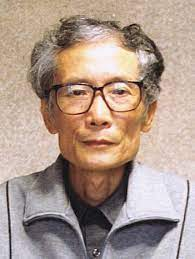
\includegraphics[height=40pt]{figures/kondo.jpeg}
\end{textblock*}
\footcite{kondo1964resistance,Schrieffer_Wolff}
}
\only<2-5>{
\begin{minipage}{0.6\textwidth}
\begin{itemize}[<+-|alert@+>]
\item Kondo coupling \(J\) renormalises to infinity\\[10pt]
\item low energy phase of metal is local Fermi liquid\\[10pt]
\item \(\chi\) constant at low temperatures, \(C_v\) linear\\[10pt]
\item thermal quantities functions of single scale \(T/T_K\)\\[10pt]
\end{itemize}
\end{minipage}
\begin{minipage}{0.35\textwidth}
	\only<2-3>{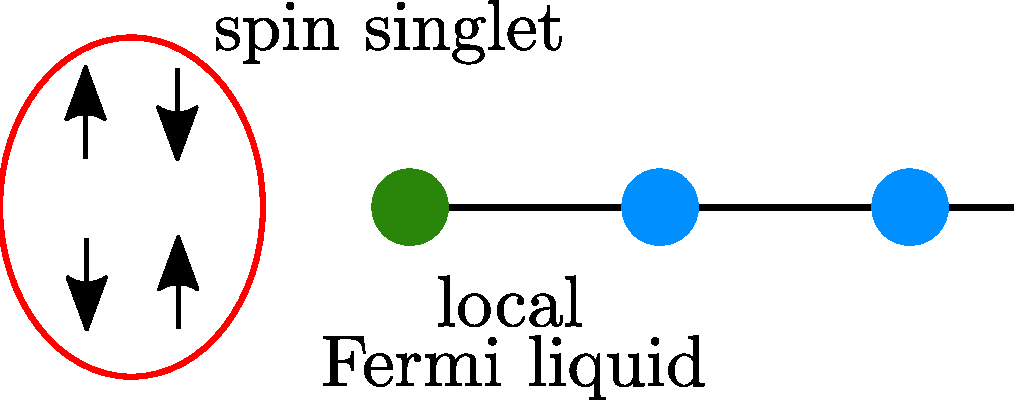
\includegraphics[width=\textwidth]{figures/cloud_lFL.pdf}}
	\only<4-5>{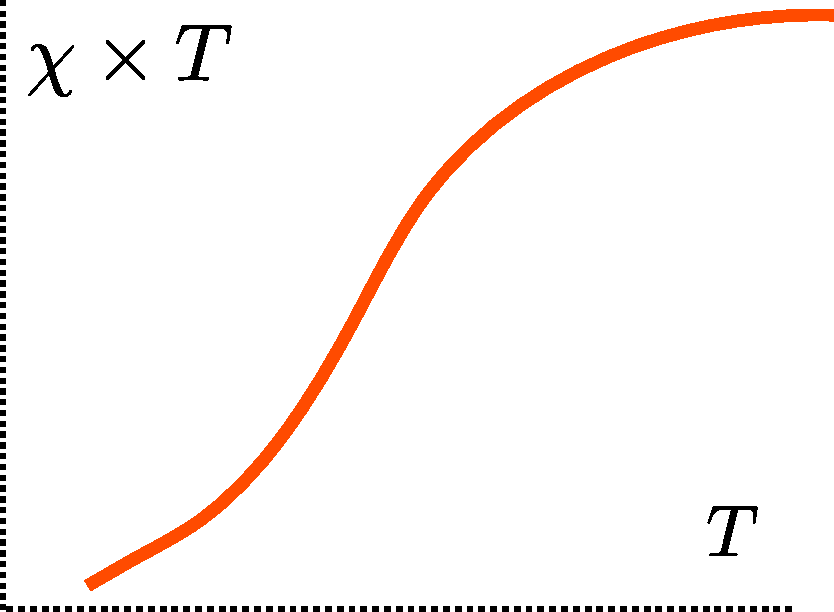
\includegraphics[width=\textwidth]{figures/chi_schematic.pdf}}
\end{minipage}
\begin{textblock*}{\textwidth}(40pt, 0.8\textheight)
	\centering
	\hspace*{\fill}
	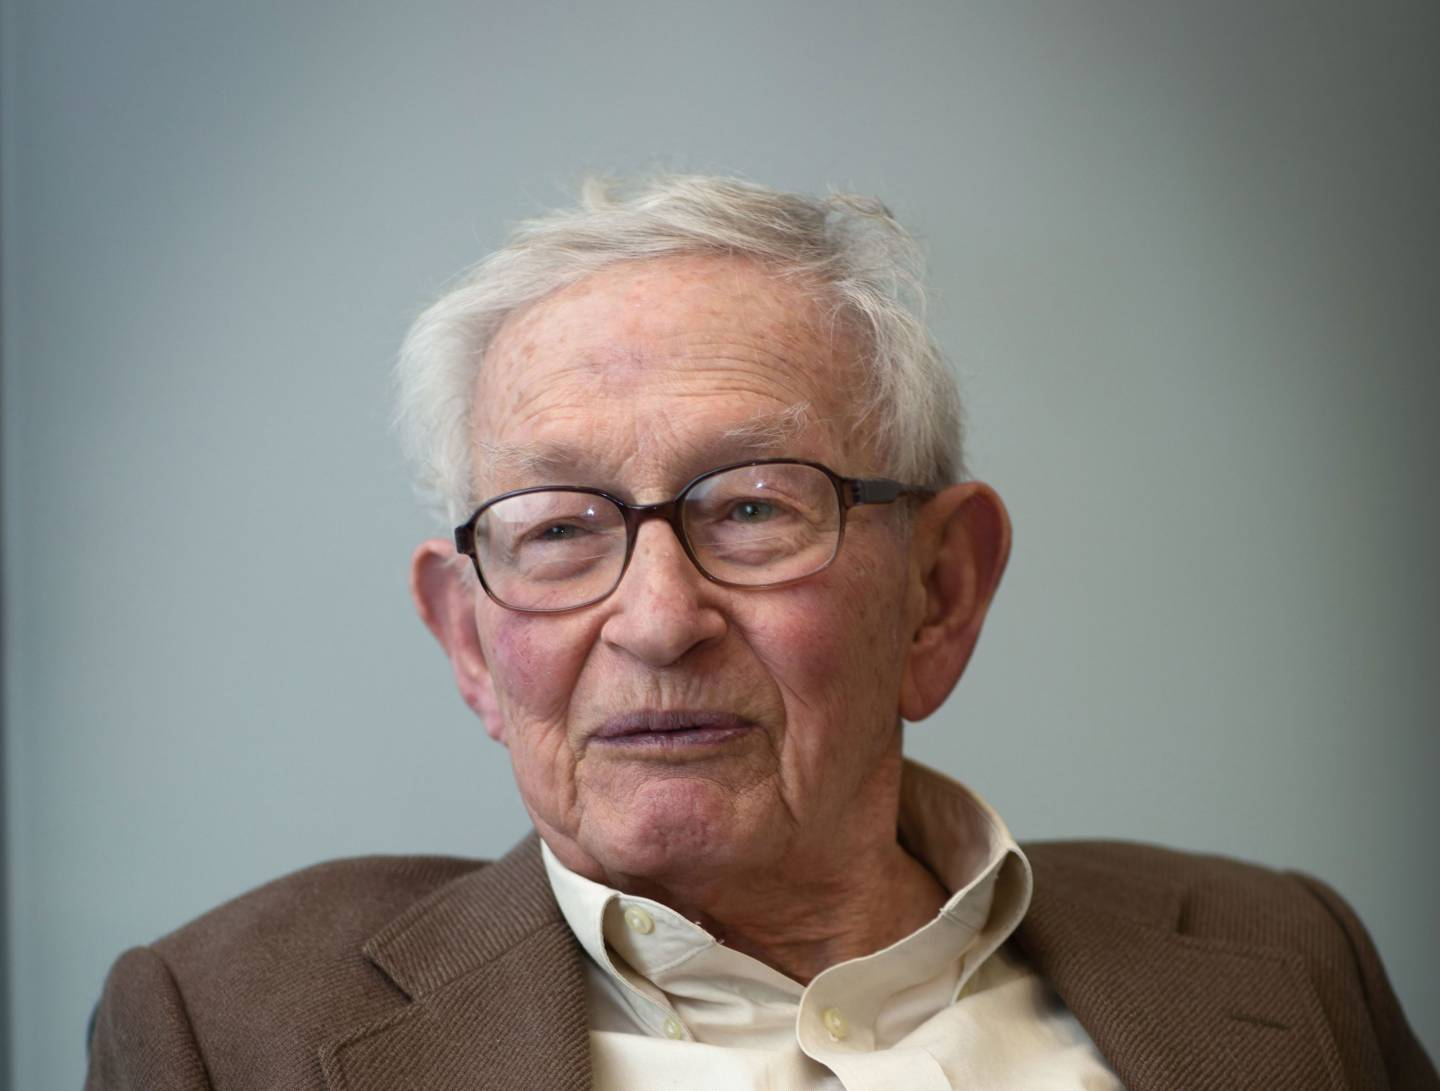
\includegraphics[height=30pt]{figures/pwanderson.jpg}
	\hspace*{\fill}
	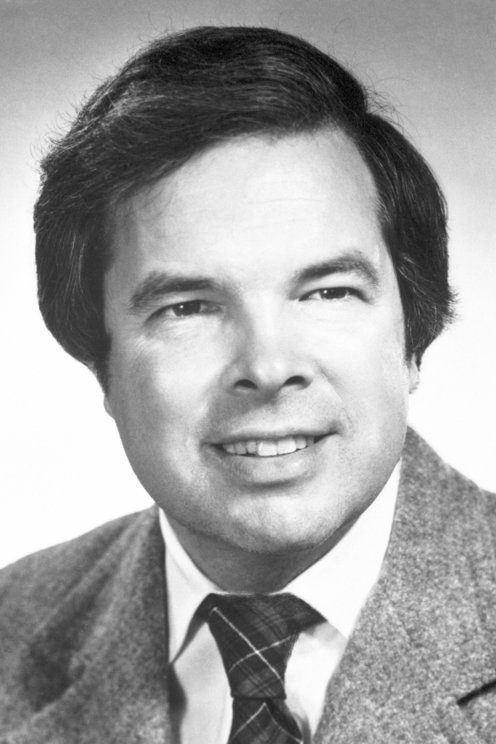
\includegraphics[height=30pt]{figures/kgwilson.jpg}
	\hspace*{\fill}
	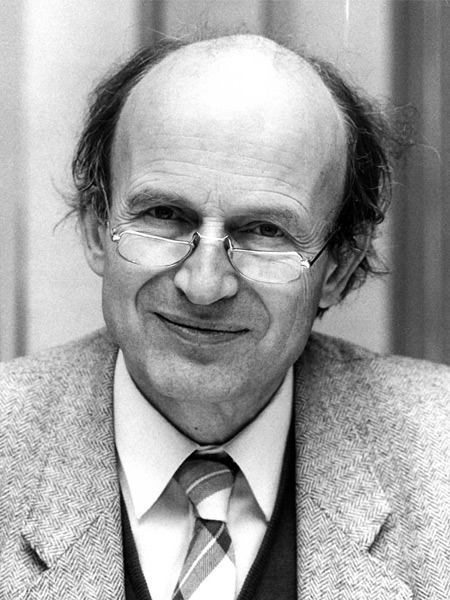
\includegraphics[height=30pt]{figures/nozieres.jpg}
	\hspace*{\fill}
\end{textblock*}
\footcite{anderson1969exact,anderson1970,wilson1975,andreiKondoreview,andrei_kondo,wiegmann_kondoexact_1981,nozieres1974fermi}
}
\end{frame}

\section{What's left to understand?}
\begin{frame}[noframenumbering]{What's Left To Understand?}
  
\begin{itemize}[<+-|alert@+>]
	\item Finite \(J\) effective Hamiltonian at fixed point
	\vspace*{20pt}
	\item Hamiltonian for the itinerant electrons forming the \focus{macroscopic singlet}
	\vspace*{20pt}
	\item Nature of correlations inside the Kondo cloud: \focus{Fermi liquid vs off-diagonal} - what leads to the maximally entangled singlet?
	\vspace*{20pt}
	\item Behaviour of \focus{many-particle entanglement} and many-body correlation under RG flow
\end{itemize}

\end{frame}

\section{The Unitary Renormalization Group Method}
\begin{frame}[noframenumbering]{The Unitary Renormalization Group Method}
\footcite{anirbanurg1,anirbanurg2}

\only<1-3>{
\head{The General Idea}
\begin{minipage}{0.8\textwidth}
\begin{itemize}[<+-|alert@+>]
	\item Apply unitary many-body transformations to the Hamiltonian\\[10pt]
	\item Successively decouple high energy states\\[10pt]
	\item Obtain sequence of Hamiltonians and hence scaling equations
\end{itemize}
\end{minipage}
\begin{minipage}{0.15\textwidth}
\begin{figure}
	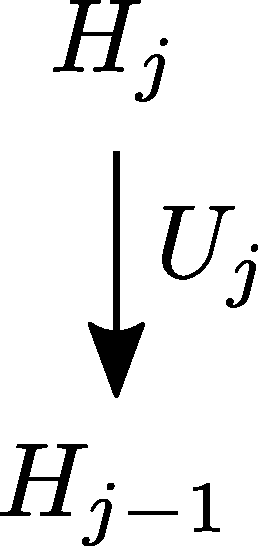
\includegraphics[width=0.7\textwidth]{figures/urg_schematic.pdf}
\end{figure}
\end{minipage}
}

\only<4>{
\head{Select a UV-IR Scheme}
\vspace*{\fill}

\begin{minipage}{0.5\textwidth}
\centering
\focus{UV shell}
\begin{gather*}
	\vec k_N ~~ \left(\text{zeroth RG step}\right)\\
\vdots\\ 
\vec k_j ~ ~ \left(j^\text{th} \text{ RG step}\right) \\
\vdots\\
\vec k_1 ~ ~ \left(\text{Fermi surface}\right)
\end{gather*}
\focus{IR shell}
\end{minipage}
\hspace*{\fill}
\begin{minipage}{0.4\textwidth}
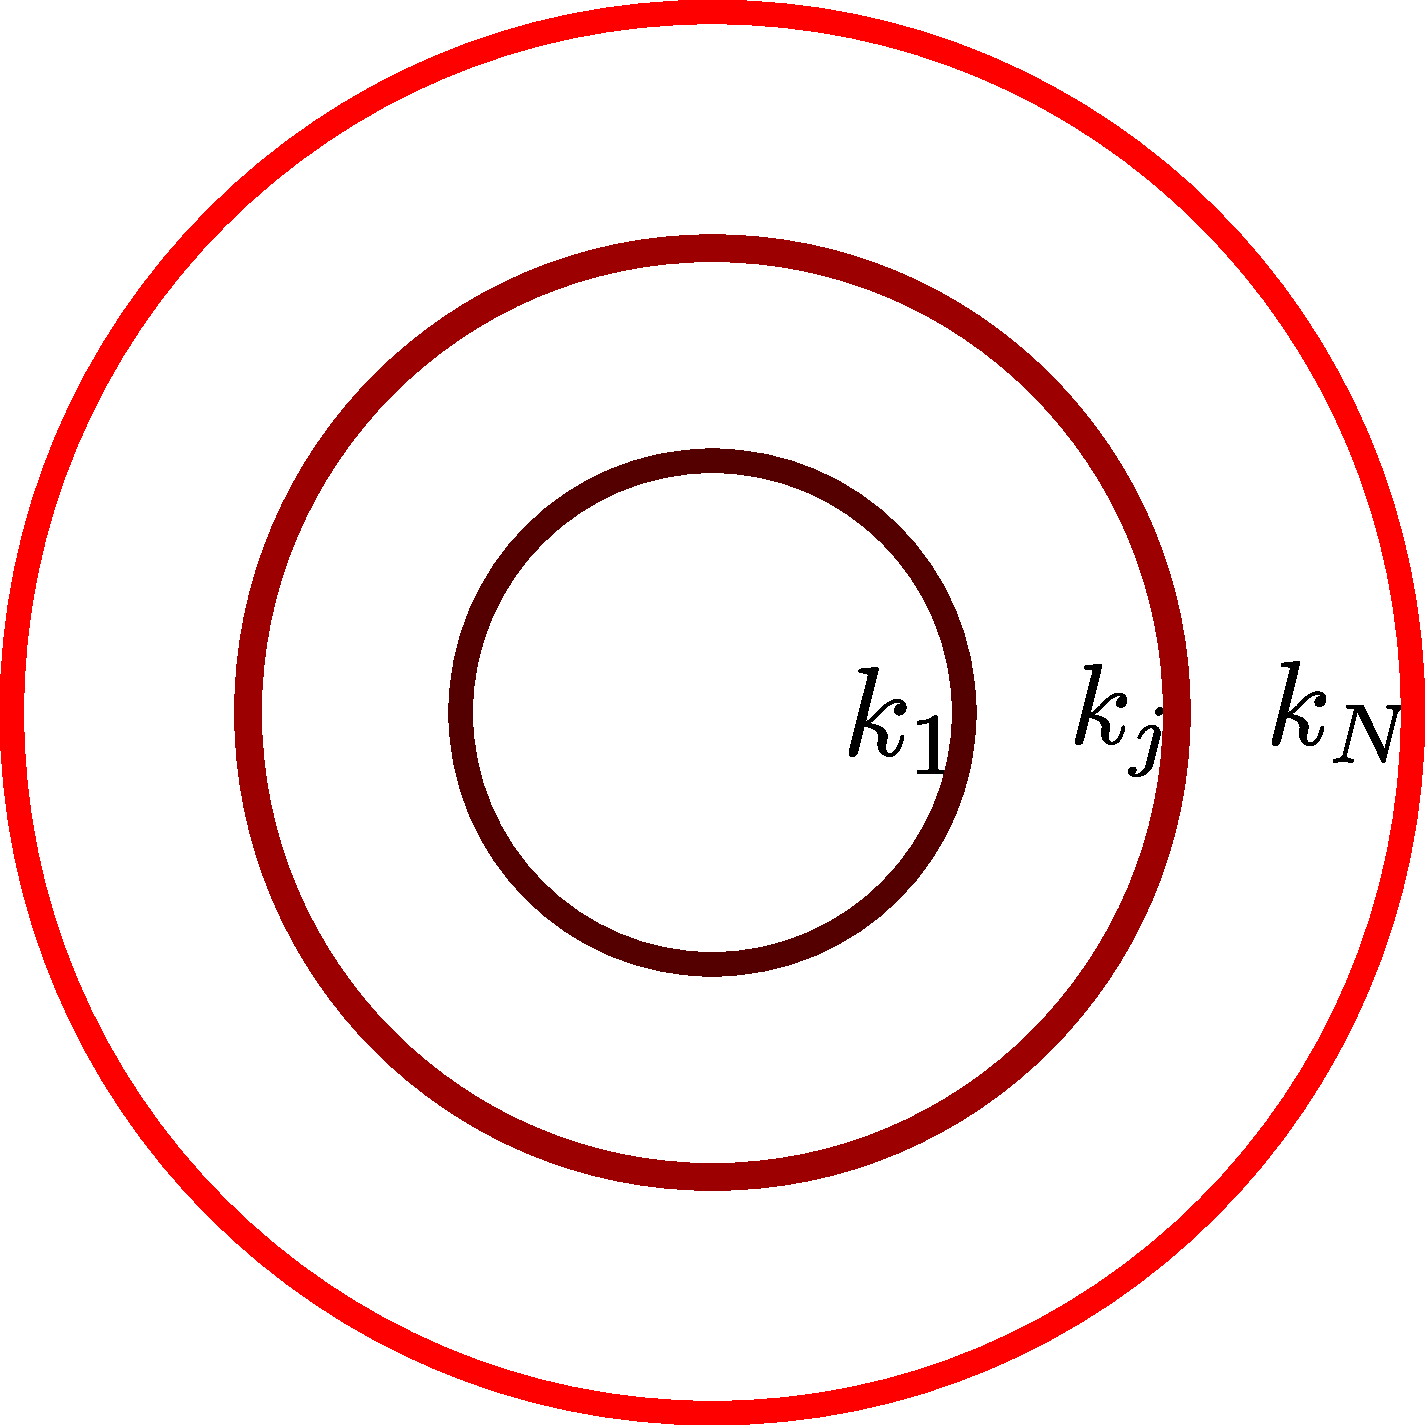
\includegraphics[width=0.9\textwidth]{figures/uv_ir_scheme.pdf}
\end{minipage}
\vspace*{\fill}
}

\only<5>{
\vspace*{-20pt}
\head{Write Hamiltonian in the basis of \(\vec k_j\)}
\vspace*{\fill}

\begin{minipage}{0.4\textwidth}
	\vspace*{-30pt}
	\[H_{(j)} = H_1 \hat n_j + H_0 \left(1 - \hat n_j\right) + c^\dagger_j T + T^\dagger c_j\]
\[
 {2^{j-1} \text{-dim.}} \longrightarrow \begin{cases}
	H_1, H_0 \longrightarrow \text{diagonal parts}\\
T \longrightarrow \text{off-diagonal part}
\end{cases}
\]
\end{minipage}
\hspace*{\fill}
\begin{minipage}{0.5\textwidth}
\begin{figure}
	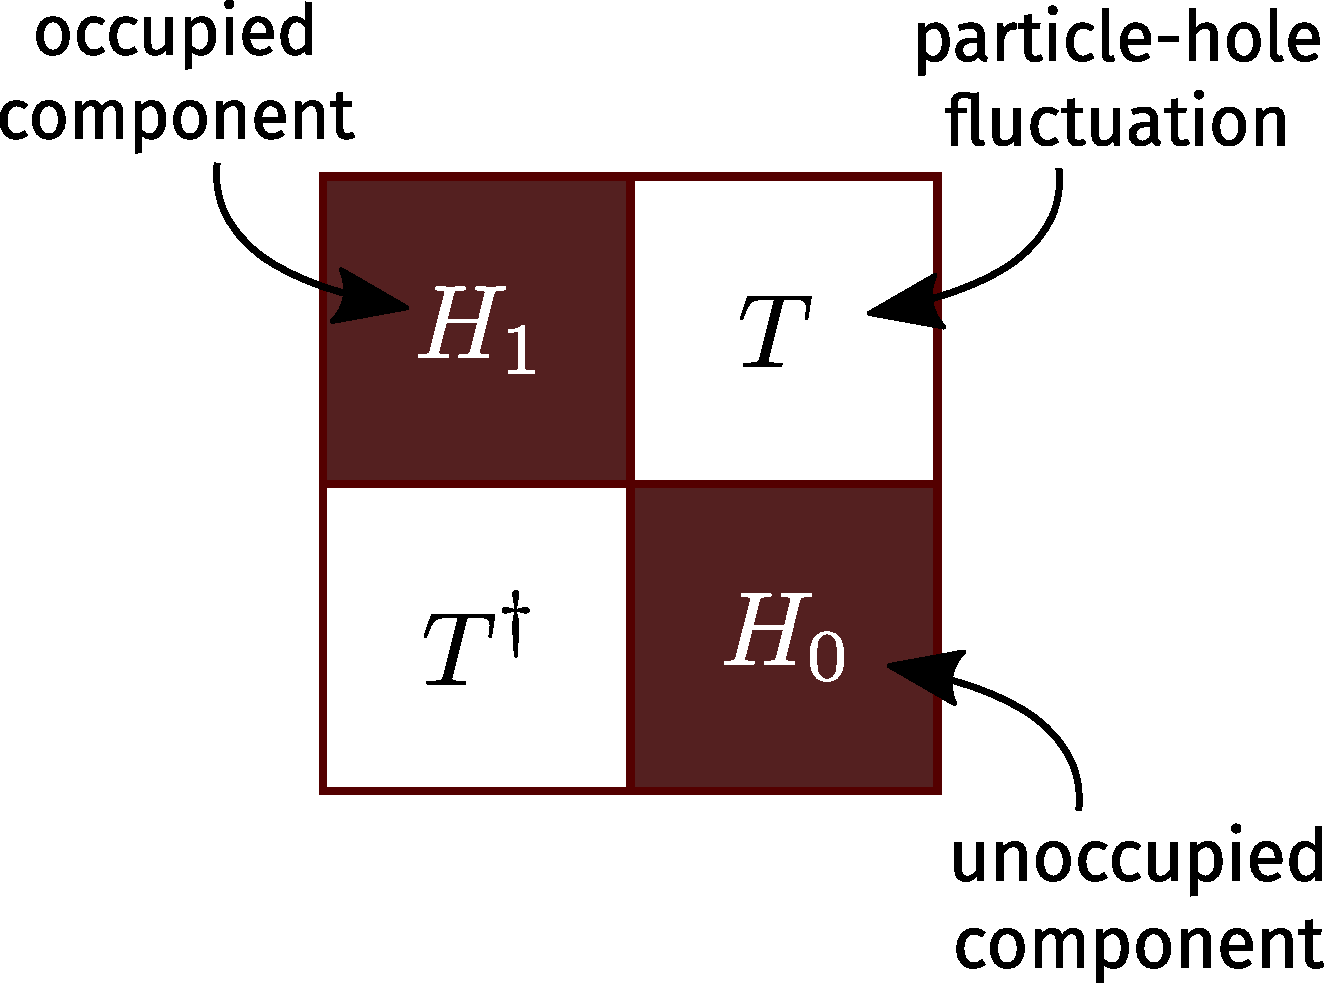
\includegraphics[width=0.9\textwidth]{figures/urg_ham.pdf}
\end{figure}
\end{minipage}
}
\only<6>{
\vspace*{-10pt}
\head{Rotate Hamiltonian and kill off-diagonal blocks}

\vspace*{\fill}

\begin{minipage}{0.45\textwidth}
	\[H_{(j-1)} = U_{(j)} H_{(j)} U_{(j)}^\dagger\]
	\[U_{(j)} = \frac{1}{\sqrt 2}\left(1 - \eta_{(j)} + \eta_{(j)}^\dagger\right) \]
	\[ \eta^\dagger_{(j)} = \frac{1}{\hat \omega_{(j)} - H_D}c^\dagger_j T \Bigg \} \rightarrow {\text{many-particle}\atop{\text{rotation}}}\]
\[ \left\{\eta_{(j)}, \eta^\dagger_{(j)}\right\} = 1\]
\vspace*{\fill}
\end{minipage}
\hspace*{\fill}
\begin{minipage}{0.5\textwidth}
\begin{figure}
	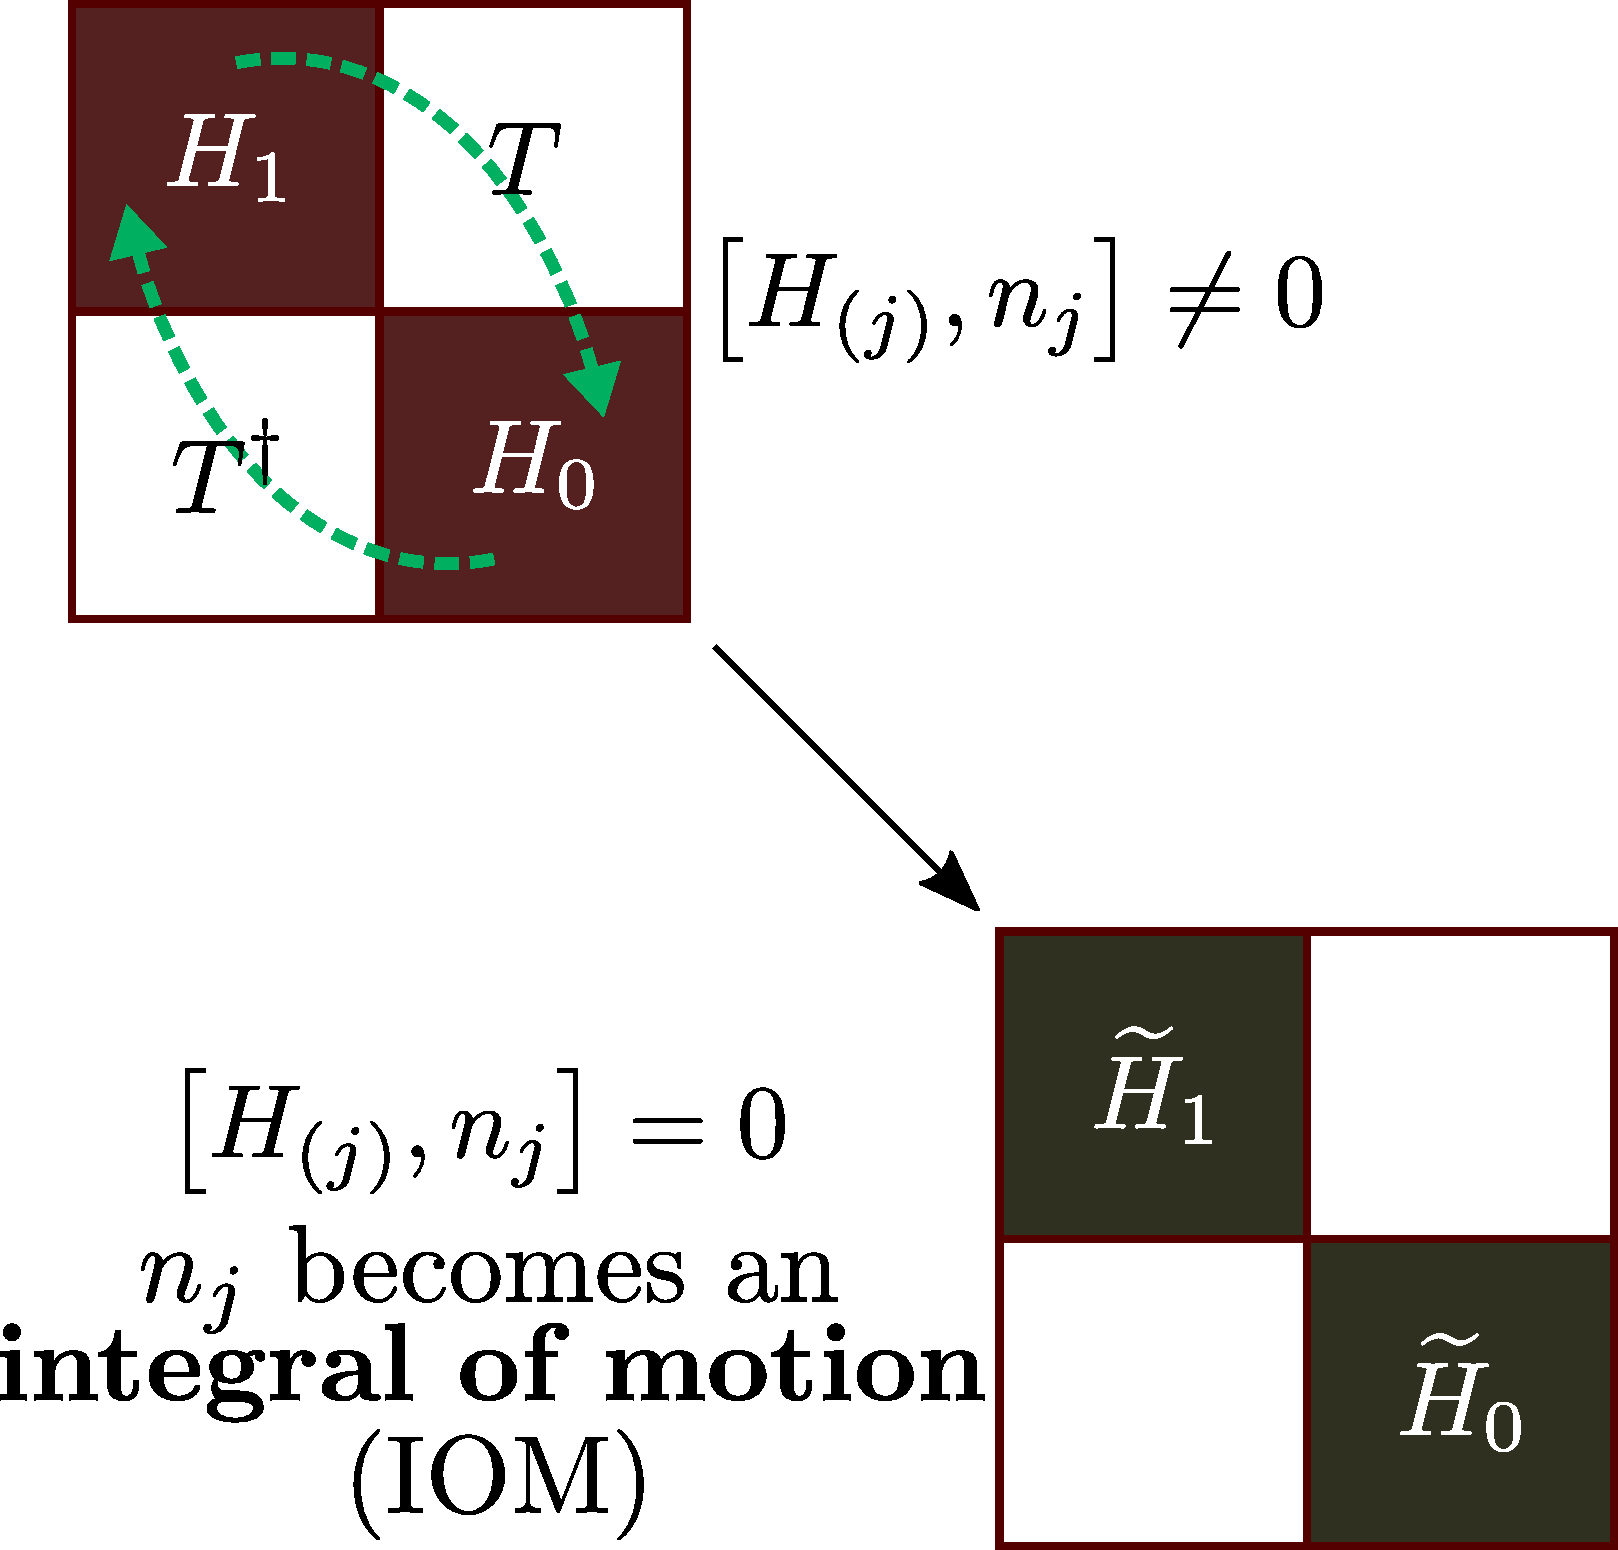
\includegraphics[width=0.8\textwidth]{figures/urg_rot.pdf}
\end{figure}
\end{minipage}
}

\only<7>{

\head{Repeat with renormalised Hamiltonian}

\begin{minipage}{0.53\textwidth}
	\[H_{(j-1)} = \widetilde H_1 \hat n_j + \widetilde H_0 \left(1 - \hat n_j\right)\]
	\[\widetilde H_1 = H_1 \hat n_{j-1} + H_0 \left(1 - \hat n_{j-1}\right) + c^\dagger_{j-1} T + T^\dagger c_{j-1}\]
\vspace*{\fill}
\end{minipage}
\hspace*{\fill}
\begin{minipage}{0.45\textwidth}
\begin{figure}
	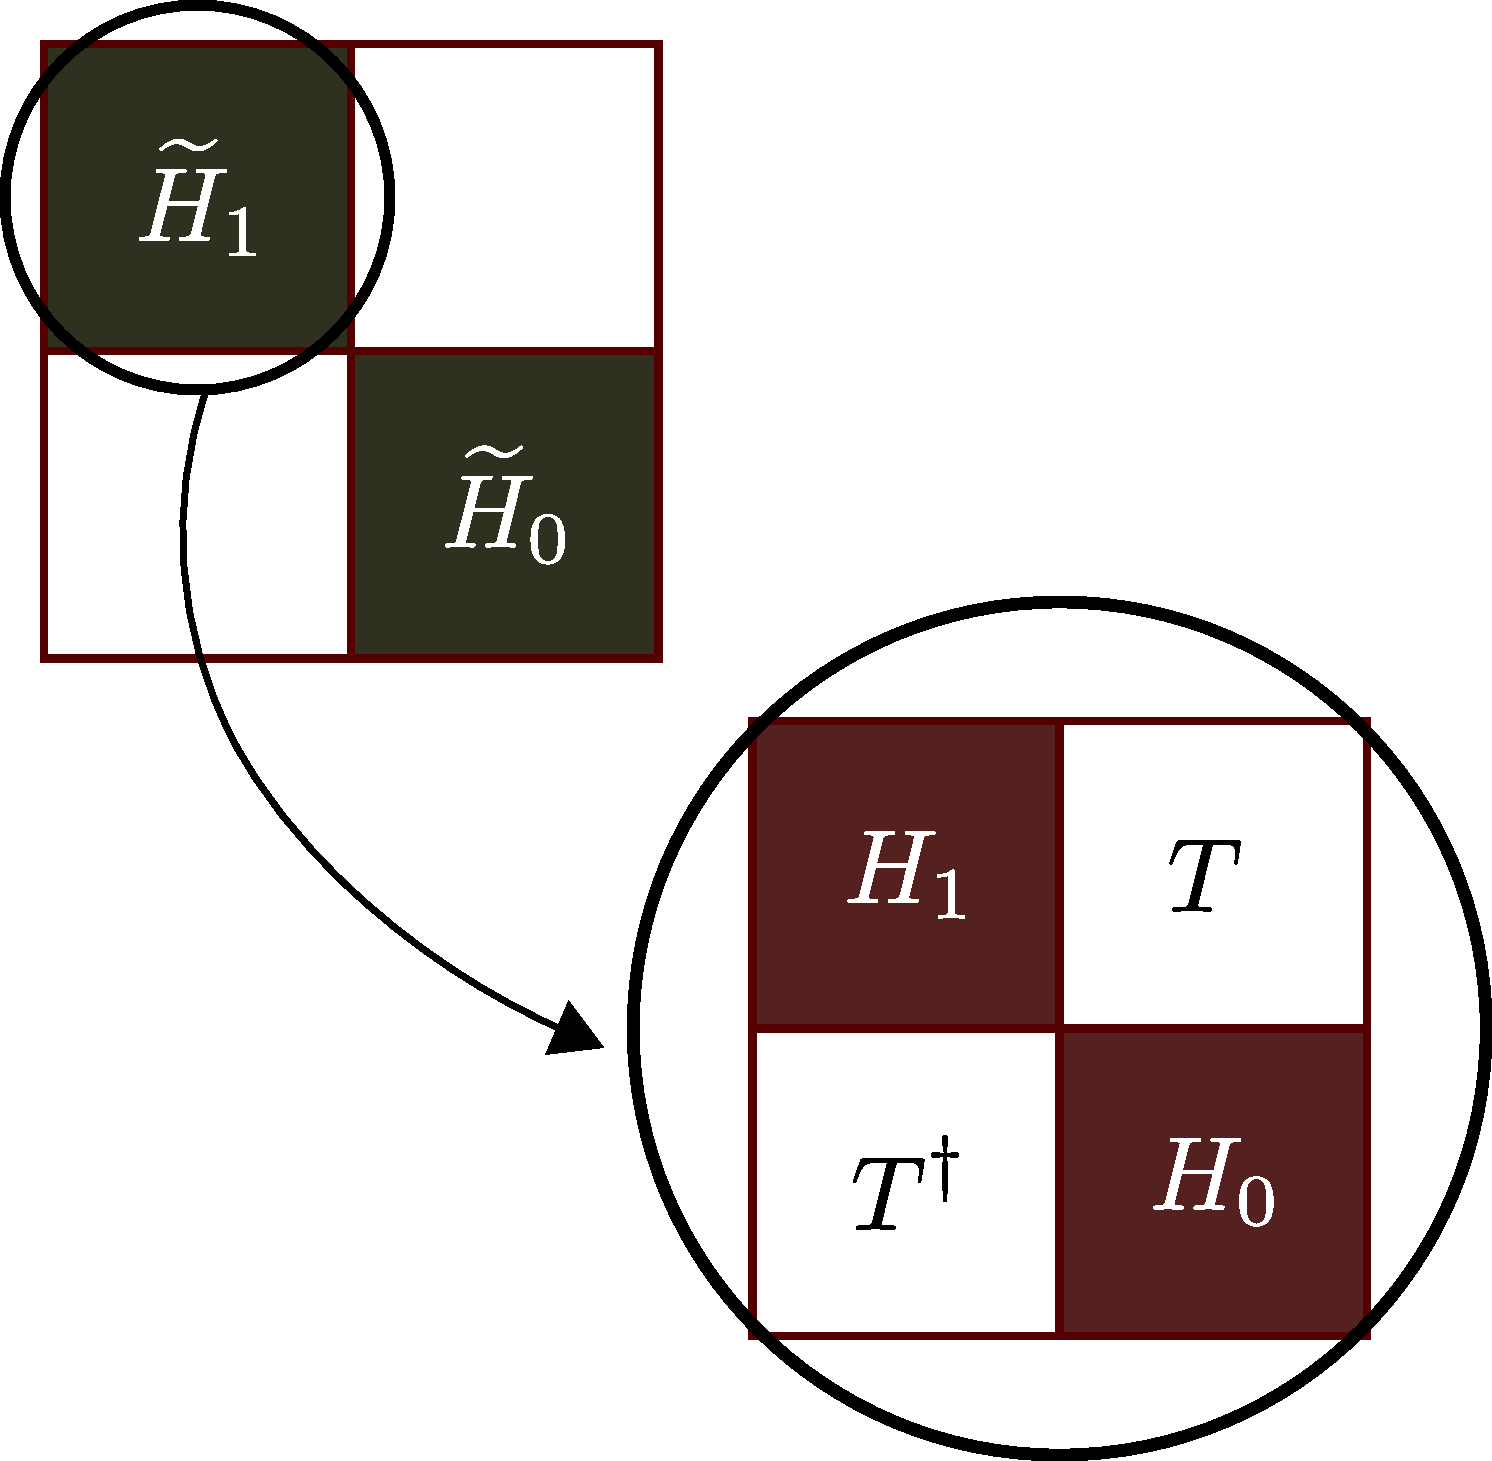
\includegraphics[width=\textwidth]{figures/urg_next.pdf}
\end{figure}
\end{minipage}
}

\only<8>{
\vspace*{-30pt}
\head{RG Equations and Denominator Fixed Point}

\vspace*{40pt}
\begin{minipage}{0.4\textwidth}
	\centering
\[ \Delta H_{(j)} = \left(\hat n_j - \frac{1}{2}\right) \left\{c^\dagger_j T, \eta_{(j)}\right\} \]

\[\eta^\dagger_{(j)} = \frac{1}{\hat \omega_{(j)} - H_D}c^\dagger_j T\] 

\[\text{\focus{Fixed point:}}~ ~ ~\hat \omega_{(j^*)} - \left(H_D\right)^* = 0\]
\end{minipage}
\hspace*{\fill}
\begin{minipage}{0.58\textwidth}
	\centering
	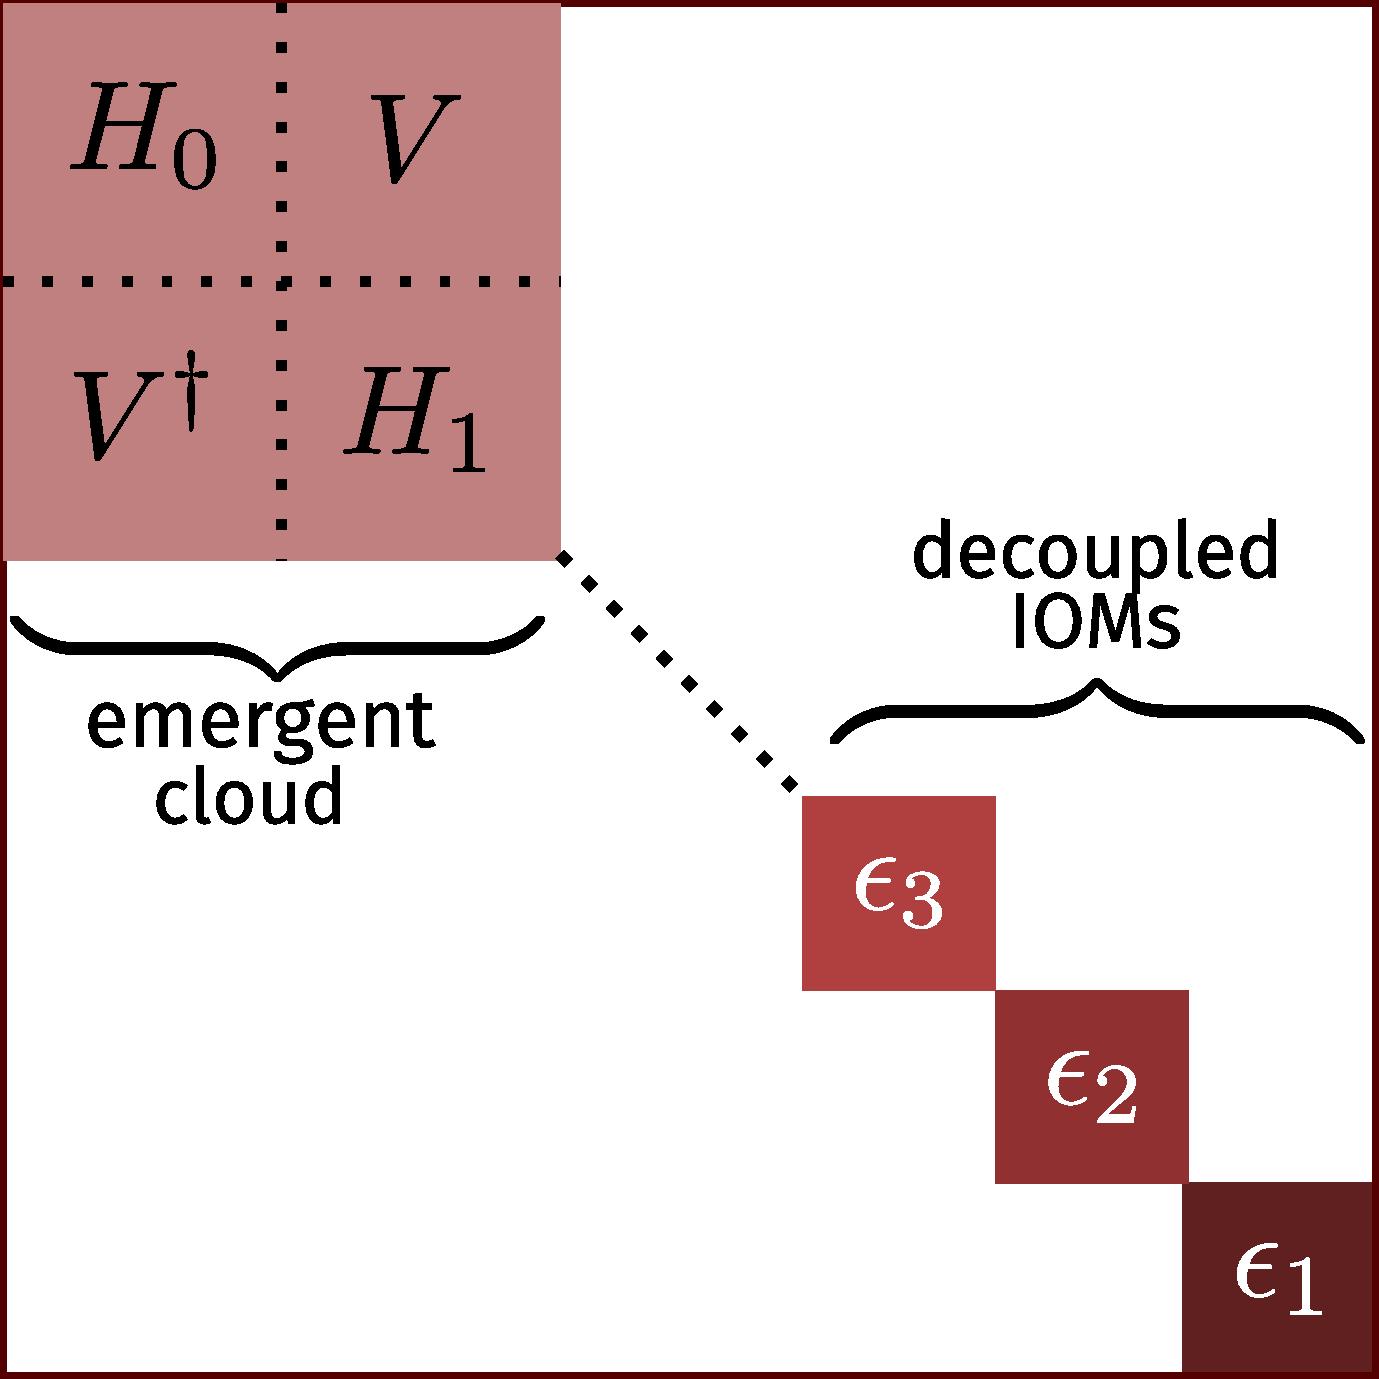
\includegraphics[width=0.65\textwidth]{figures/urg_ham_full.pdf}
\end{minipage}
\vspace*{\fill}
}
\end{frame}

\begin{frame}[noframenumbering]{The Unitary Renormalization Group Method}
\head{Novel Features of the Method}
% \hspace*{-20pt}
\begin{minipage}{0.65\textwidth}
\begin{itemize}[<+-|alert@+>]
	\item \focus{Quantum fluctuation scale} \(\hat \omega\)	that tracks all orders of renormalisation\\[10pt]
	\item Finite-valued fixed points for finite systems - leads to \focus{emergent degrees of freedom}\\[10pt]
	\item \focus{Spectrum-preserving} unitary transformations - partition function does not change\\[10pt]
	\item Tractable low-energy effective Hamiltonians - allows \focus{renormalised perturbation theory} around them 
\end{itemize}
\end{minipage}
\hspace*{\fill}
\begin{minipage}{0.3\textwidth}
\begin{flushleft}
	\(H_{(j-1)} = U_{(j)} H_{(j)} U_{(j)}^\dagger\)\\[15pt]
	\(U_{(j)} = \frac{1}{\sqrt 2}\left(1 - \eta_{(j)} + \eta_{(j)}^\dagger\right) \)\\[15pt]
	\( \eta^\dagger_{(j)} = \frac{1}{\hat \omega_{(j)} - H_D}c^\dagger_j T\)\\[15pt]
	\( \Delta H_{(j)} = \left(\hat n_j - \frac{1}{2}\right) \left\{c^\dagger_j T, \eta_{(j)}\right\} \)
\end{flushleft}
\end{minipage}
\end{frame}

\section{URG of the Kondo Model}
\begin{frame}[noframenumbering]{URG of the Kondo Model}
	\only<1>{\head{RG Equation}}
	\only<2>{\head{RG flows and fixed points}}
	\only<3>{\head{Phase diagram}}
	\only<4>{\head{Kondo cloud length \(\xi_K\)}}
	\only<5>{\head{Fixed point Hamiltonian}}
	\only<6>{\head{Approach towards the continuum}}

\centering

\begin{minipage}{0.35\textwidth}
{
	\[\Delta J_{(j)} = \frac{n_j ~ J_{(j)}^2 ~ \left(\omega_{(j)} - \frac{D_j}{2}\right)}{\left(\omega_{(j)} - \frac{D_j}{2}\right)^2 - \frac{1}{16}J_{(j)}^2}\]
	\[ J^* = 4\left(\omega^* - \frac{1}{2}D^*\right)\]
	\[D^* \longrightarrow \text{ emergent window}\]
	\only<2->{\[\omega_{(j)} > \frac{D_j}{2}\]}
}
\end{minipage}
\hspace*{\fill}
\begin{minipage}{0.6\textwidth}
\centering
\only<+>{

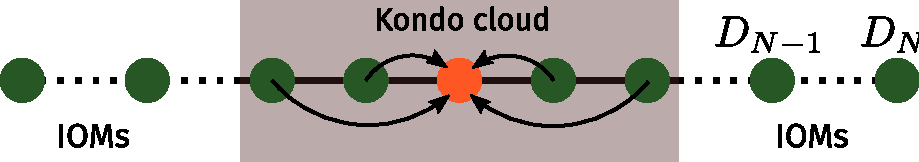
\includegraphics[width=\textwidth]{figures/kondo_fp_1D.pdf}
\\[10pt]

\focus{For \(J_{(j)} \ll D_j\), we recover weak-coupling form}: 
\[\frac{\Delta J_{(j)}}{\Delta \ln D_j} \sim n_j ~ J_{(j)}^2\]
}
\only<+>{
\[K_{(j)} = J_{(j)}\left(\omega^* - \frac{1}{2}D^*\right)^{-1}, ~ ~ K^* = 4\]
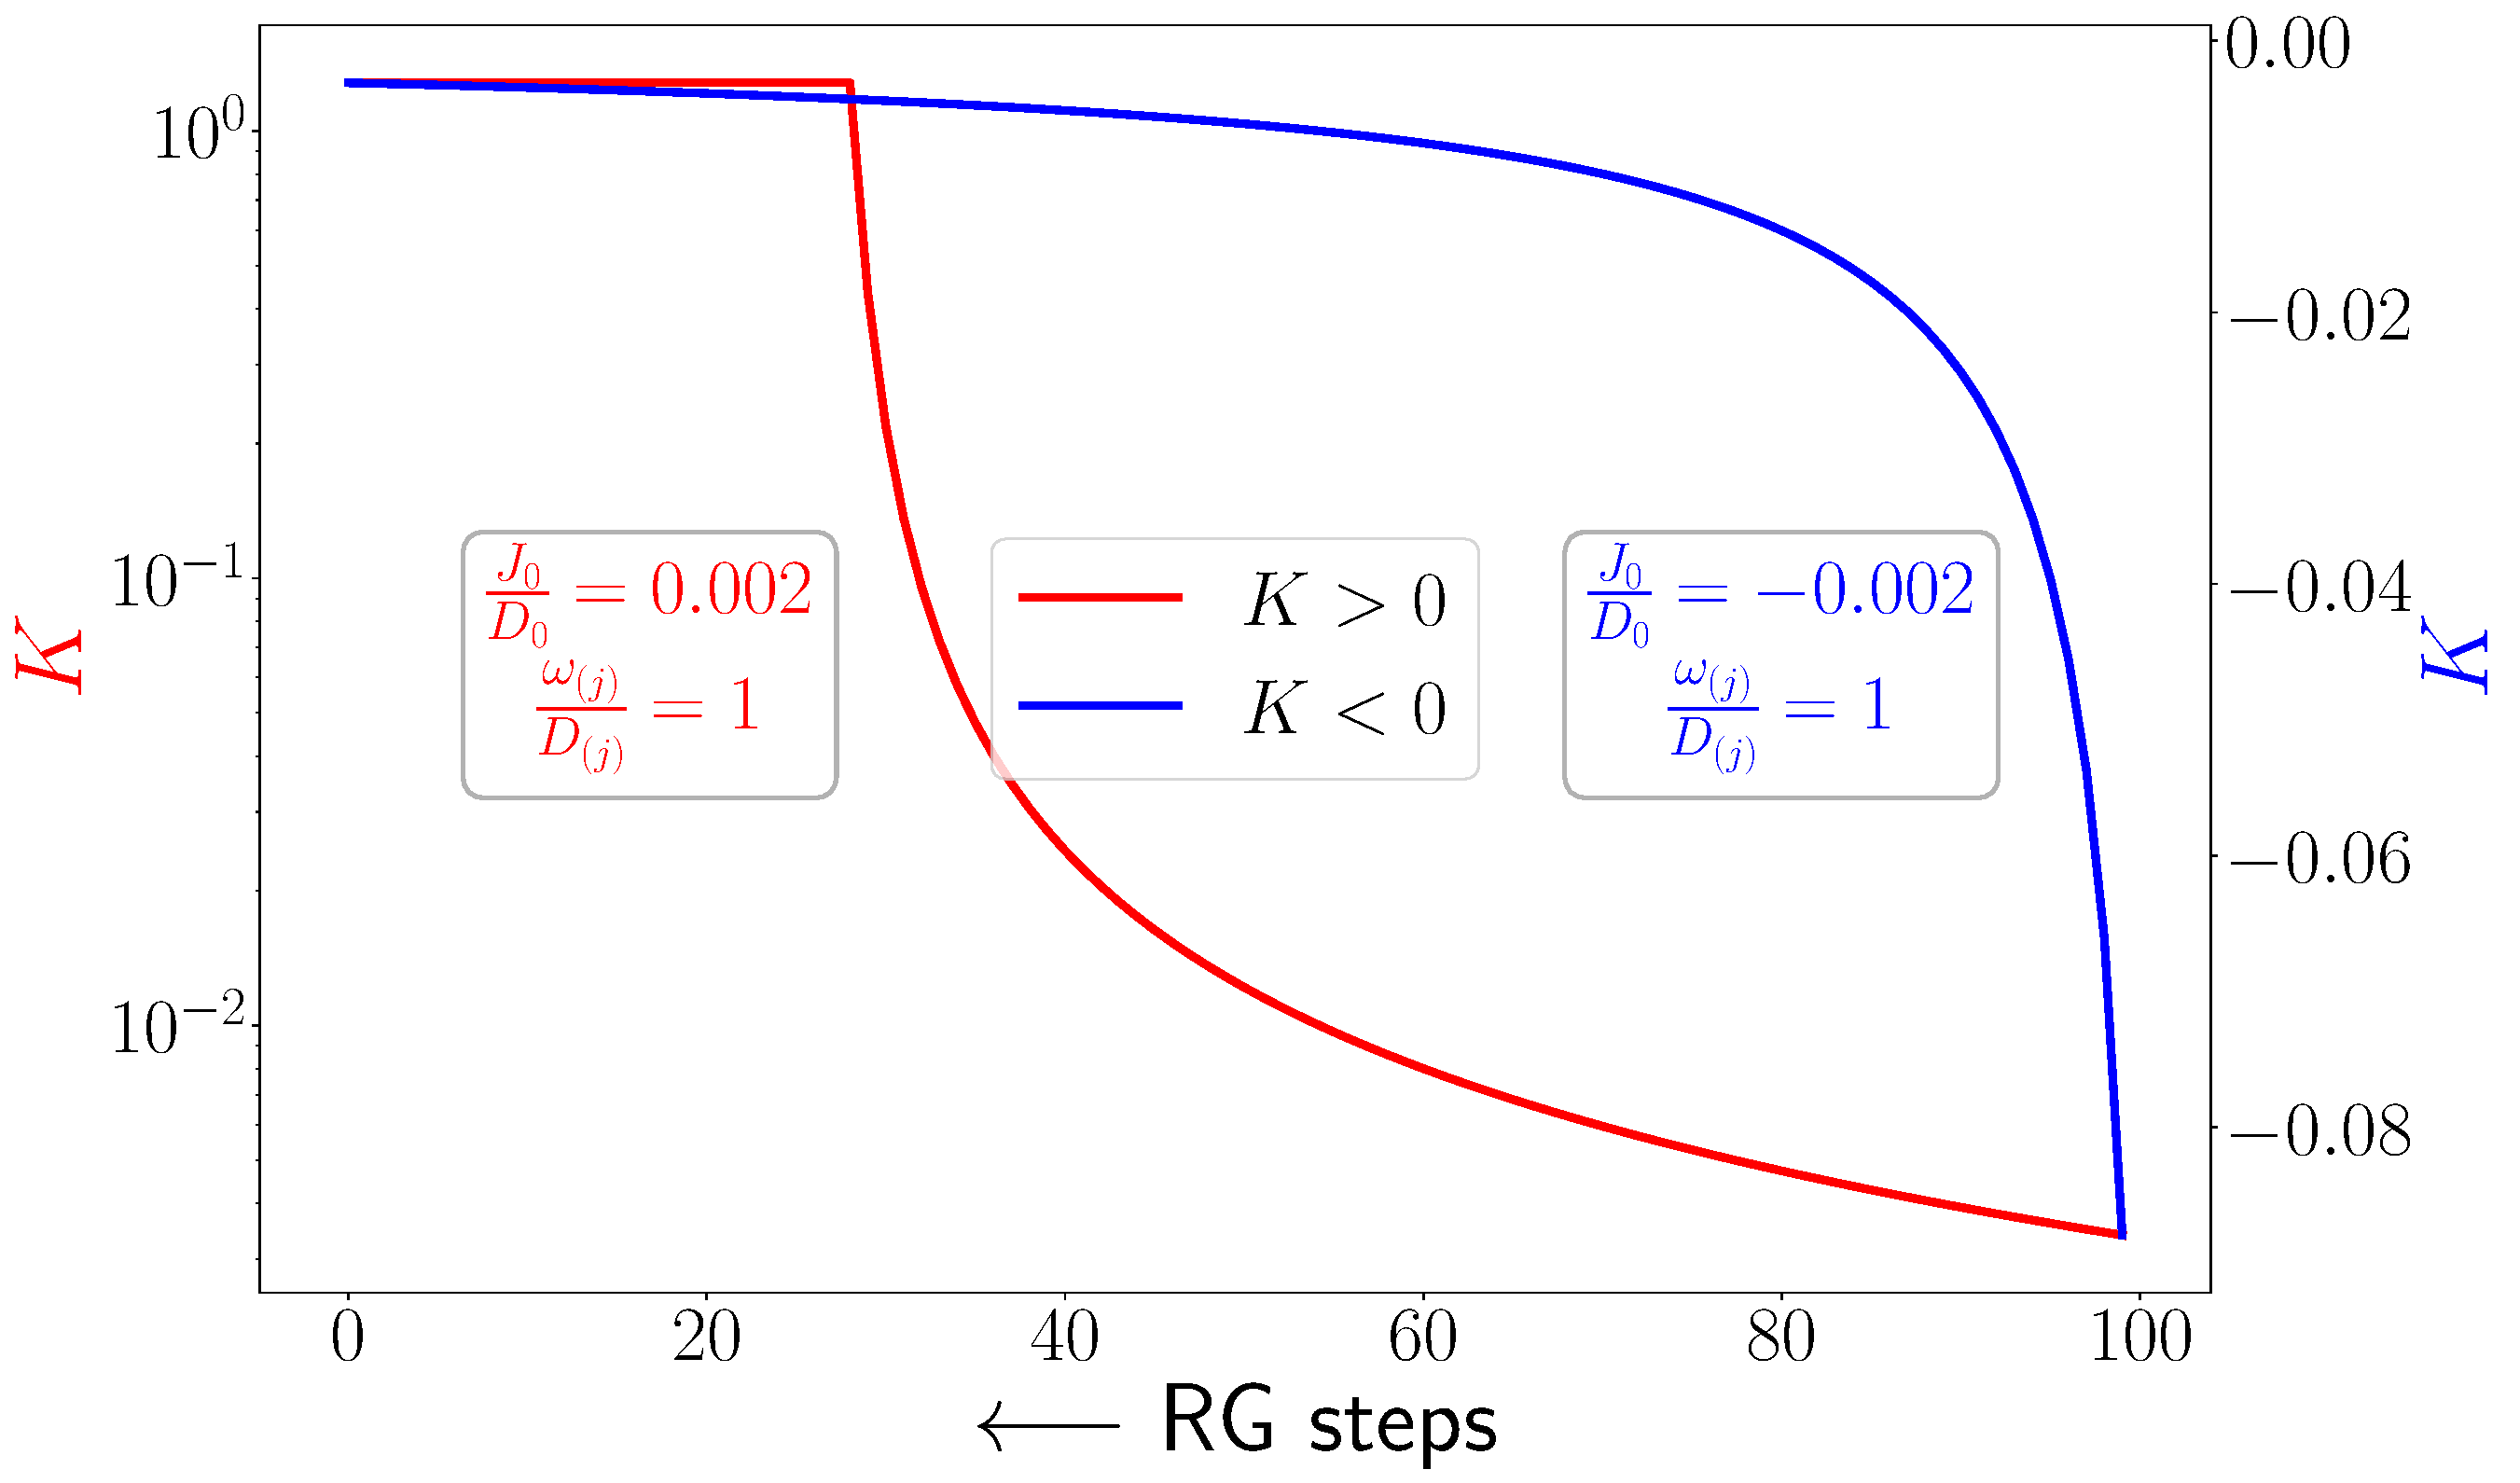
\includegraphics[width=\textwidth]{figures/RG_flow.pdf}
}
\only<+>{
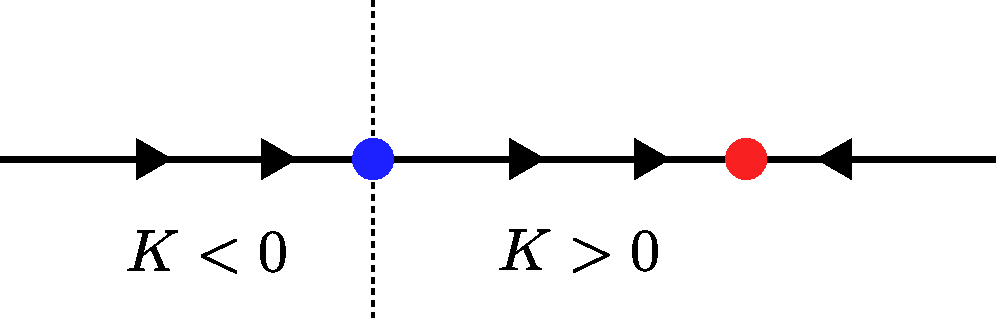
\includegraphics[width=0.9\textwidth]{figures/kondo_phase.pdf}

\begin{itemize}
\item {Decay towards FM fixed point for \(J<0\)}\\[10pt]
\item {Attractive flow towards AFM fixed point for \(J>0\)}
\end{itemize}
}
\only<+>{
	\centering
	% \[ \xi_K = \frac{2\pi}{\Lambda^*} = \frac{2\pi}{\Lambda_{0}}\exp\left(-\frac{1}{2n(0)}+\frac{1}{n(0)K_{0}}+\frac{K_{0}}{n(0)16}\right)\]
	\[\hspace*{-10pt} T_K = \frac{\hbar v_{F}\Lambda_{0}}{k_{B}}\exp\left(\frac{1}{2n(0)}-\frac{1}{n(0)K_{0}}-\frac{K_{0}}{n(0)16}\right), ~ ~ \xi_K = \frac{h v_F}{k_B T_K}\]
	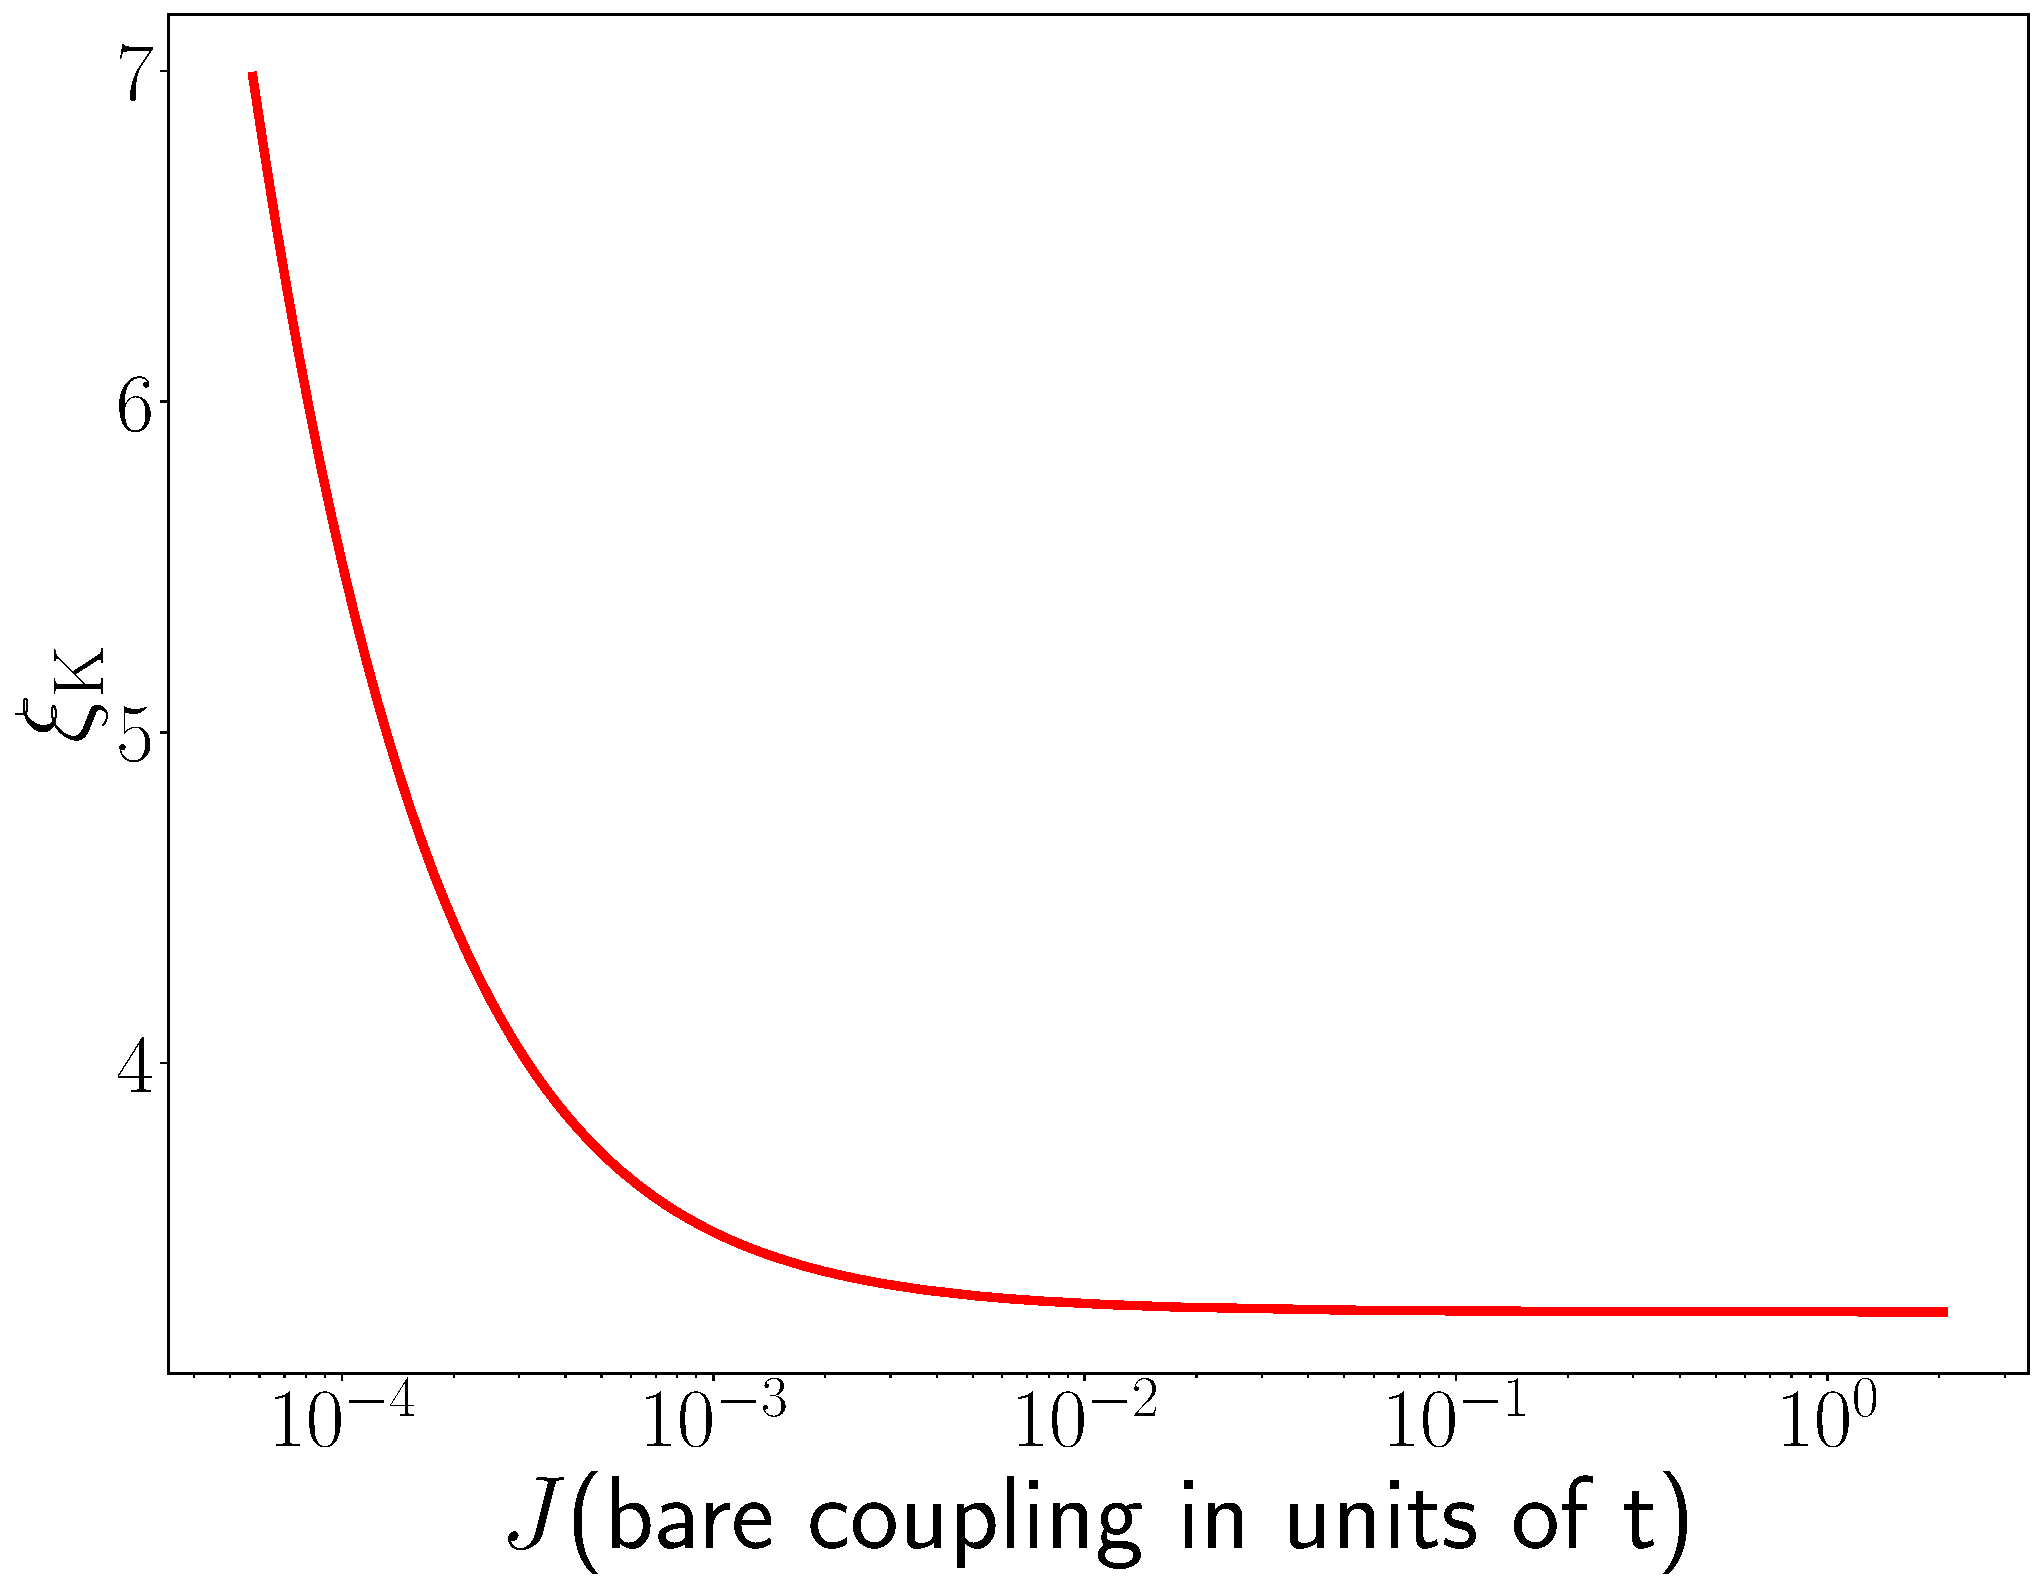
\includegraphics[width=0.8\textwidth]{figures/xi_k.pdf}
}
\only<+>{
	\[H^* = \underbrace{\sum_{k < k^*,\sigma}\epsilon_{k}\hat{n}_{k\sigma} ~ + ~ J^* \vec{S}_d\cdot \vec{s}_<}_\text{emergent window} ~ + ~\underbrace{\sum_{j=j^*}^N J^{j}S_d^{z}\sum_{|q| = q_j}s^{z}_{q_j}}_\text{integrals of motion}\]
	\[\vec{s}_< = \frac{1}{2}\sum_{k,k^\prime < k^*}c^{\dagger}_{k\alpha}\vec{\sigma}_{\alpha\beta}c_{k^\prime,\beta}\]
	\[s^z_{q} = \frac{1}{2}\left(\hat n_{q \uparrow} - \hat n_{q \downarrow}\right)\]
}
\only<+>{
\[J^* \to \infty \text{ in thermodynamic limit}\]
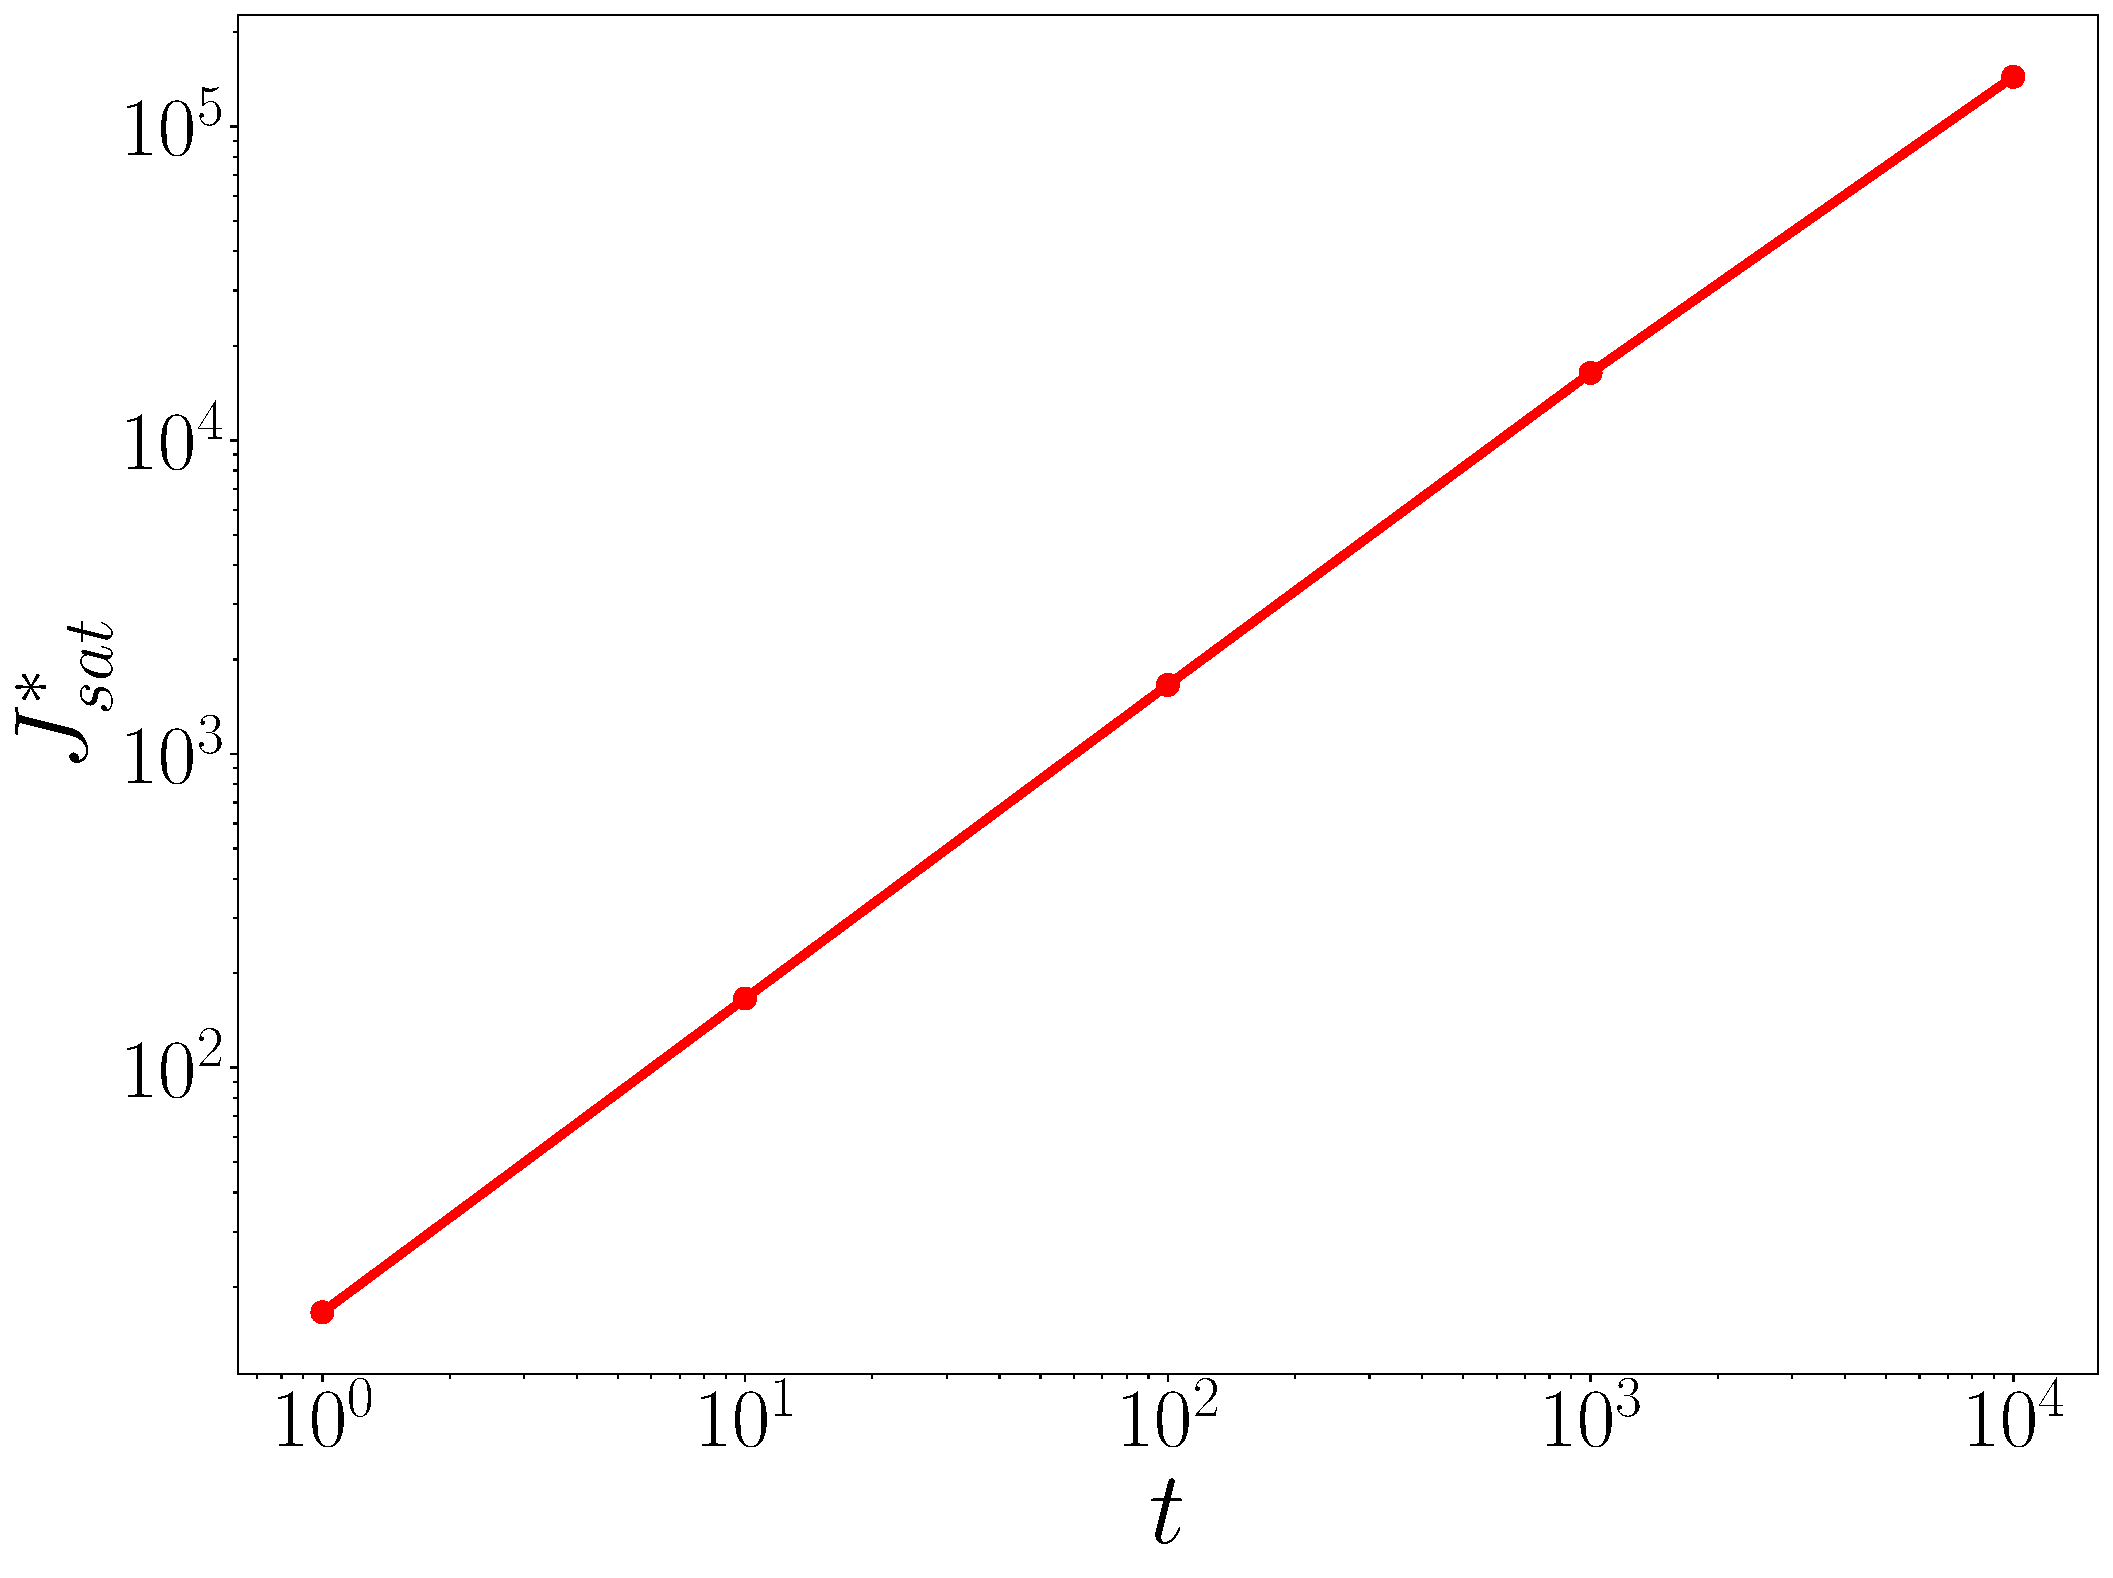
\includegraphics[width=0.8\textwidth]{figures/KondoCouplingVst.pdf}
}
\end{minipage}

\only<1>{\footcite{anderson1970,sorensen_erik_affleck_1996}}
\only<5>{\footcite{wilson1975}}

\end{frame}


\section{Zero-bandwidth limit of fixed point Hamiltonian}
\begin{frame}[noframenumbering]{Zero-bandwidth limit of fixed point Hamiltonian}
\only<1>{
	\head{Route to the zero-bandwidth model}
	At strong-coupling fixed point,
	\begin{itemize}
	\item kinetic energy acts as a perturbation
	\item \focus{compress the bandwidth to just the Fermi surface}

	\[H^*_\text{zero bw} = J \vec{S}_d\cdot\vec{s}_< + \left(\epsilon_F - \mu\right) \hat n_{k_F}~ ~ \left(\text{center of motion}\right)\]\\[10pt]

	\item Setting \(\mu = \epsilon_F\) gives a \focus{two-spin Heisenberg model}

	\[H^*_\text{zero} = J^* \vec{S}_d\cdot\vec{s}_<\]
	\end{itemize}
}
\only<2>{
	\head{Effective two-site problem}
	\centering

	\[H^*_\text{zero} = J^* \vec{S}_d\cdot\vec{s}_< + H^*_\text{IOMS}\]

	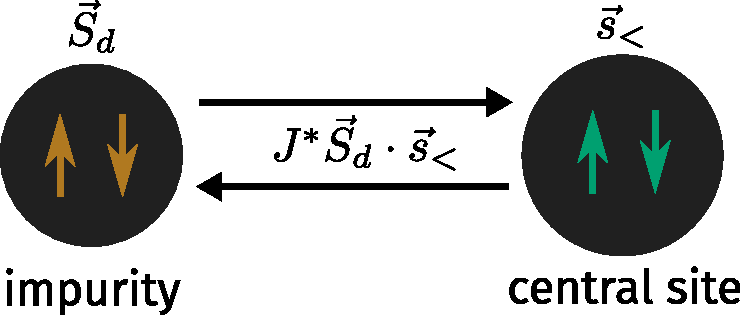
\includegraphics[width=0.4\textwidth]{figures/kondo_zeromode.pdf}

	\[\text{Singlet ground state: }~ ~\ket{\Psi}_\text{gs} = \frac{1}{\sqrt 2}\left(\ket{\uparrow,\downarrow} - \ket{\downarrow, \uparrow}\right) \otimes_{j=j^*}^N \ket{n_j}\]
\footcite{Goldhaber-Gordon1998}
}

\only<3->{
\head{Impurity magnetic susceptibility}
\footcite{wilson1975,andrei_kondo,wiegmann_kondoexact_1981}
\begin{minipage}{0.4\textwidth}
\[H^*_\text{zero}(B) = J^* \vec{S}_d\cdot\vec{s}_< + B S_d^z\]

\[\chi =\lim_{B\to 0}\frac{d}{dB}\left(\frac{k_{B}T}{Z(B)}\frac{dZ(B)}{dB}\right)\]

\[\chi = \frac{\frac{\beta}{4}+\frac{1}{2J^{*}}e^{\beta\frac{J^{*}}{2}}\sinh(\frac{\beta}{2}J^{*})}{1+e^{\beta\frac{J^{*}}{2}}\cosh(\frac{\beta}{2}J^{*})}\]
\end{minipage}
\begin{minipage}{0.57\textwidth}
\centering
\only<3>{
\(\chi\times T(T \to \infty) = \frac{1}{4}\), ~ ~ \focus{Curie paramagnetism}
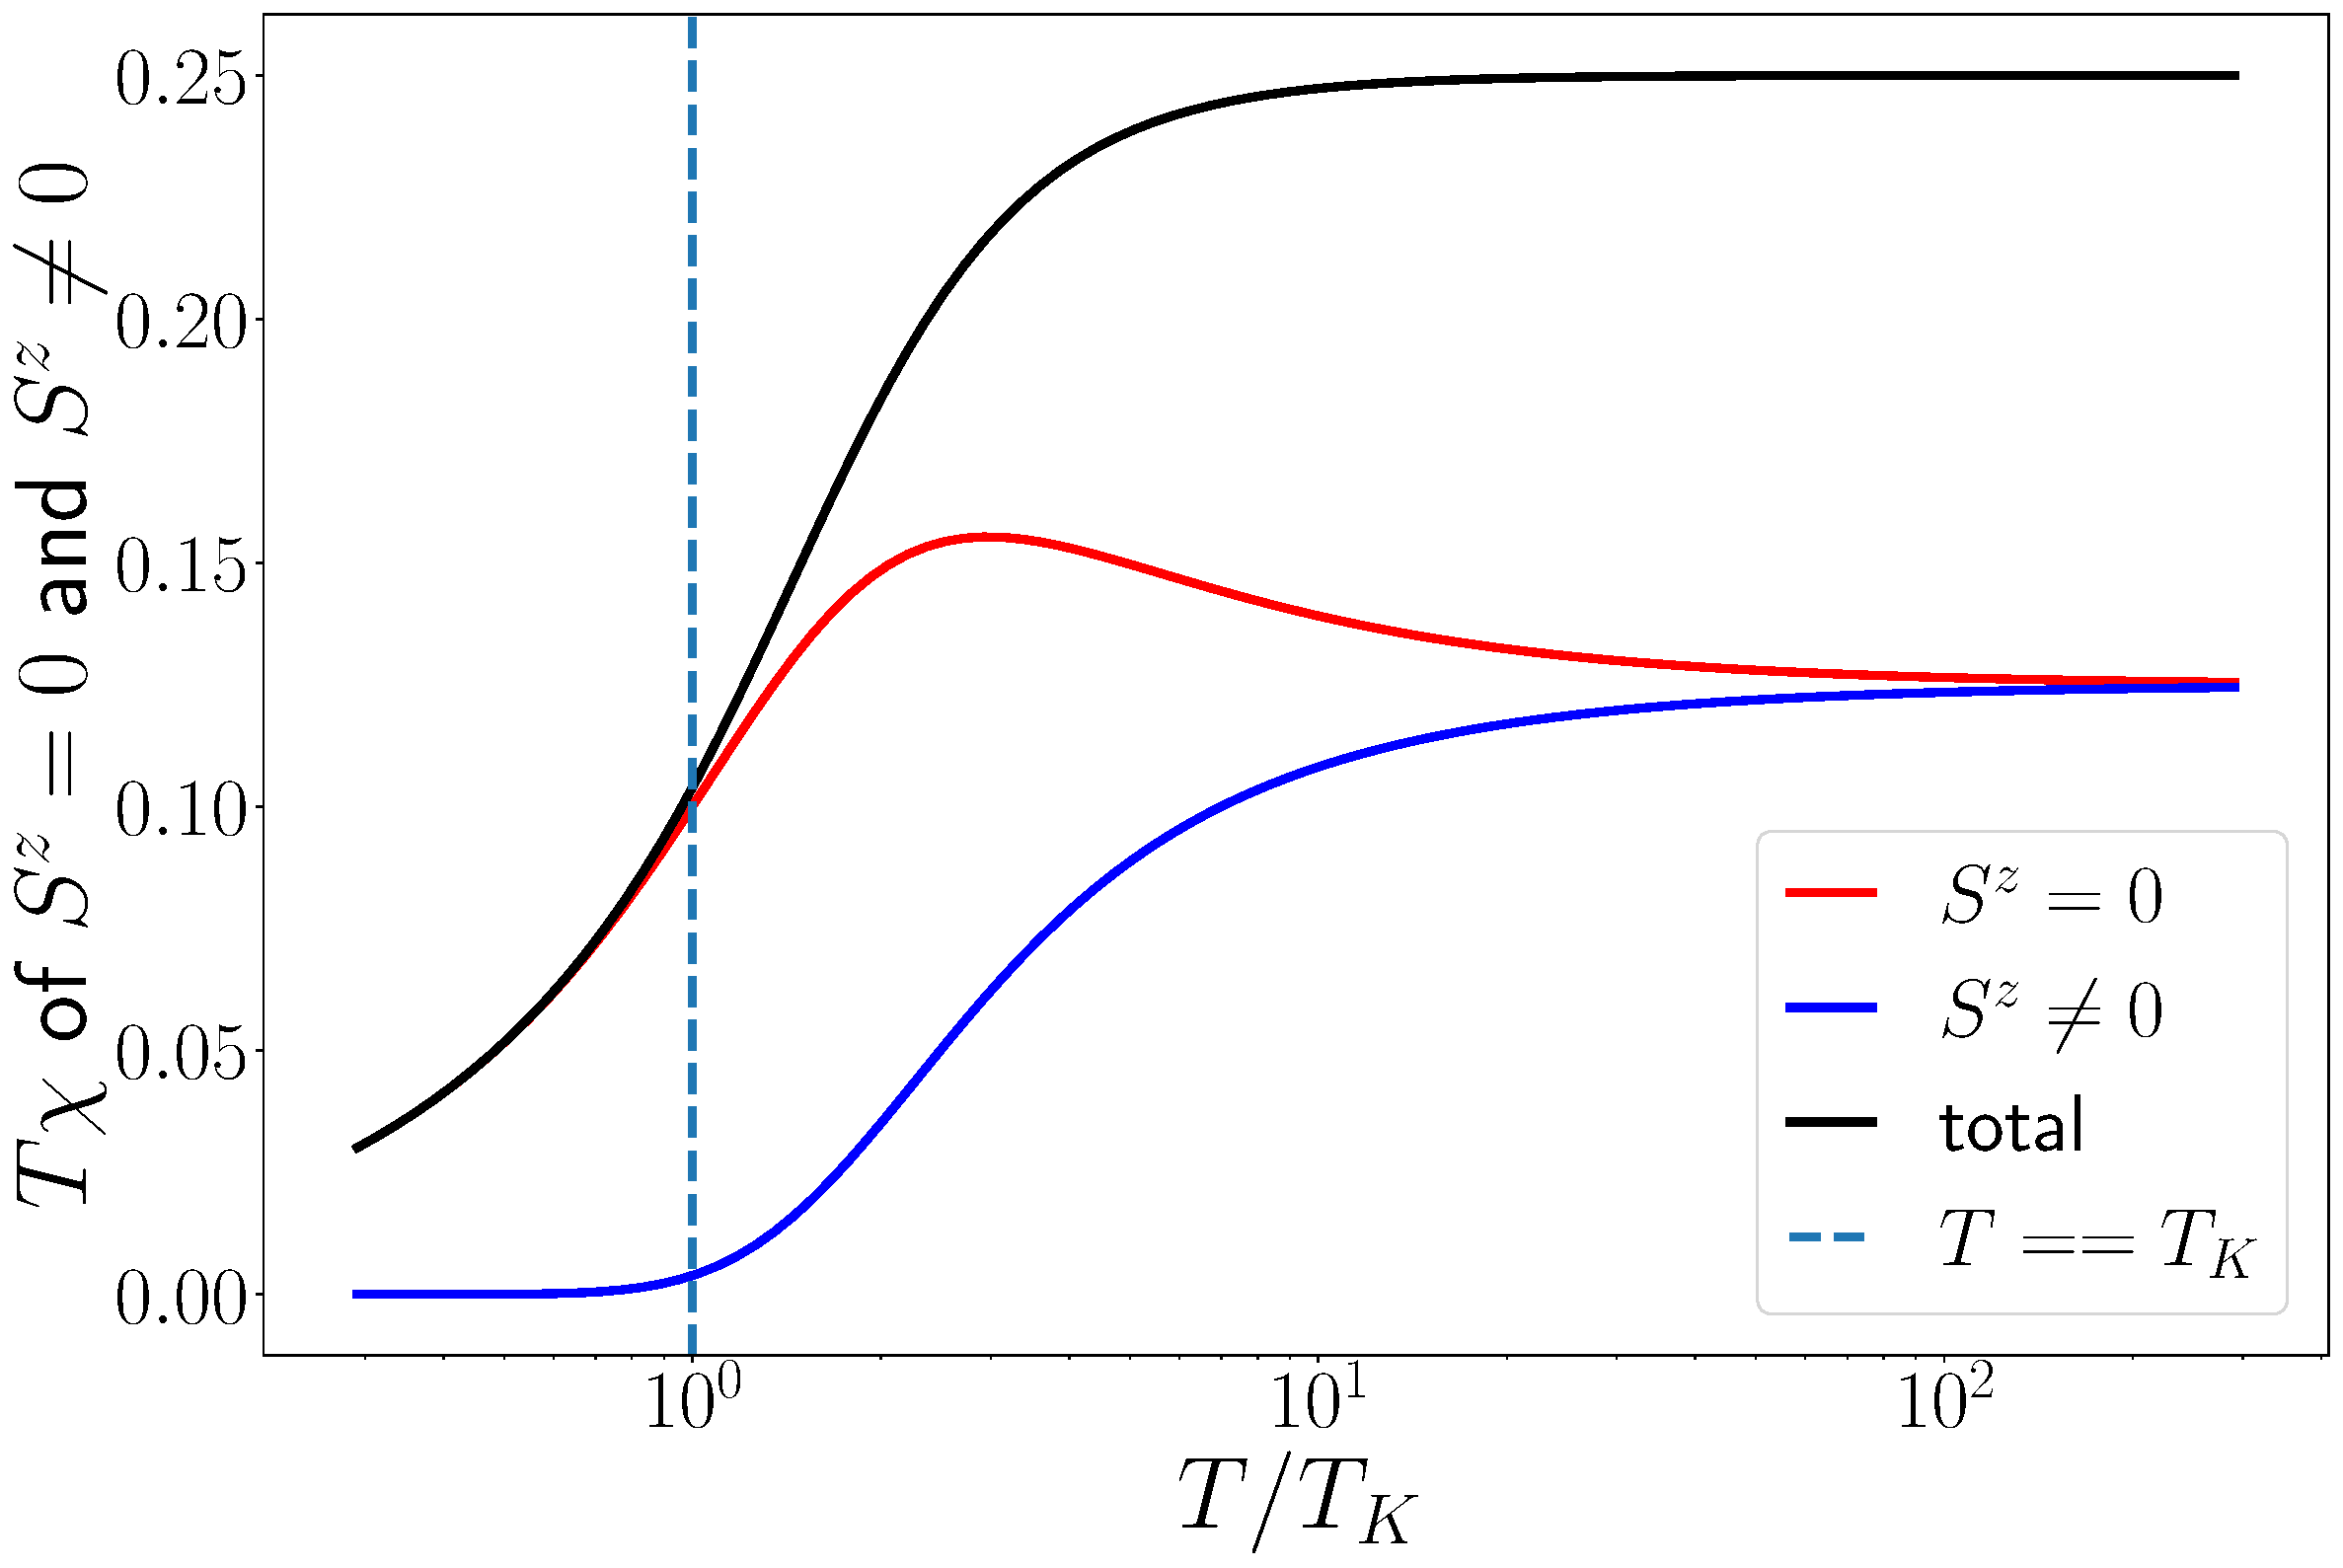
\includegraphics[width=0.95\textwidth]{figures/chi_times_T_parts.pdf}
\vspace*{-20pt}
}
\only<4>{
\[\chi(T \to 0) = \frac{1}{2 J^*}, ~ ~ 4 T_K \chi(T \to 0) = W \sim 0.413\]
\focus{LM is screened} ~ ~ \(W=\)Wilson number
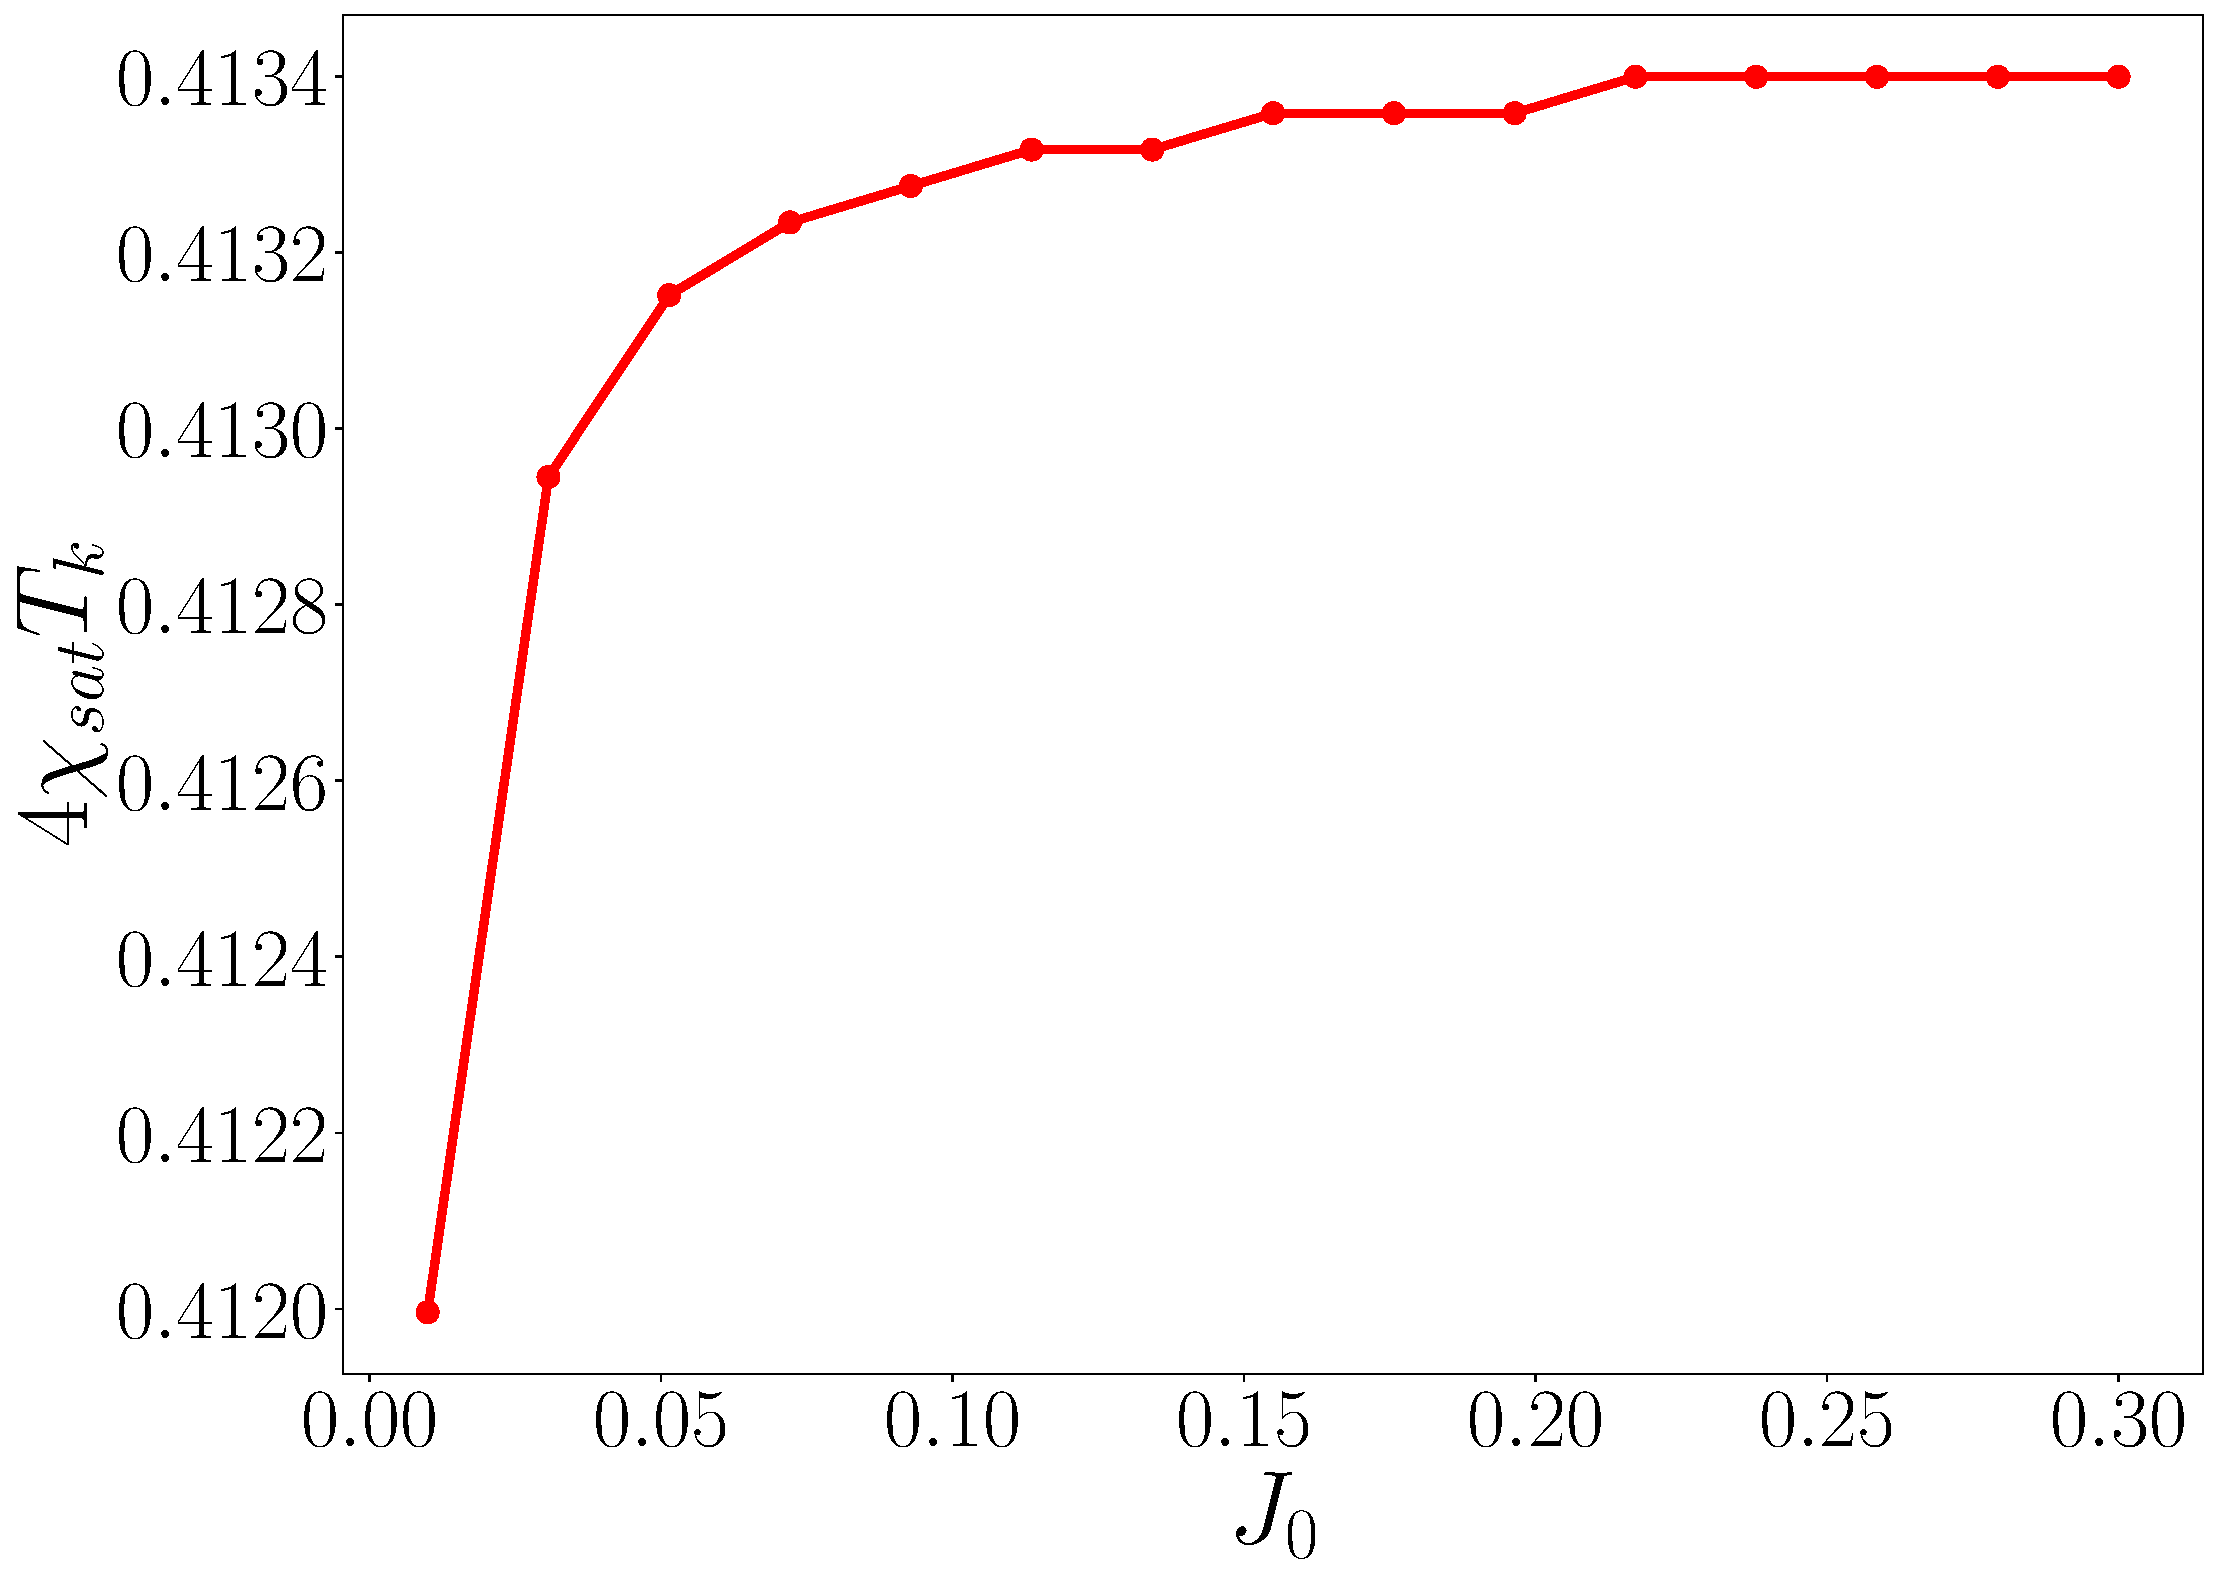
\includegraphics[width=0.85\textwidth]{figures/WilsonNumber.pdf}
\vspace*{-20pt}
}
\only<5>{
\focus{Maximum in \(\chi\) at \(T_K\)}

Contribution from polarised states vanish
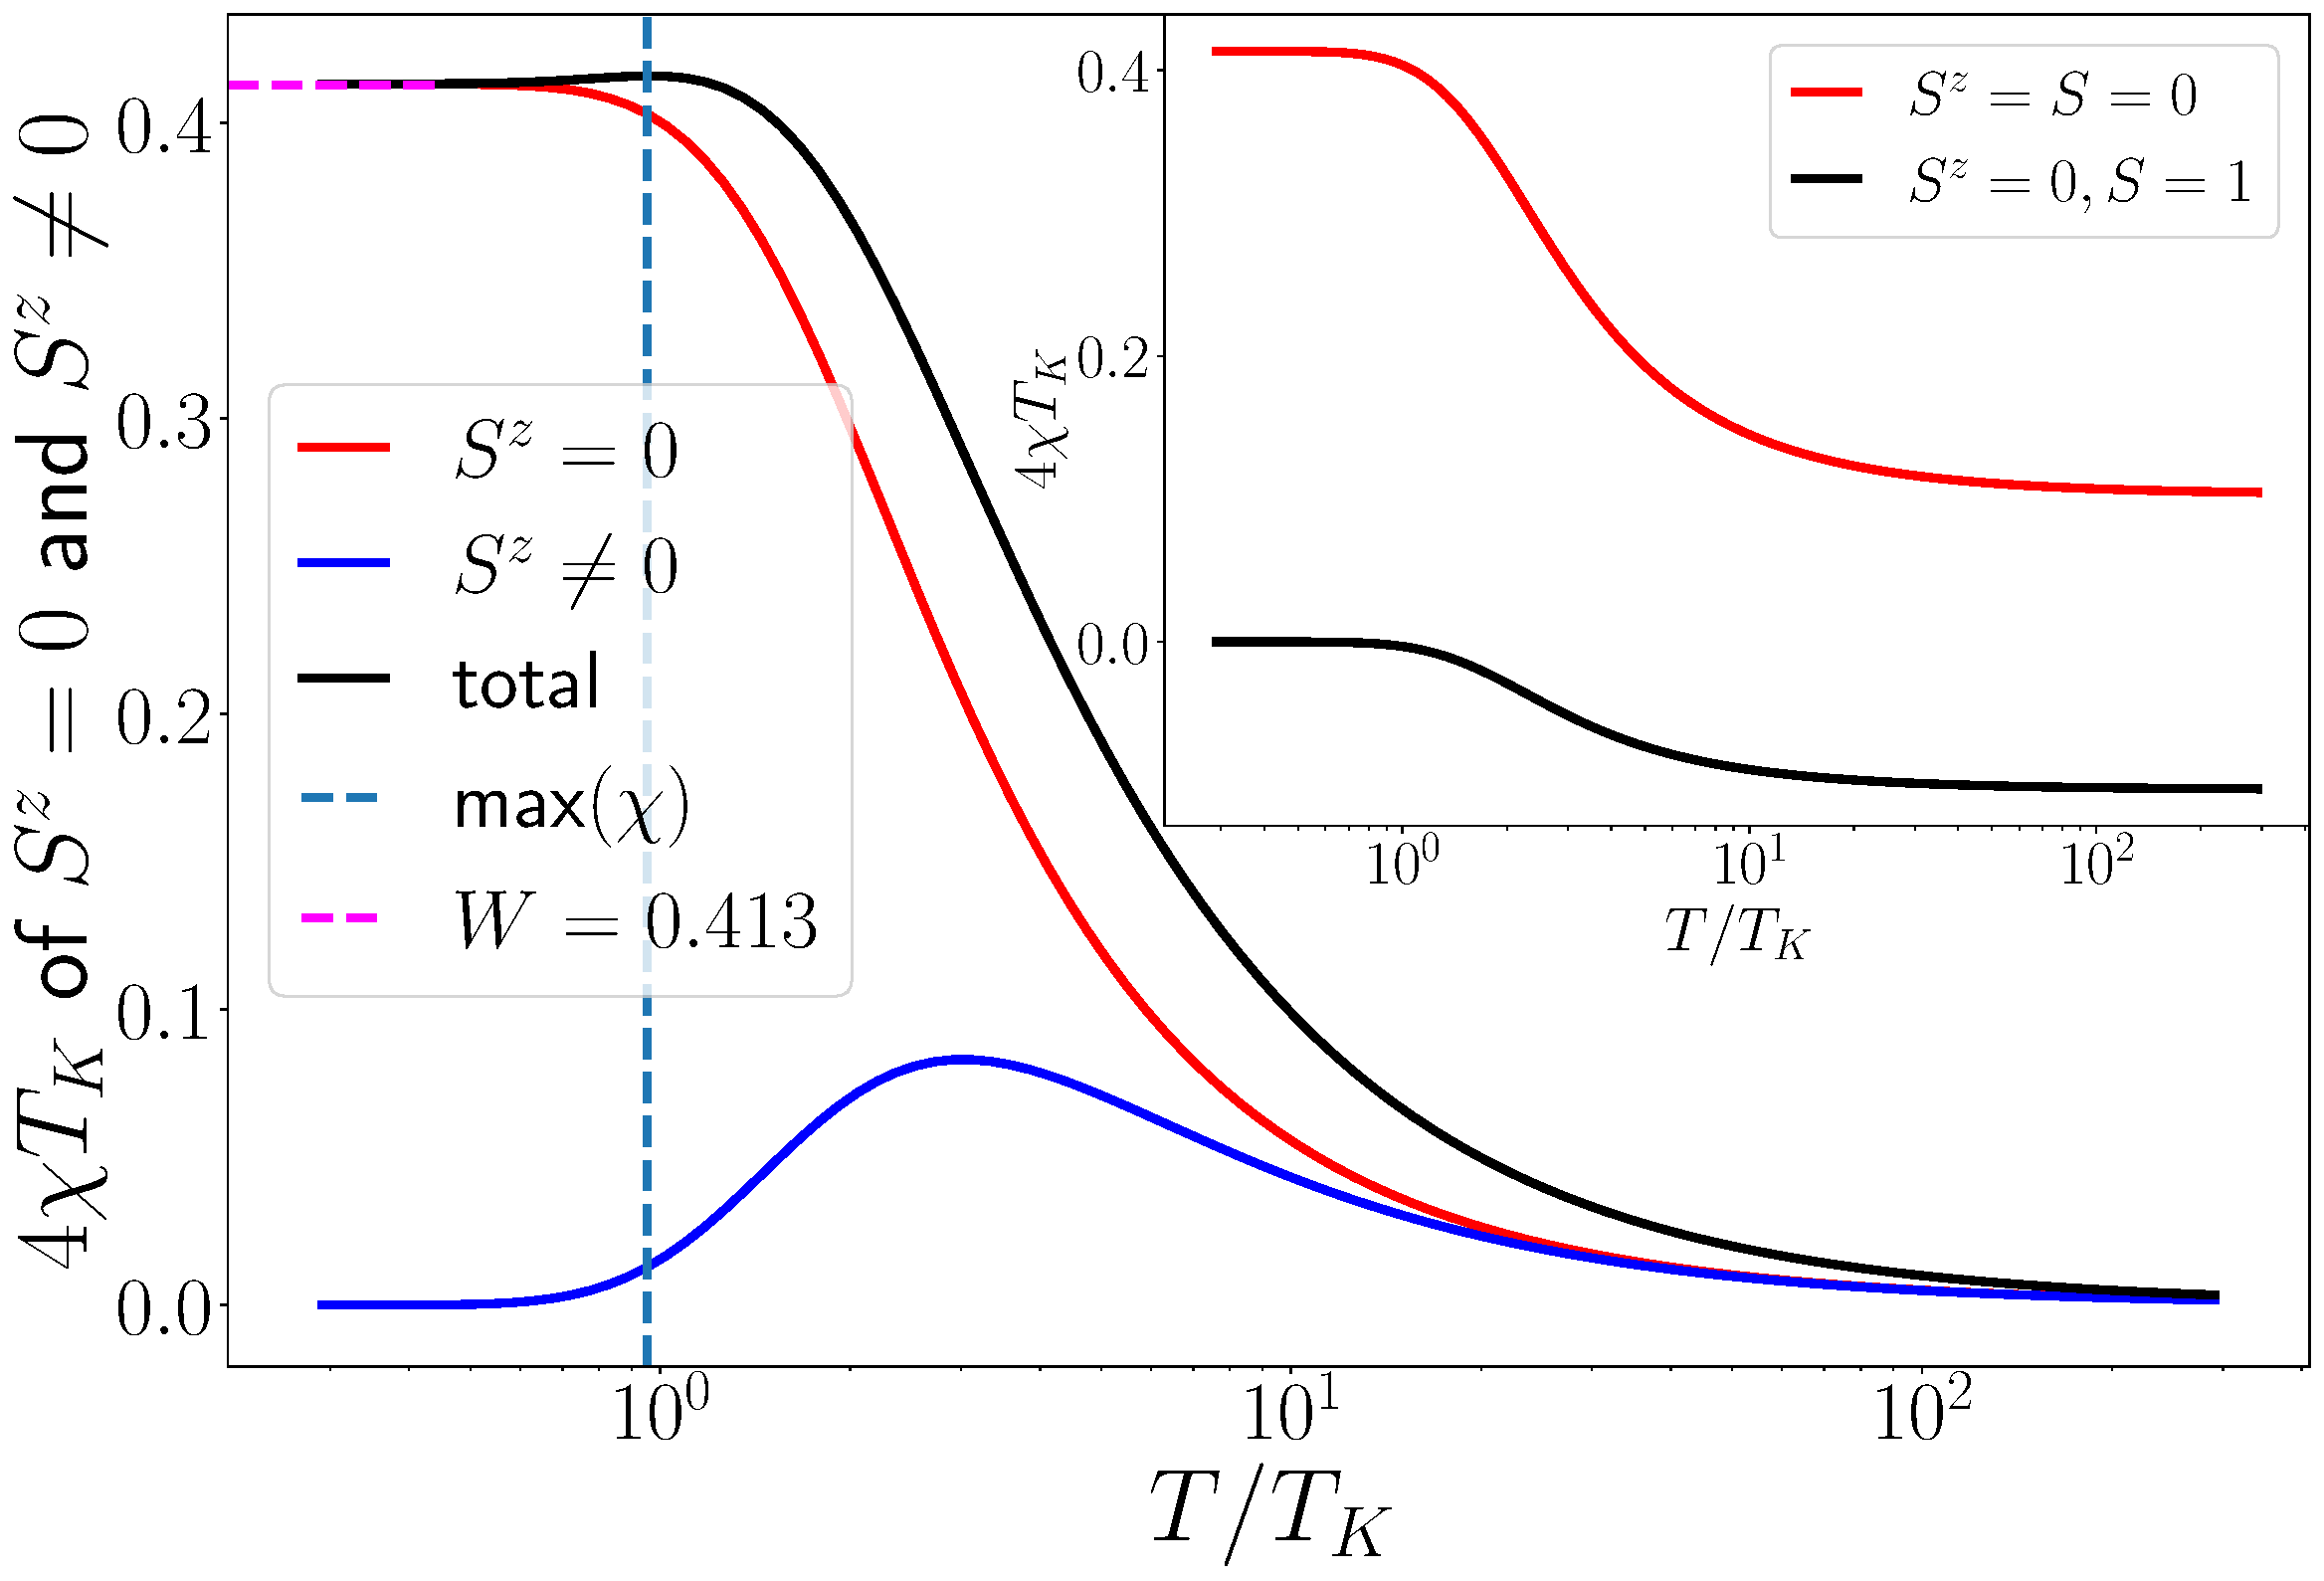
\includegraphics[width=1.05\textwidth]{figures/chi_parts.pdf}
\vspace*{-40pt}
}
\end{minipage}
}

\only<3>{
	\begin{textblock*}{\textwidth}(0pt, 0.85\textheight)
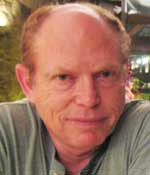
\includegraphics[height=40pt]{figures/andrei.jpg}
\end{textblock*}
}
\end{frame}

\section{Effective Hamiltonian for the Kondo Cloud}
\begin{frame}[noframenumbering]{Effective Hamiltonian for the Kondo Cloud}
	\only<1-3>{
	\begin{itemize}
	\only<+->{	\item Restore the kinetic energy part:

			\[H^* = \sum_{k < k^*,\sigma}\epsilon_{k}\hat{n}_{k\sigma} ~ + ~ J^* \vec{S}_d\cdot \vec{s}_< = \underbrace{\sum_{k < k^*,\sigma}\epsilon_{k}\hat{n}_{k\sigma} ~ + ~ J^* S_d^z s_<^z}_{H_D} ~+~ \underbrace{J^*{S}_d^+ {s}_<^- + \text{h.c.}}_{V ~+~ V^\dagger}\]}

 	\only<+->{	\item Freeze impurity dynamics by integrating out \(V\)\footcite{hewson1993}:

			\[H_\text{eff} = H_D + V \frac{1}{E_\text{gs} - H_D} V^\dagger + V^\dagger \frac{1}{E_\text{gs} - H_D} V\]}

\only<+->{
\item Resolve \(k-\)space part by expanding denominator in \(\epsilon_k/E_\text{gs}\):

\[V \frac{1}{E_\text{gs} - H_D} V^\dagger = V \left(\frac{1}{E_\text{gs}} + \frac{H_D}{E_\text{gs}^2} + \ldots\right) \]}
\end{itemize}

}
\only<2-3>{
\begin{textblock*}{\textwidth}(0.95\textwidth, 0.85\textheight)
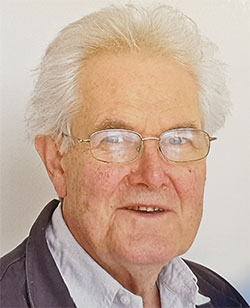
\includegraphics[height=40pt]{figures/hewson.jpg}
\end{textblock*}
}
\only<4>{
\head{Form of Kondo cloud Hamiltonian}
\centering
\[H_\text{eff}=2H^{*}_{0} ~+~ \frac{2}{J^*}{H^{*}_{0}}^2 ~+~ \sum_{1234}V_{1234}c^\dagger_{{k_4} \uparrow}c^\dagger_{{k_3} \downarrow}c_{{k_2} \downarrow}c_{{k_1} \uparrow}\label{eff_Ham_Kondo}\]
\[V_{1234} = \left( \epsilon_{k_1} - \epsilon_{k_3} \right)\left[1 - \frac{2}{J^*}\left(\epsilon_{k_3} - \epsilon_{{k_1}} + \epsilon_{{k_2}} + \epsilon_{{k_4}}\right)\right]\]

\begin{itemize}
	\item Mixture of \focus{Fermi liquid} and \focus{two-particle off-diagonal scattering term}
		\vspace*{\fill}
	\item Fermi liquid part: \focus{result of Ising scattering}
		\vspace*{\fill}
	\item 2P off-diagonal term: \focus{Non-Fermi liquid} in character - \focus{result of spin-flip scattering}
		\vspace*{\fill}
	\item NFL part \focus{leads to screening} and formation of singlet
\end{itemize}
}

\only<5-6>{
\head{Impurity specific heat}
\begin{minipage}{0.5\textwidth}
\begin{itemize}
	\item Fermi-liquid part renormalises one-particle \focus{self-energy}
		\[\bar{\epsilon}_{k}=\epsilon_{k}+\Sigma_{k}\]
	\[\Sigma_{k}=\sum_{k^\prime\sigma^\prime}\frac{\epsilon_{k^\prime}\epsilon_{k}}{J^{*}}\delta n_{k^\prime,\sigma^\prime}\]
	\only<6>{\item Compute renormalisation in \(C_V\):
		\[
C_\text{imp} = \sum_{k,\sigma}\frac{1}{T^2}\left[\frac{(\bar{\epsilon}_{k})^{2}e^{\beta\bar{\epsilon}_{k}}}{(e^{\beta\bar{\epsilon}_{k}}+1)^{2}}-\frac{(\epsilon_{k})^{2}e^{\beta\epsilon_{k}}}{(e^{\beta\epsilon_{k}}+1)^{2}}\right]
\]
}
\end{itemize}
\end{minipage}
\only<5>{
\begin{minipage}{0.48\textwidth}
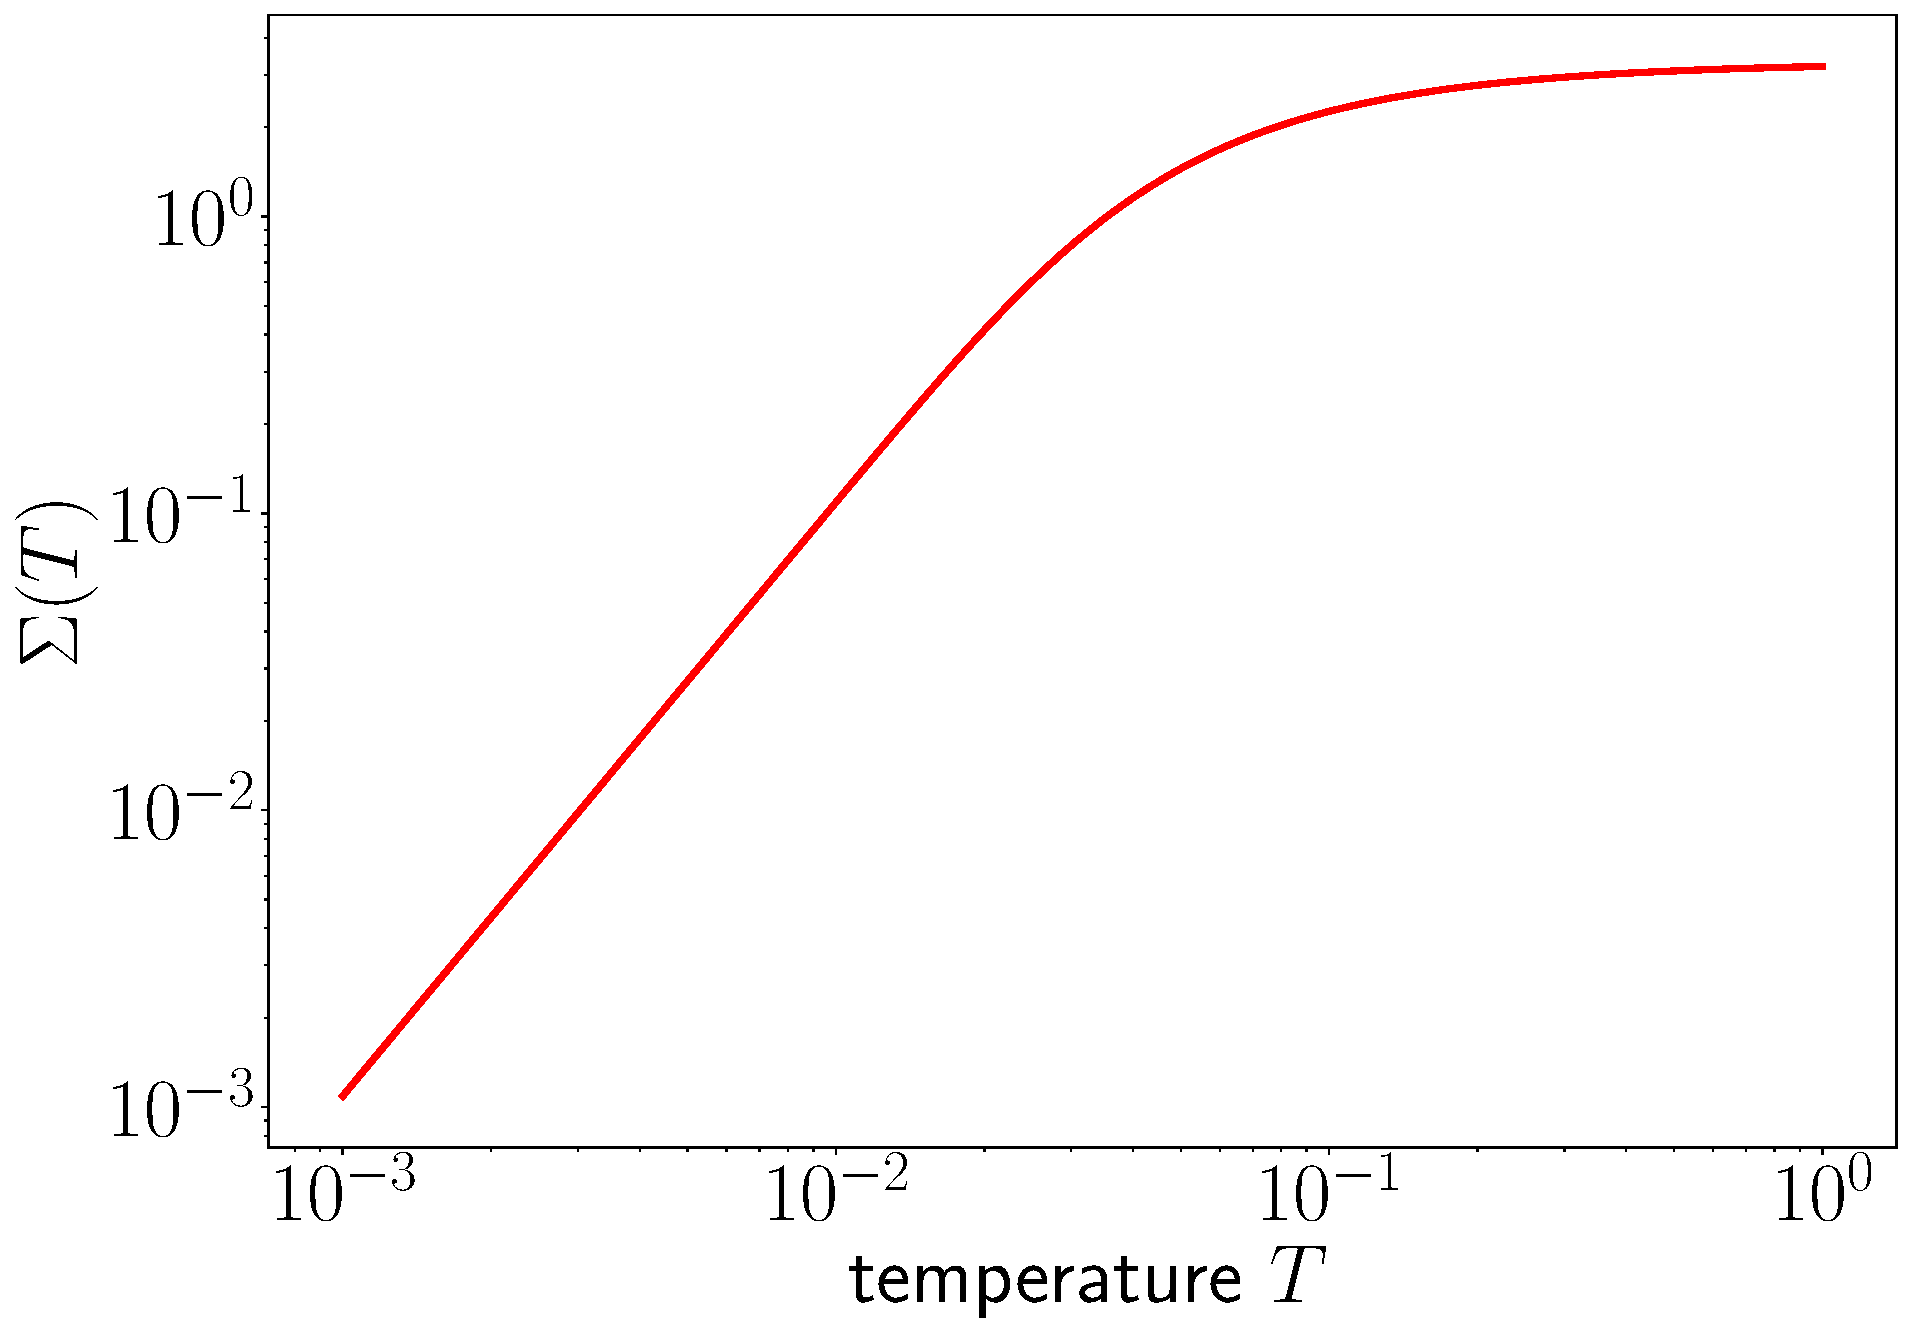
\includegraphics[width=\textwidth]{figures/FL_self_energy.pdf}
\end{minipage}
}
\only<6>{
\footcite{wilson1975,andrei_kondo,wiegmann_kondoexact_1981}
\begin{minipage}{0.48\textwidth}
	\[ C_V = \gamma \times T\]
	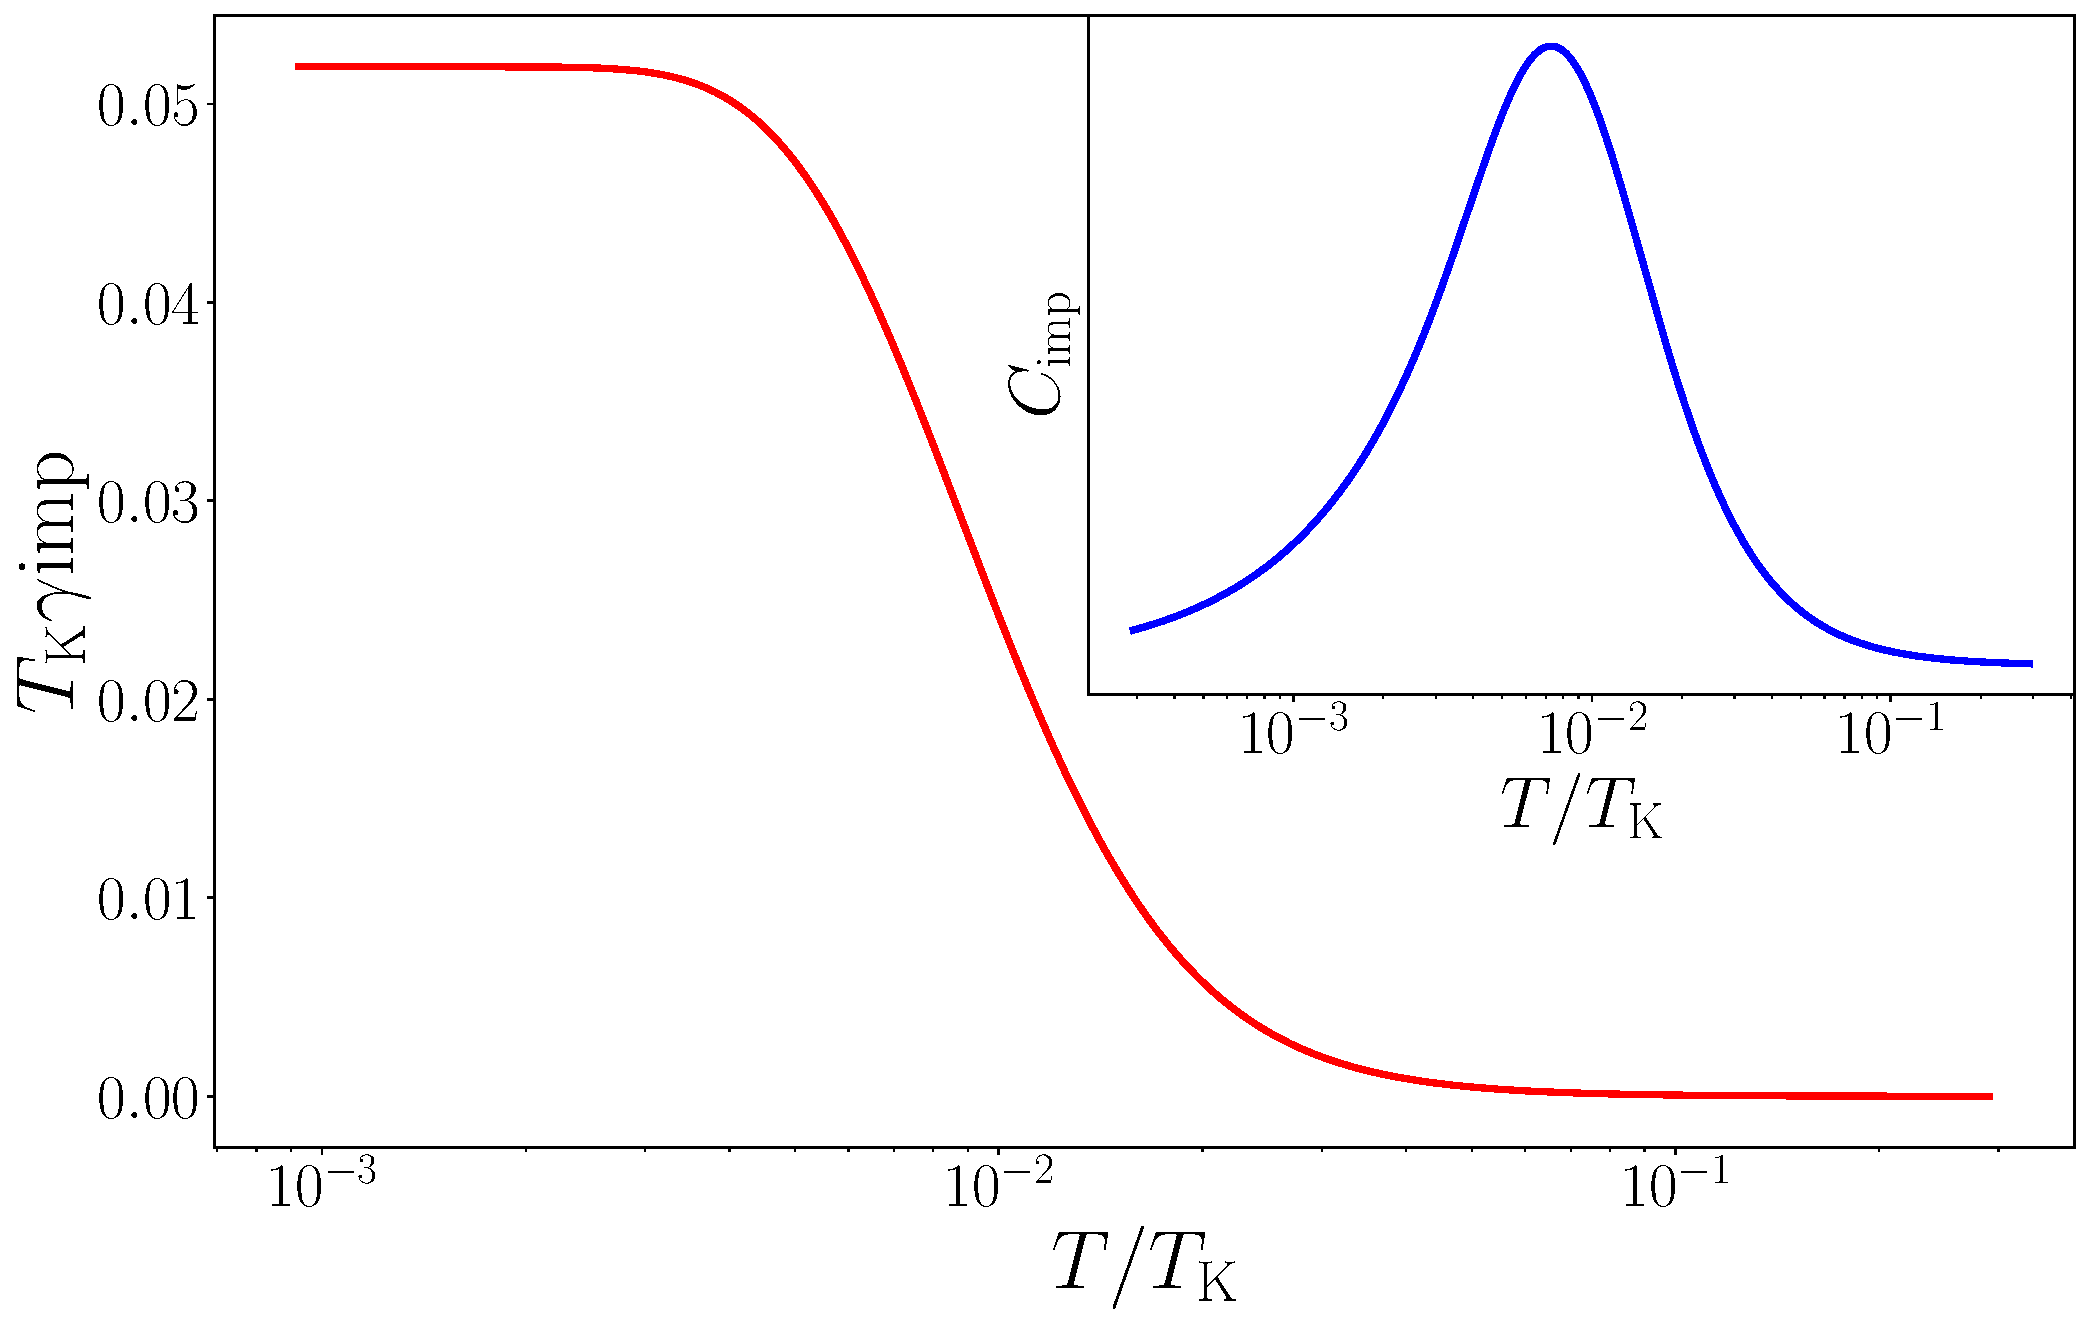
\includegraphics[width=\textwidth]{figures/gamma_imp.pdf}
\end{minipage}
}
}
\only<7>{
\head{Wilson ratio}
\footcite{wilson1975,andrei_kondo,wiegmann_kondoexact_1981}

\begin{minipage}{0.35\textwidth}
\begin{flushleft}
	\(R = \frac{\chi}{\gamma}\)\\[15pt]
	\(\chi(T \to 0) = \frac{1}{2J^*}\)\\[15pt]
	\(\gamma(T \to 0) = \frac{1}{4J^*}\)\\[15pt]
	\focus{\(R\) saturates to 2 as \(T \to 0\)}
\end{flushleft}
\end{minipage}
\hspace*{\fill}
\begin{minipage}{0.6\textwidth}
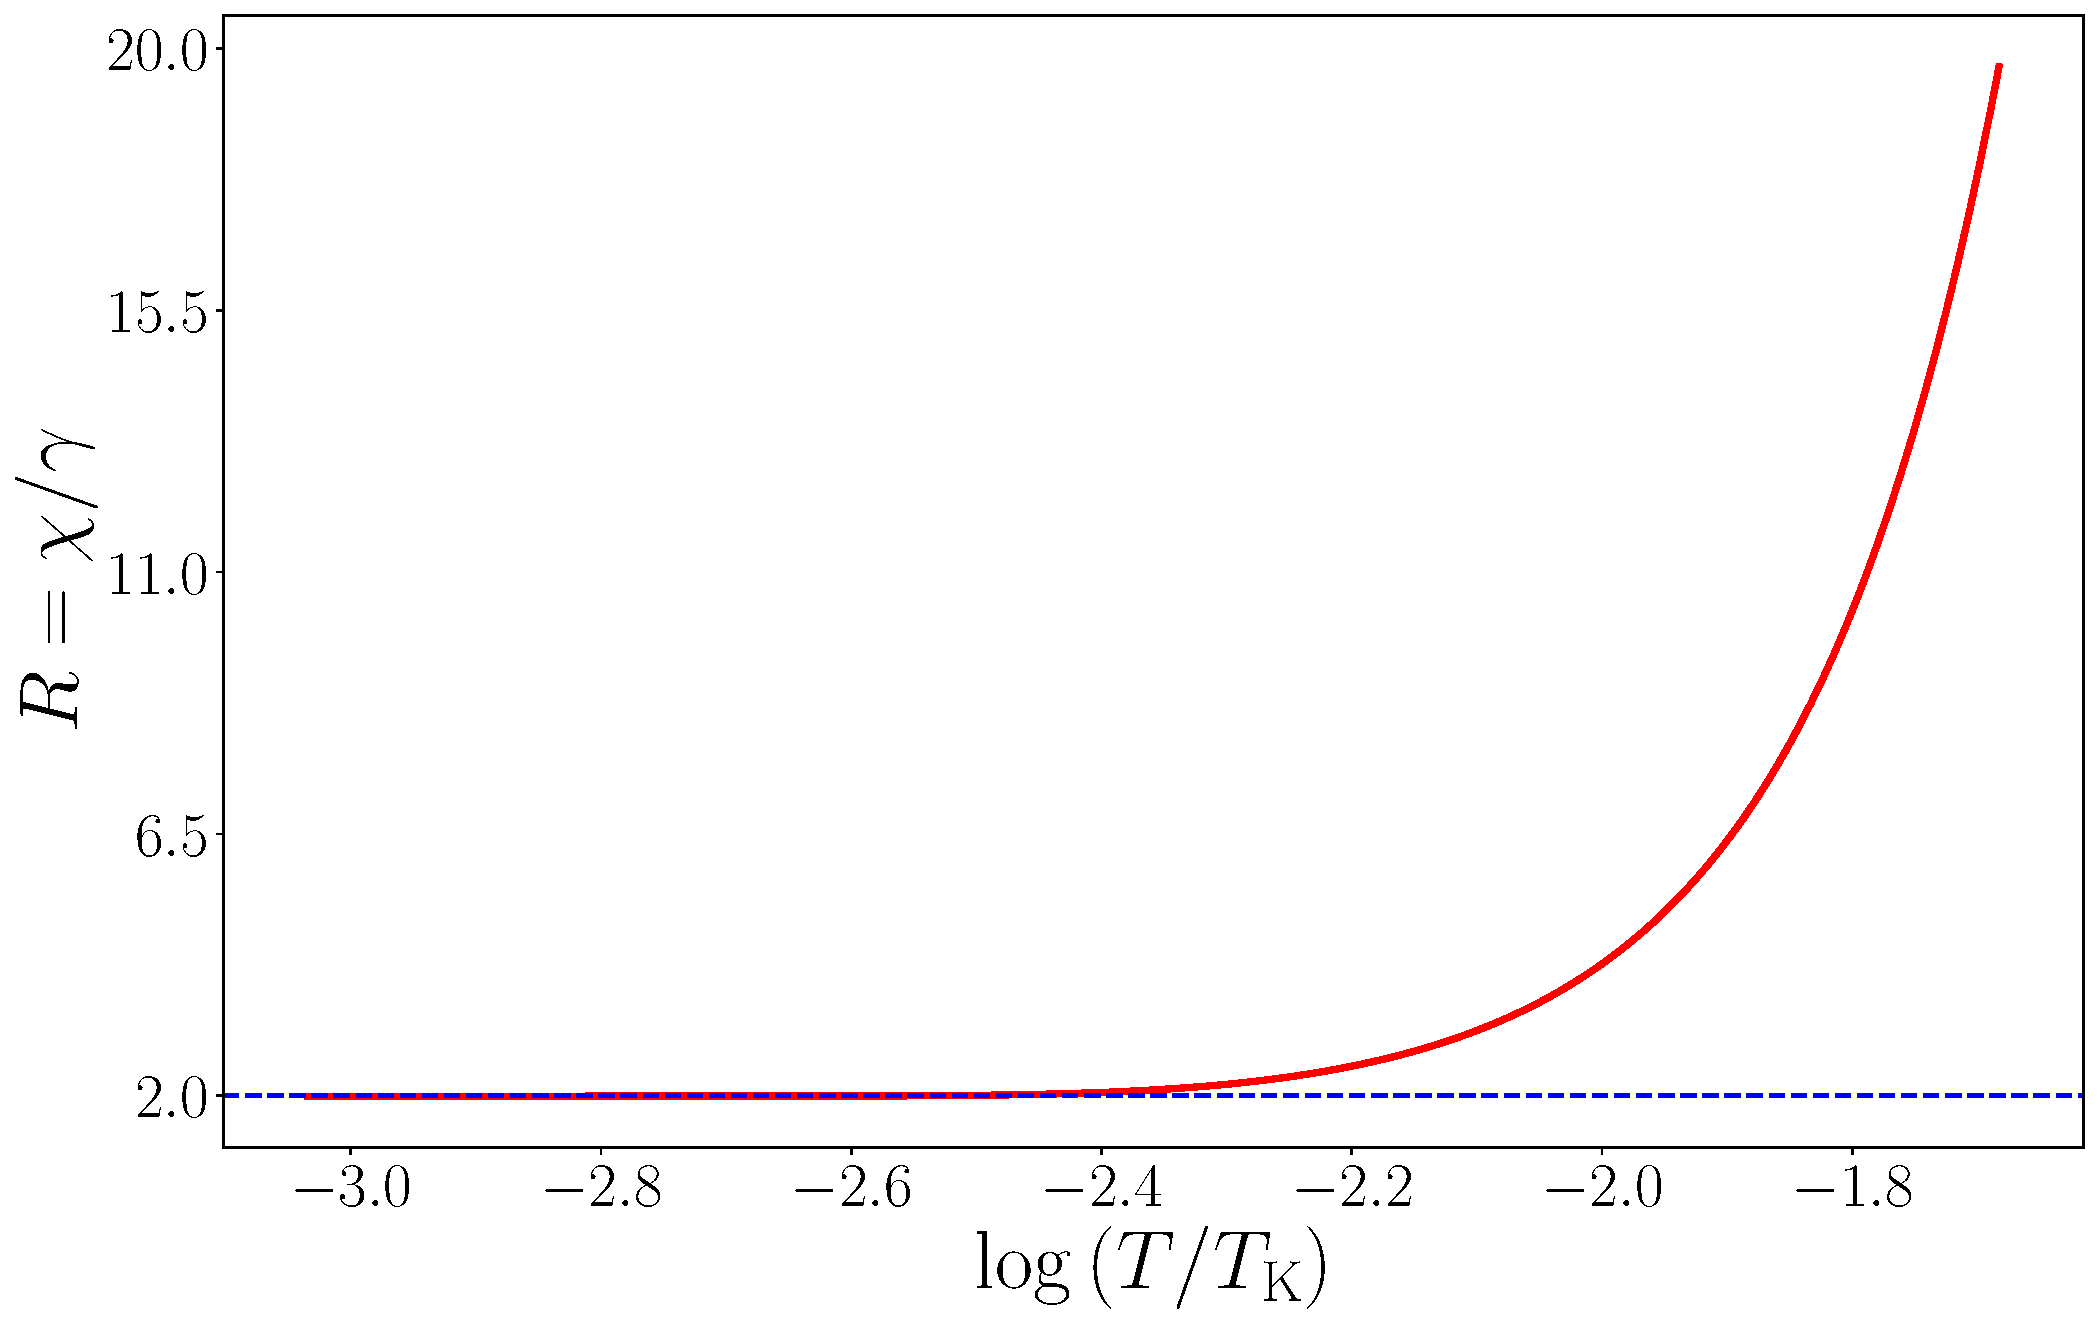
\includegraphics[width=0.9\textwidth]{figures/wilsonratio.pdf}
\end{minipage}
}
\end{frame}

\section{Many-particle entanglement \& many-body correlation}
\begin{frame}[noframenumbering]{Many-particle entanglement \& many-body correlation}

\only<1-3>{\footcite{siddharthacpi,1dhubjhep}}
\only<1>{
\head{Reverse RG: What does it mean?}
	\centering
	\begin{itemize}
		\item \focus{retrace RG flow} by applying \focus{inverse unitary transformations} on ground state

	\end{itemize}

	\vspace*{\fill}

	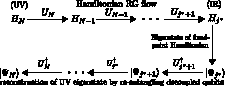
\includegraphics[width=0.6\textwidth]{figures/flowChart_new.pdf}
	% \end{minipage}
}

\only<2-3>{
\head{Reverse RG: Algorithm}
\centering
\begin{minipage}{0.68\textwidth}
\begin{itemize}
	\item Start with \focus{minimal IR ground state}:
		\[\ket{\Psi}_0 = \ket{\text{singlet}}\otimes\ket{\text{IOMs}}\]
\end{itemize}
\end{minipage}
\begin{minipage}{0.3\textwidth}
	\centering
	\only<2-3>{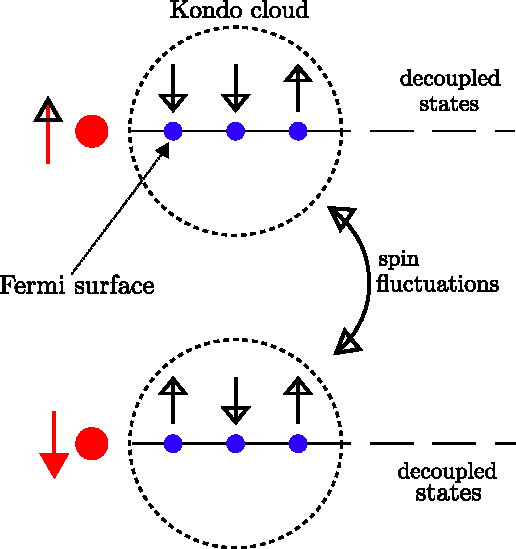
\includegraphics[width=\textwidth]{figures/KC.pdf}}
\end{minipage}

\only<3>{
\begin{minipage}{0.68\textwidth}
\begin{itemize}
	\item \focus{Re-entangle} \(\ket{\Psi}_0\) with IOMs:
		\[ \ket{\Psi}_1 = U^\dagger_0 \ket{\Psi}_0\]
		\[
		U_{q\sigma}^{-1} = \frac{1}{\sqrt 2}\left[ 1 - \frac{J^2}{2}\frac{1}{2\omega \tau_{q\sigma} - \epsilon_{q}\tau_{q\sigma} - J S^z s^z_q}\left(\hat O + {\hat O}^\dagger\right)\right]\]
		\[\hat O = \sum_{k < \Lambda^*}\sum_{\alpha=\uparrow, \downarrow} \sum_{a={x,y,z}}S^a\sigma^a_{\alpha\sigma}c^\dagger_{k\alpha}c_{q\sigma}\]
\end{itemize}
\end{minipage}
\hspace*{\fill}
\begin{minipage}{0.3\textwidth}
	\centering
	\only<3>{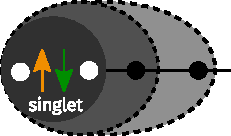
\includegraphics[width=\textwidth]{figures/KC_2.pdf}}
\end{minipage}

}
}

\only<4-5>{
\head{Entanglement and Correlation along RG Flow}
\only<4>{
\begin{minipage}{0.45\textwidth}
	\centering
	\focus{Mutual Information}
	\[ I(i:j)=S_i + S_j - S_{ij}\]
	\[ S_i = \text{Tr} \left(\rho_i \ln \rho_i\right),  S_{ij} = \text{Tr} \left(\rho_{ij} \ln \rho_{ij}\right)\]\\[10pt]
	\begin{itemize}
		\item MI between imp. and a \(k\)-state\\[10pt]
		\item MI between \(k\)-states\\[10pt]
	\end{itemize}

	\focus{Both increase towards IR}
\end{minipage}
\begin{minipage}{0.54\textwidth}
	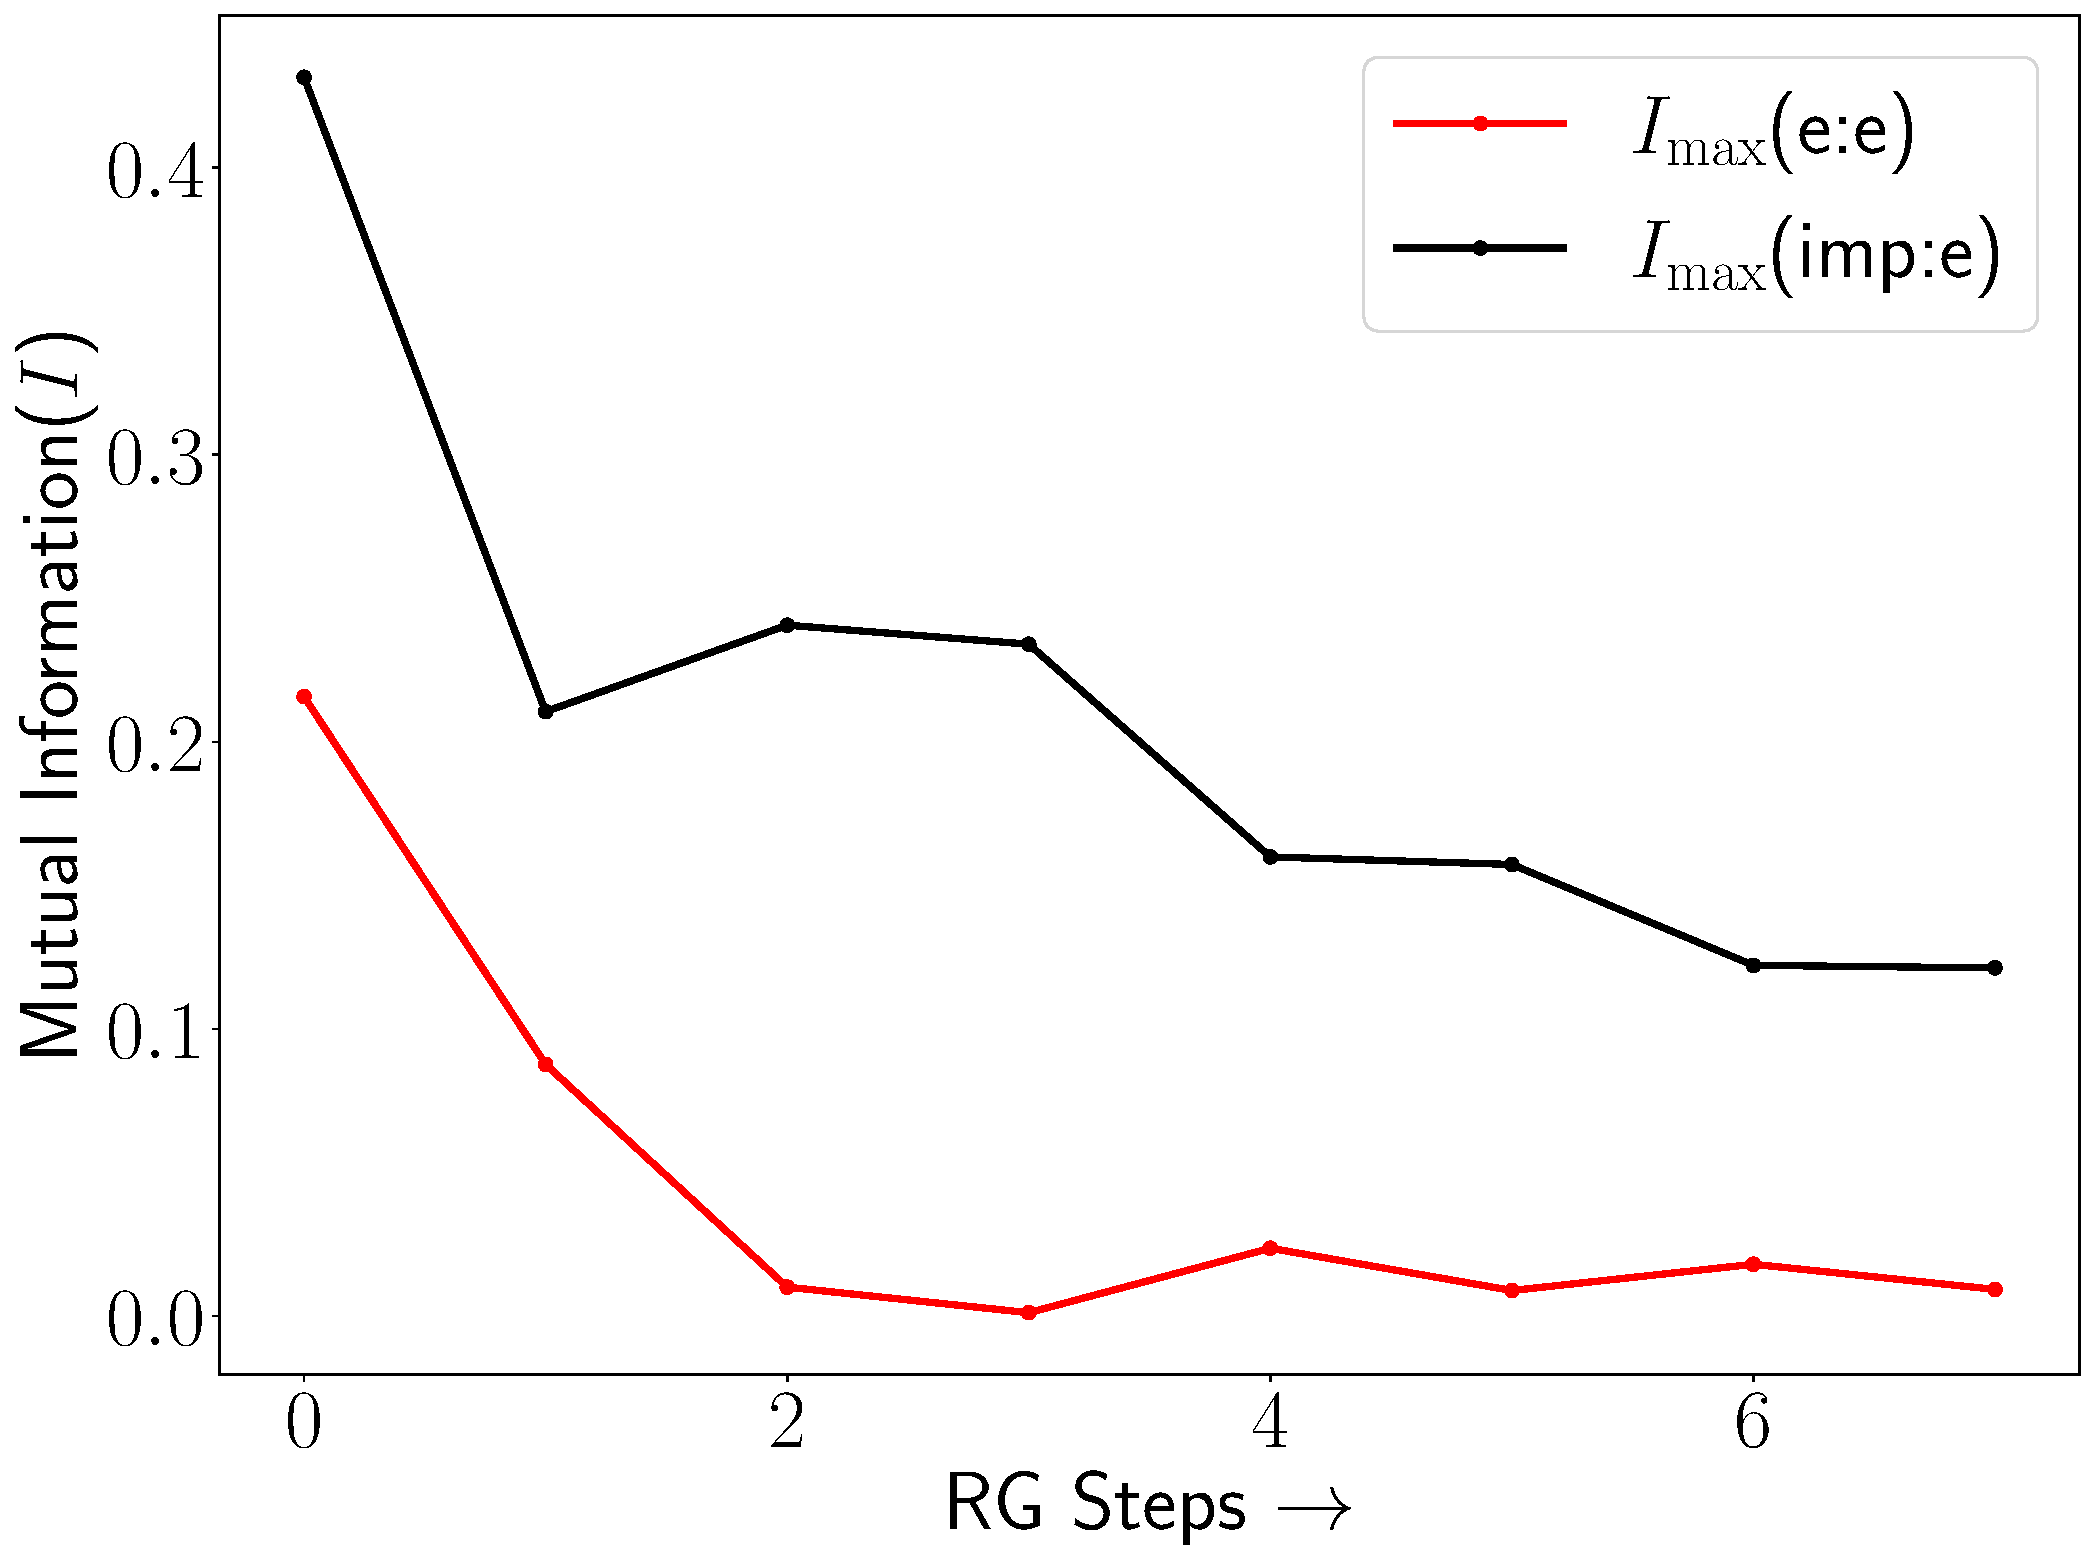
\includegraphics[width=\textwidth]{figures/MIkondo.pdf}
\end{minipage}
}
\only<5>{
\begin{minipage}{0.45\textwidth}
	\centering
	\focus{Correlations}
	\\[10pt]
	\begin{itemize}
		\item Diagonal correlation \(\left<\hat n_{1 \uparrow} \hat n_{2 \uparrow} \right>\)\\[10pt]
		\item 2-particle off-diagonal correlation \(\left<c^\dagger_{1\uparrow}c^\dagger_{2\downarrow}c_{3\downarrow}c_{1\uparrow} \right>\)\\[10pt]
	\end{itemize}
	\focus{Both increase towards IR}
\end{minipage}
\begin{minipage}{0.54\textwidth}
	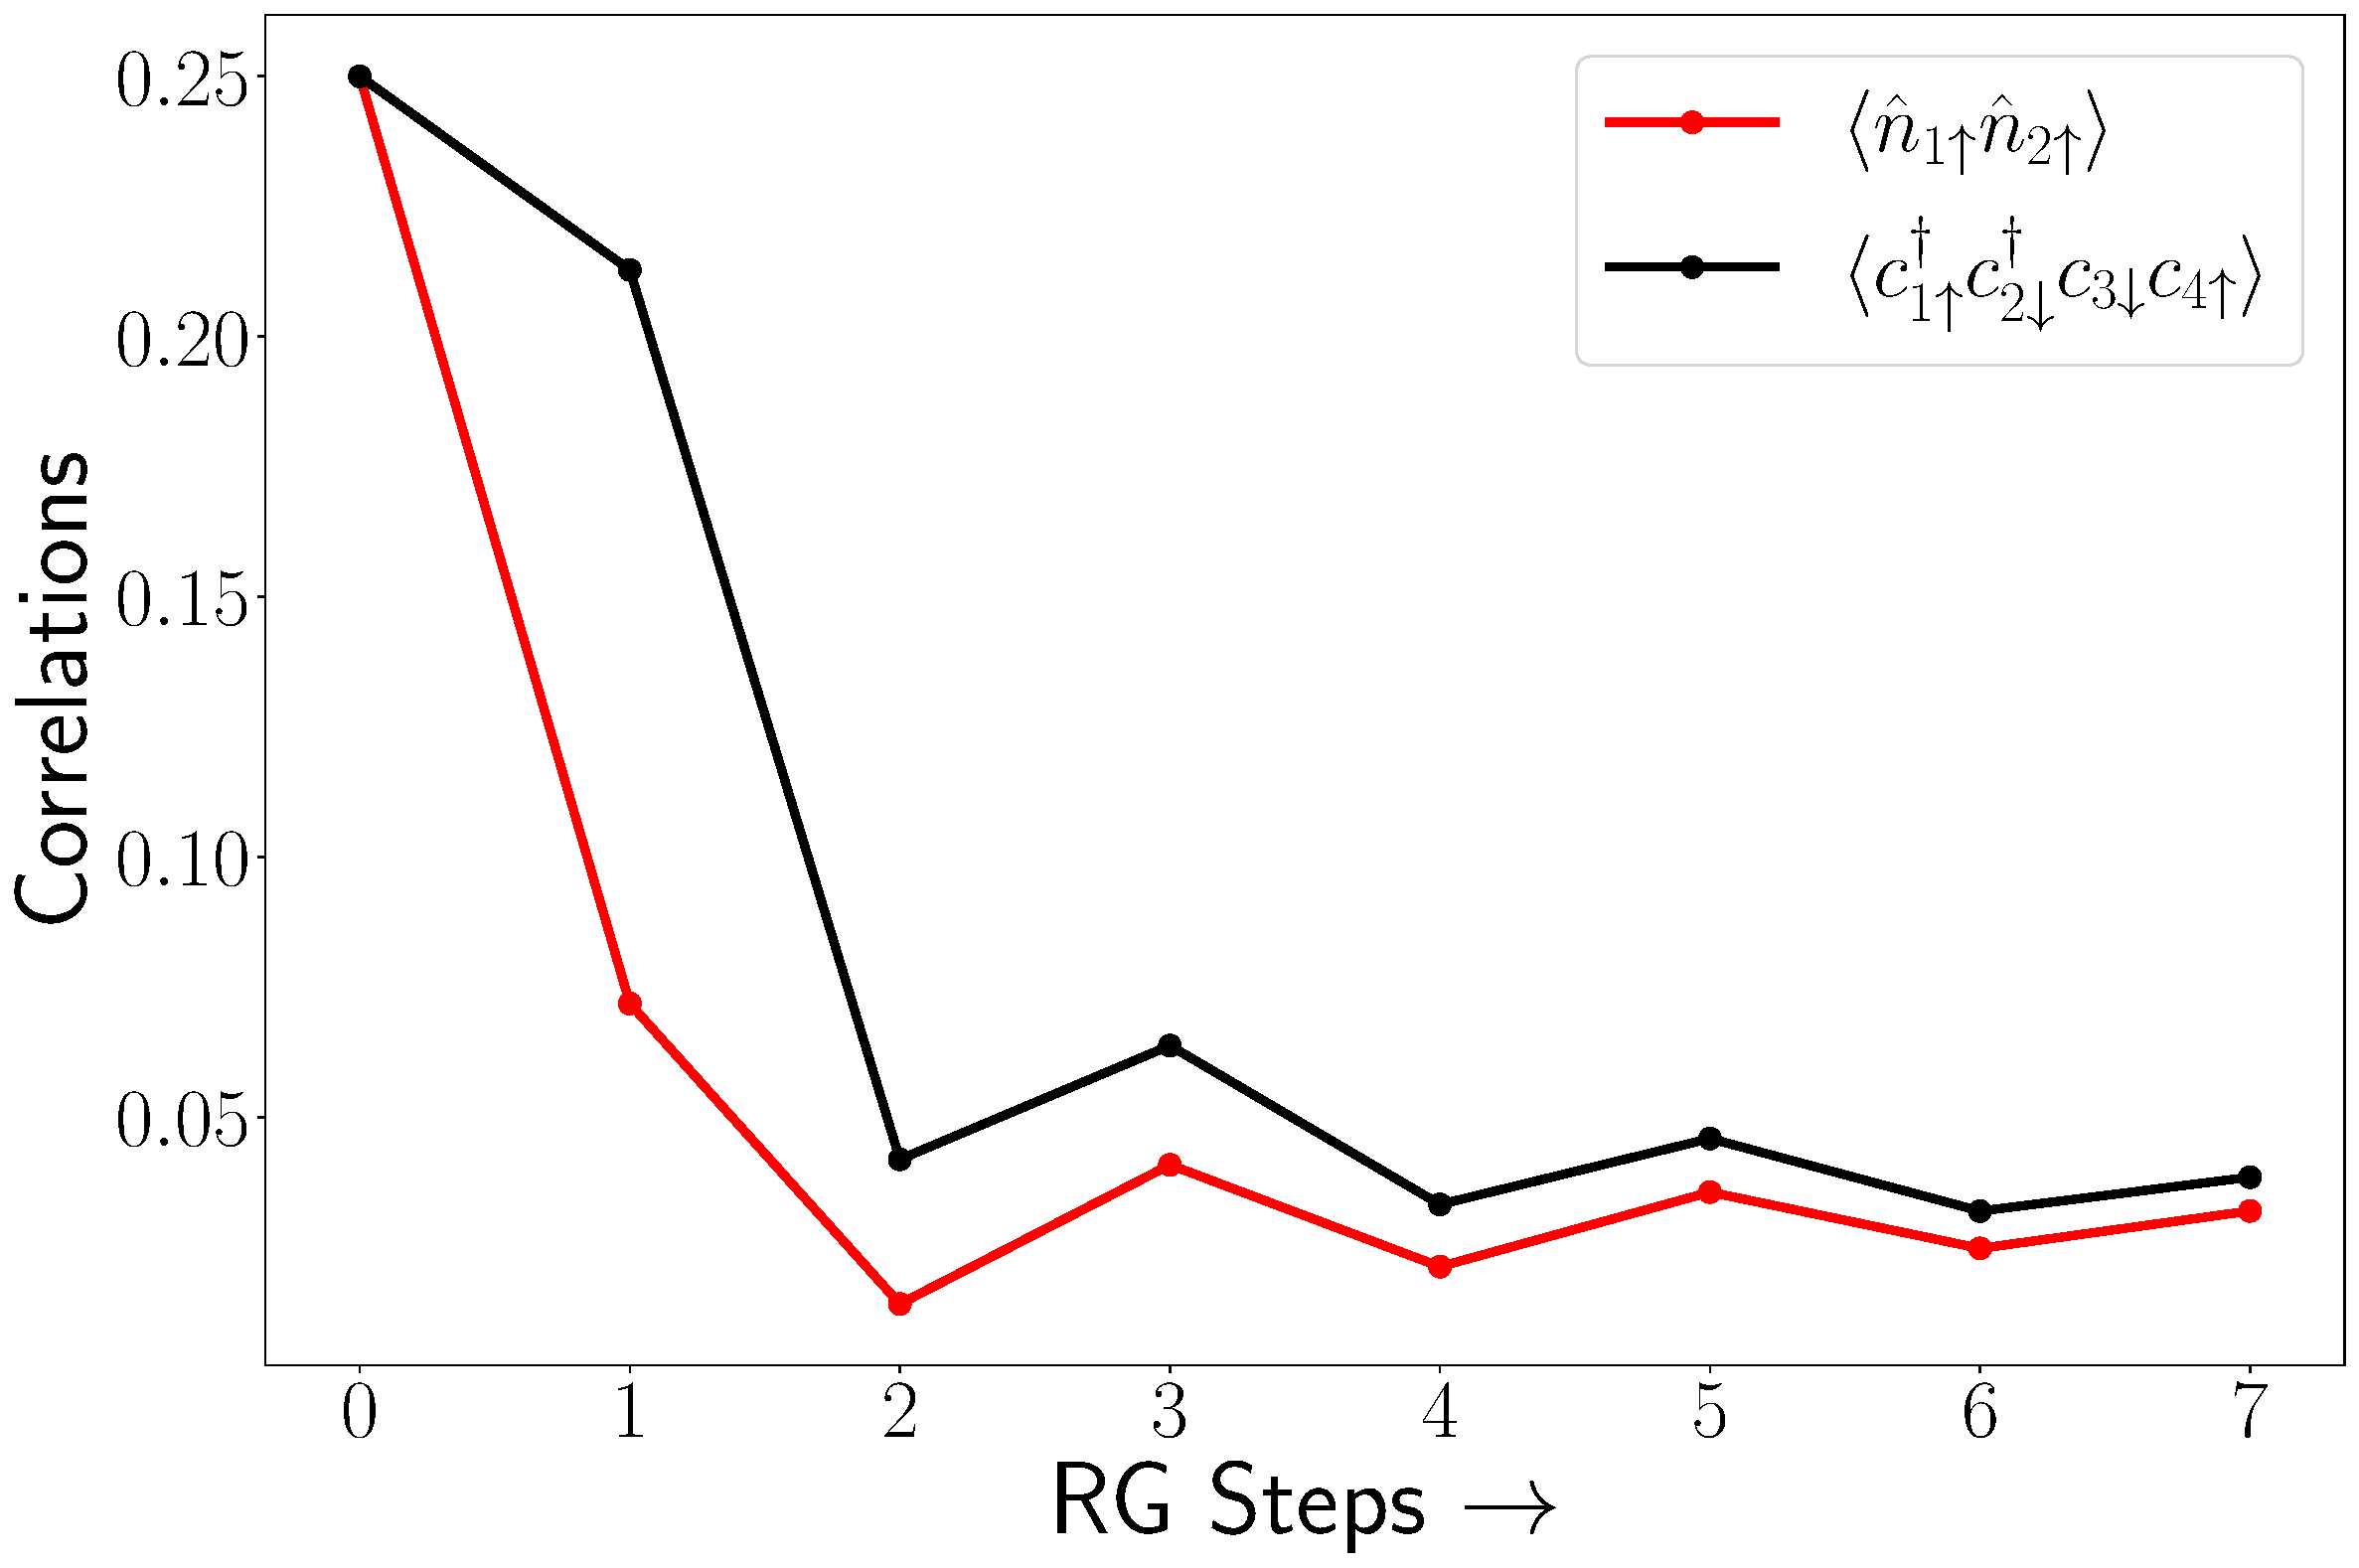
\includegraphics[width=\textwidth]{figures/corrKondo.pdf}
\end{minipage}
}
}

\end{frame}

\section{Discussions \& Conclusions}
\begin{frame}[noframenumbering]{Discussions \& Conclusions}
	\begin{itemize}[<+-|alert@+>]
		\item \focus{Zero-bandwidth model explains the singlet} state and magnetic susceptibility - acts as a zeroth-level Hamiltonian for studying excitations\\[10pt]
		\item Both diagonal and off-diagonal components in Kondo cloud - off-diagonal component is \focus{responsible for screening}\\[10pt]
 		\item Consistent with \focus{growth of entanglement and off-diagonal correlation} near strong-coupling\\[10pt]
 		\item Possible extensions include a similar analysis for Kondo lattice models: should yield \focus{far richer phase diagram}\\[10pt]
	\end{itemize}
\end{frame}

\begin{frame}[noframenumbering]{}

{\hspace*{\fill}\bf \Large That's all. Thank you! \hspace*{\fill}}

\vspace*{\fill}

Anirban Mukherjee thanks the CSIR, Govt. of India and IISER Kolkata for funding through a research fellowship. Abhirup Mukherjee thanks IISER Kolkata for funding through a research fellowship. AM and SL thank JNCASR, Bangalore for hospitality at the inception of this work. SL acknowledges funding from a SERB grant. NSV acknowledges funding from JNCASR and a SERB grant (EMR/2017/005398)

\vspace*{\fill}
\begin{figure}
	\hspace*{\fill}
	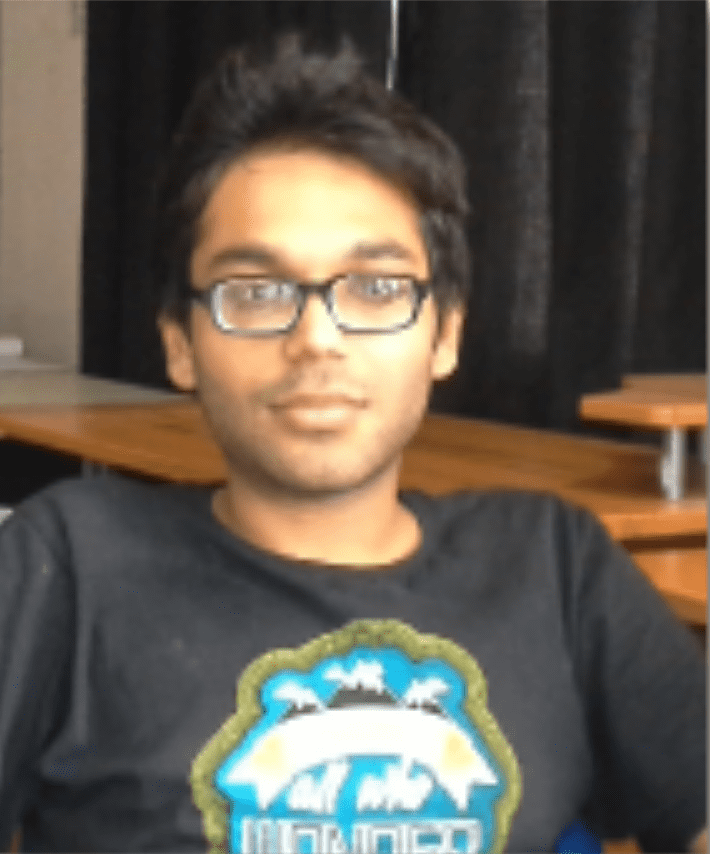
\includegraphics[height=60pt]{figures/am.png}
	\hspace*{\fill}
	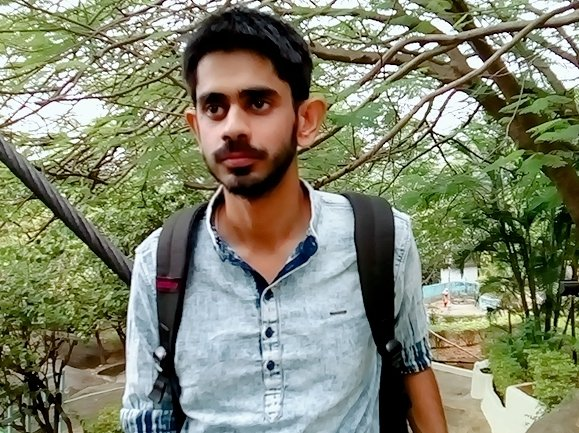
\includegraphics[height=60pt]{figures/dp.jpg}
	\hspace*{\fill}
	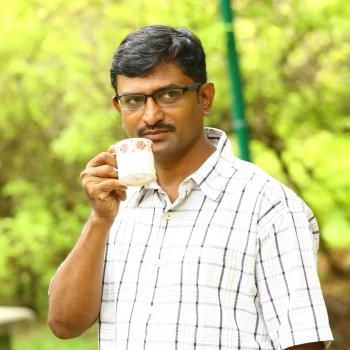
\includegraphics[height=60pt]{figures/ns.jpeg}
	\hspace*{\fill}
	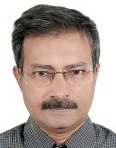
\includegraphics[height=60pt]{figures/arghyat.png}
	\hspace*{\fill}
	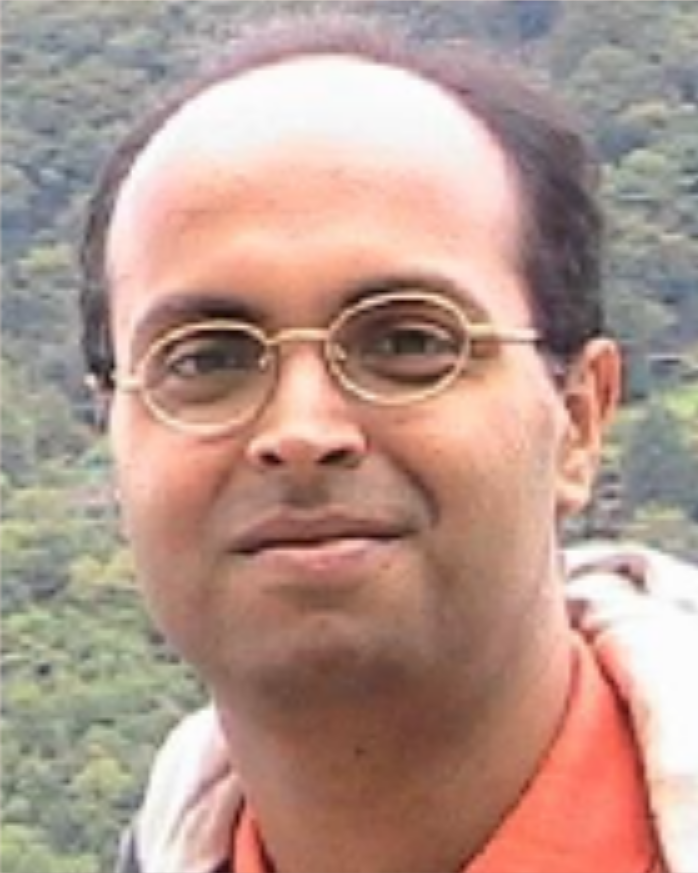
\includegraphics[height=60pt]{figures/slal.jpg}
	\hspace*{\fill}
\end{figure}
\end{frame}

\begin{frame}[noframenumbering,allowframebreaks]{References}
\printbibliography
\end{frame}

\section{Other Results}
\begin{frame}[noframenumbering]{Spectral function}
\begin{minipage}{0.45\textwidth}
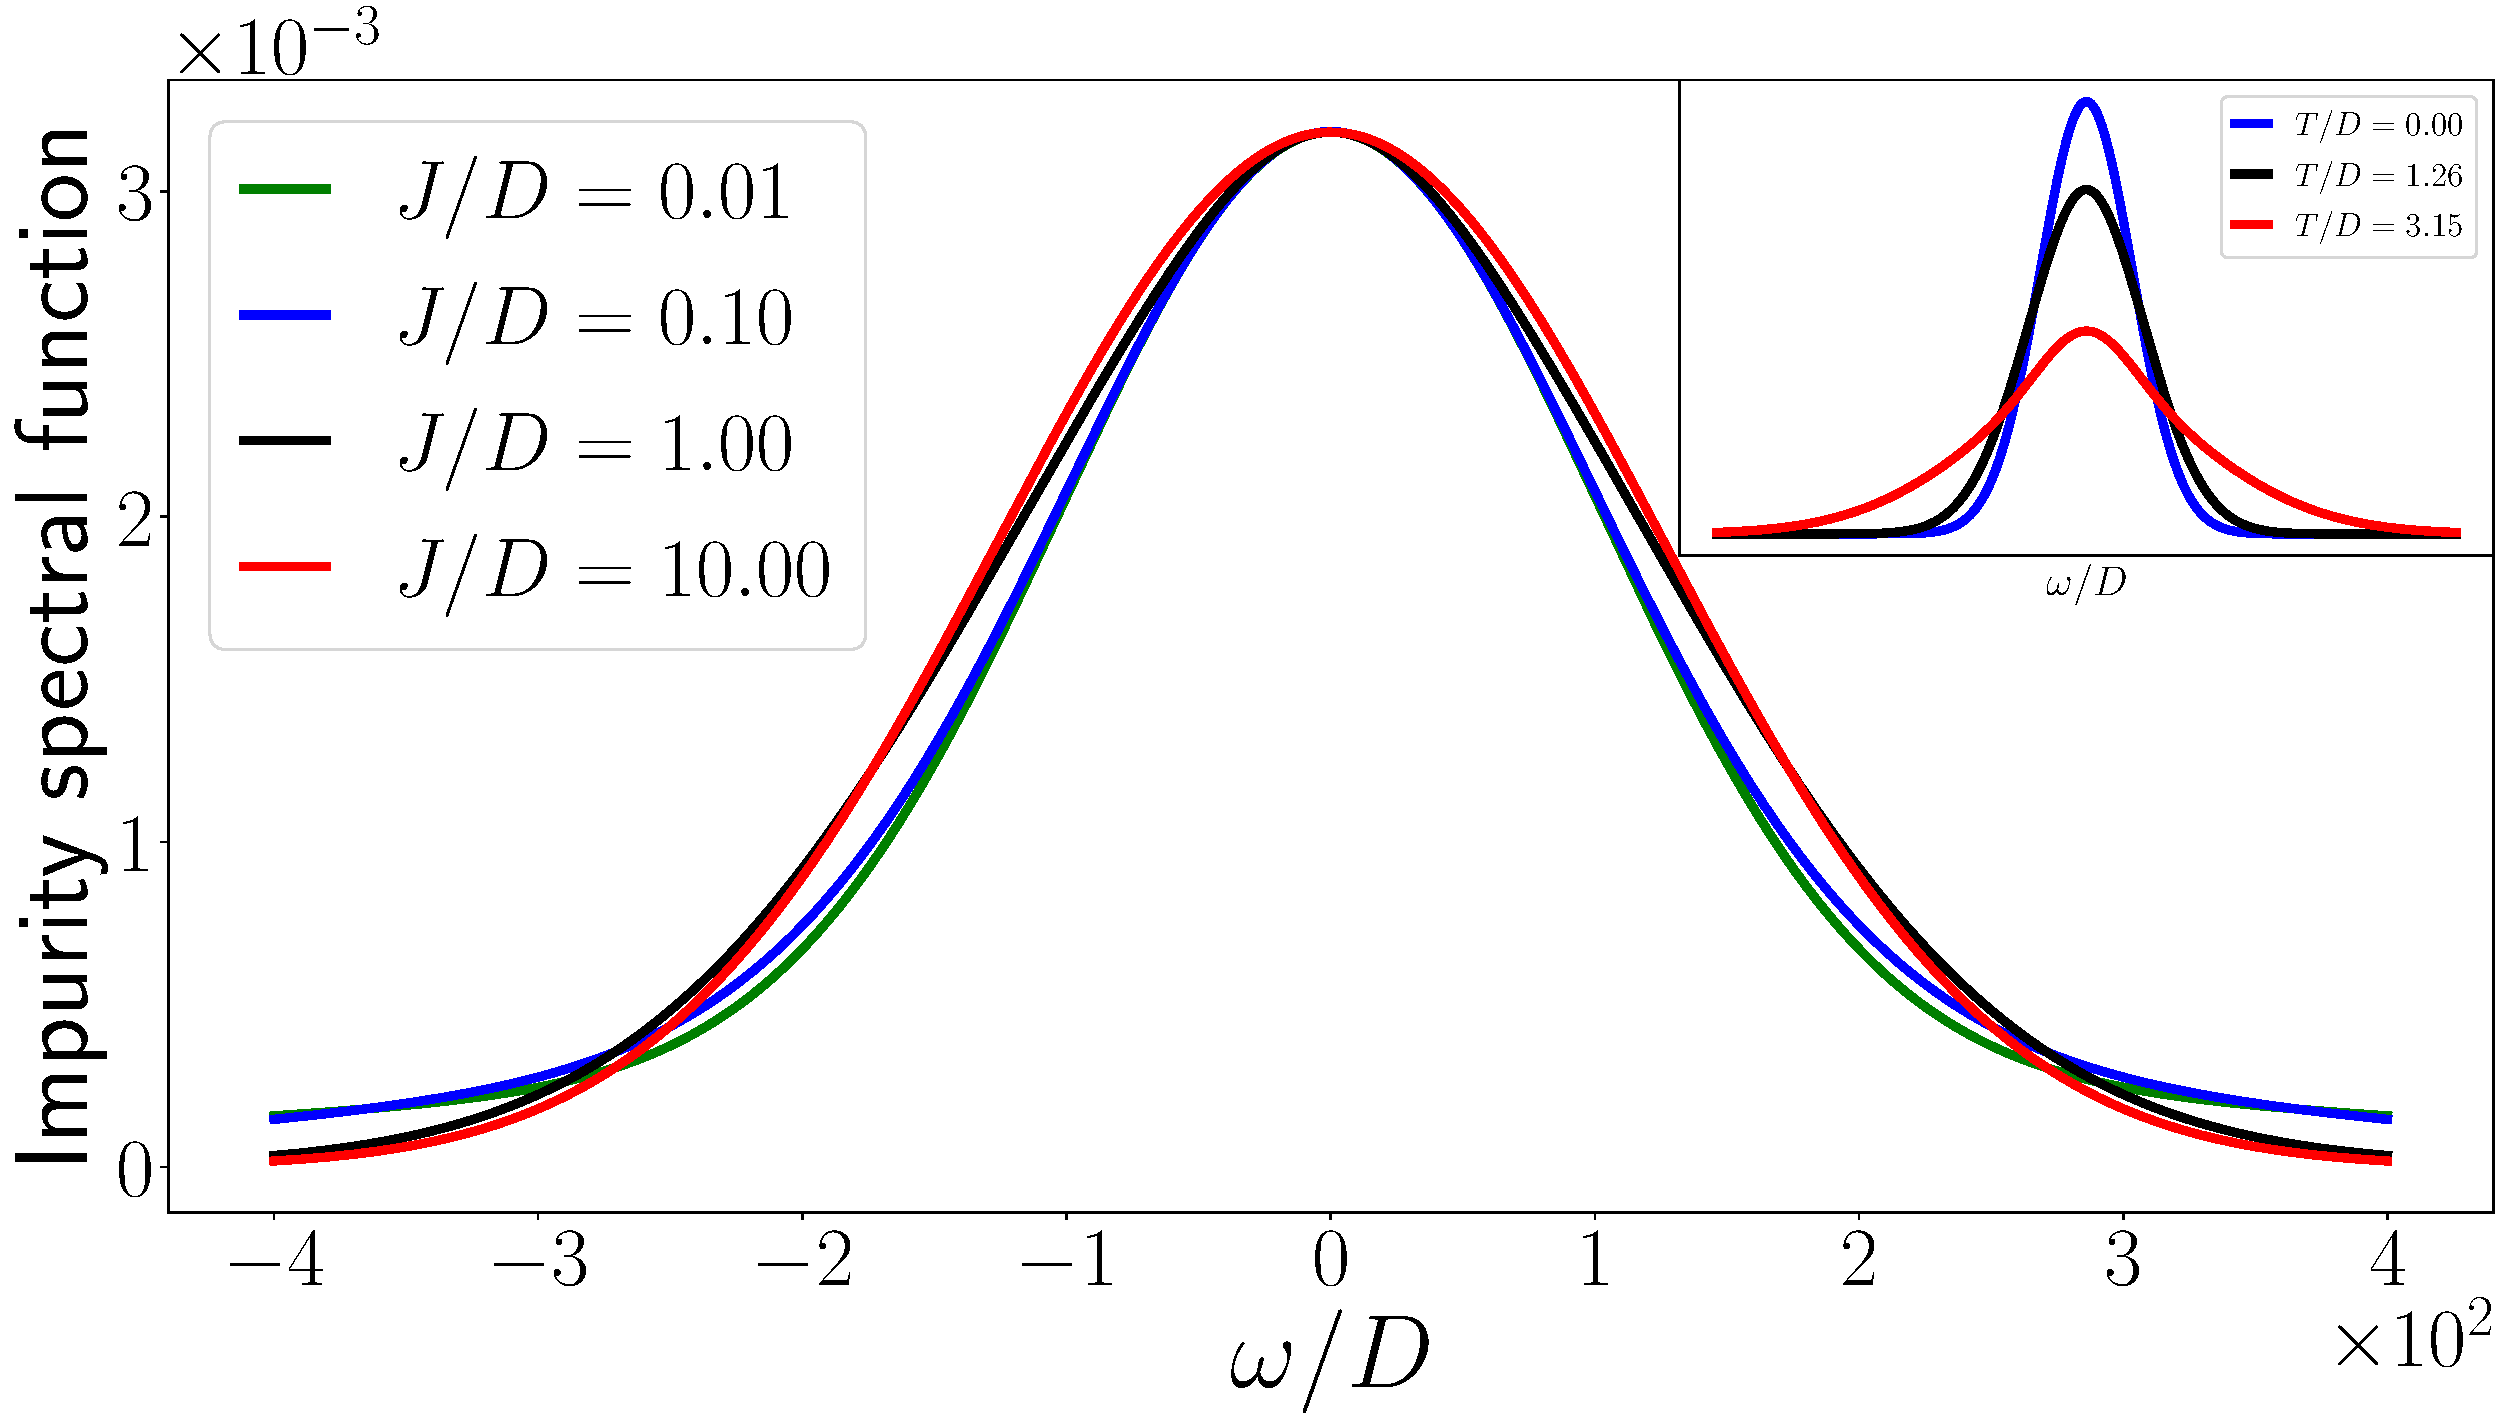
\includegraphics[width=\textwidth]{figures/kondo_spec_func.pdf}
\end{minipage}
\begin{minipage}{0.45\textwidth}
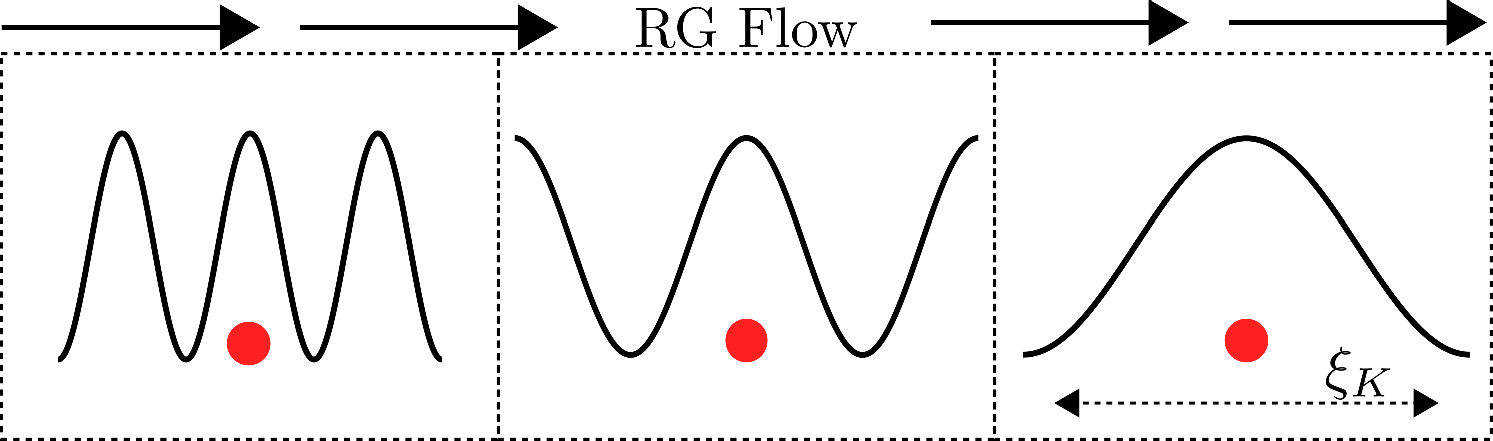
\includegraphics[width=\textwidth]{figures/Kondo_length.pdf}
\end{minipage}
\end{frame}

\begin{frame}[noframenumbering]{\(\chi \times T\) and thermal entropy via zero-bandwidth model}
	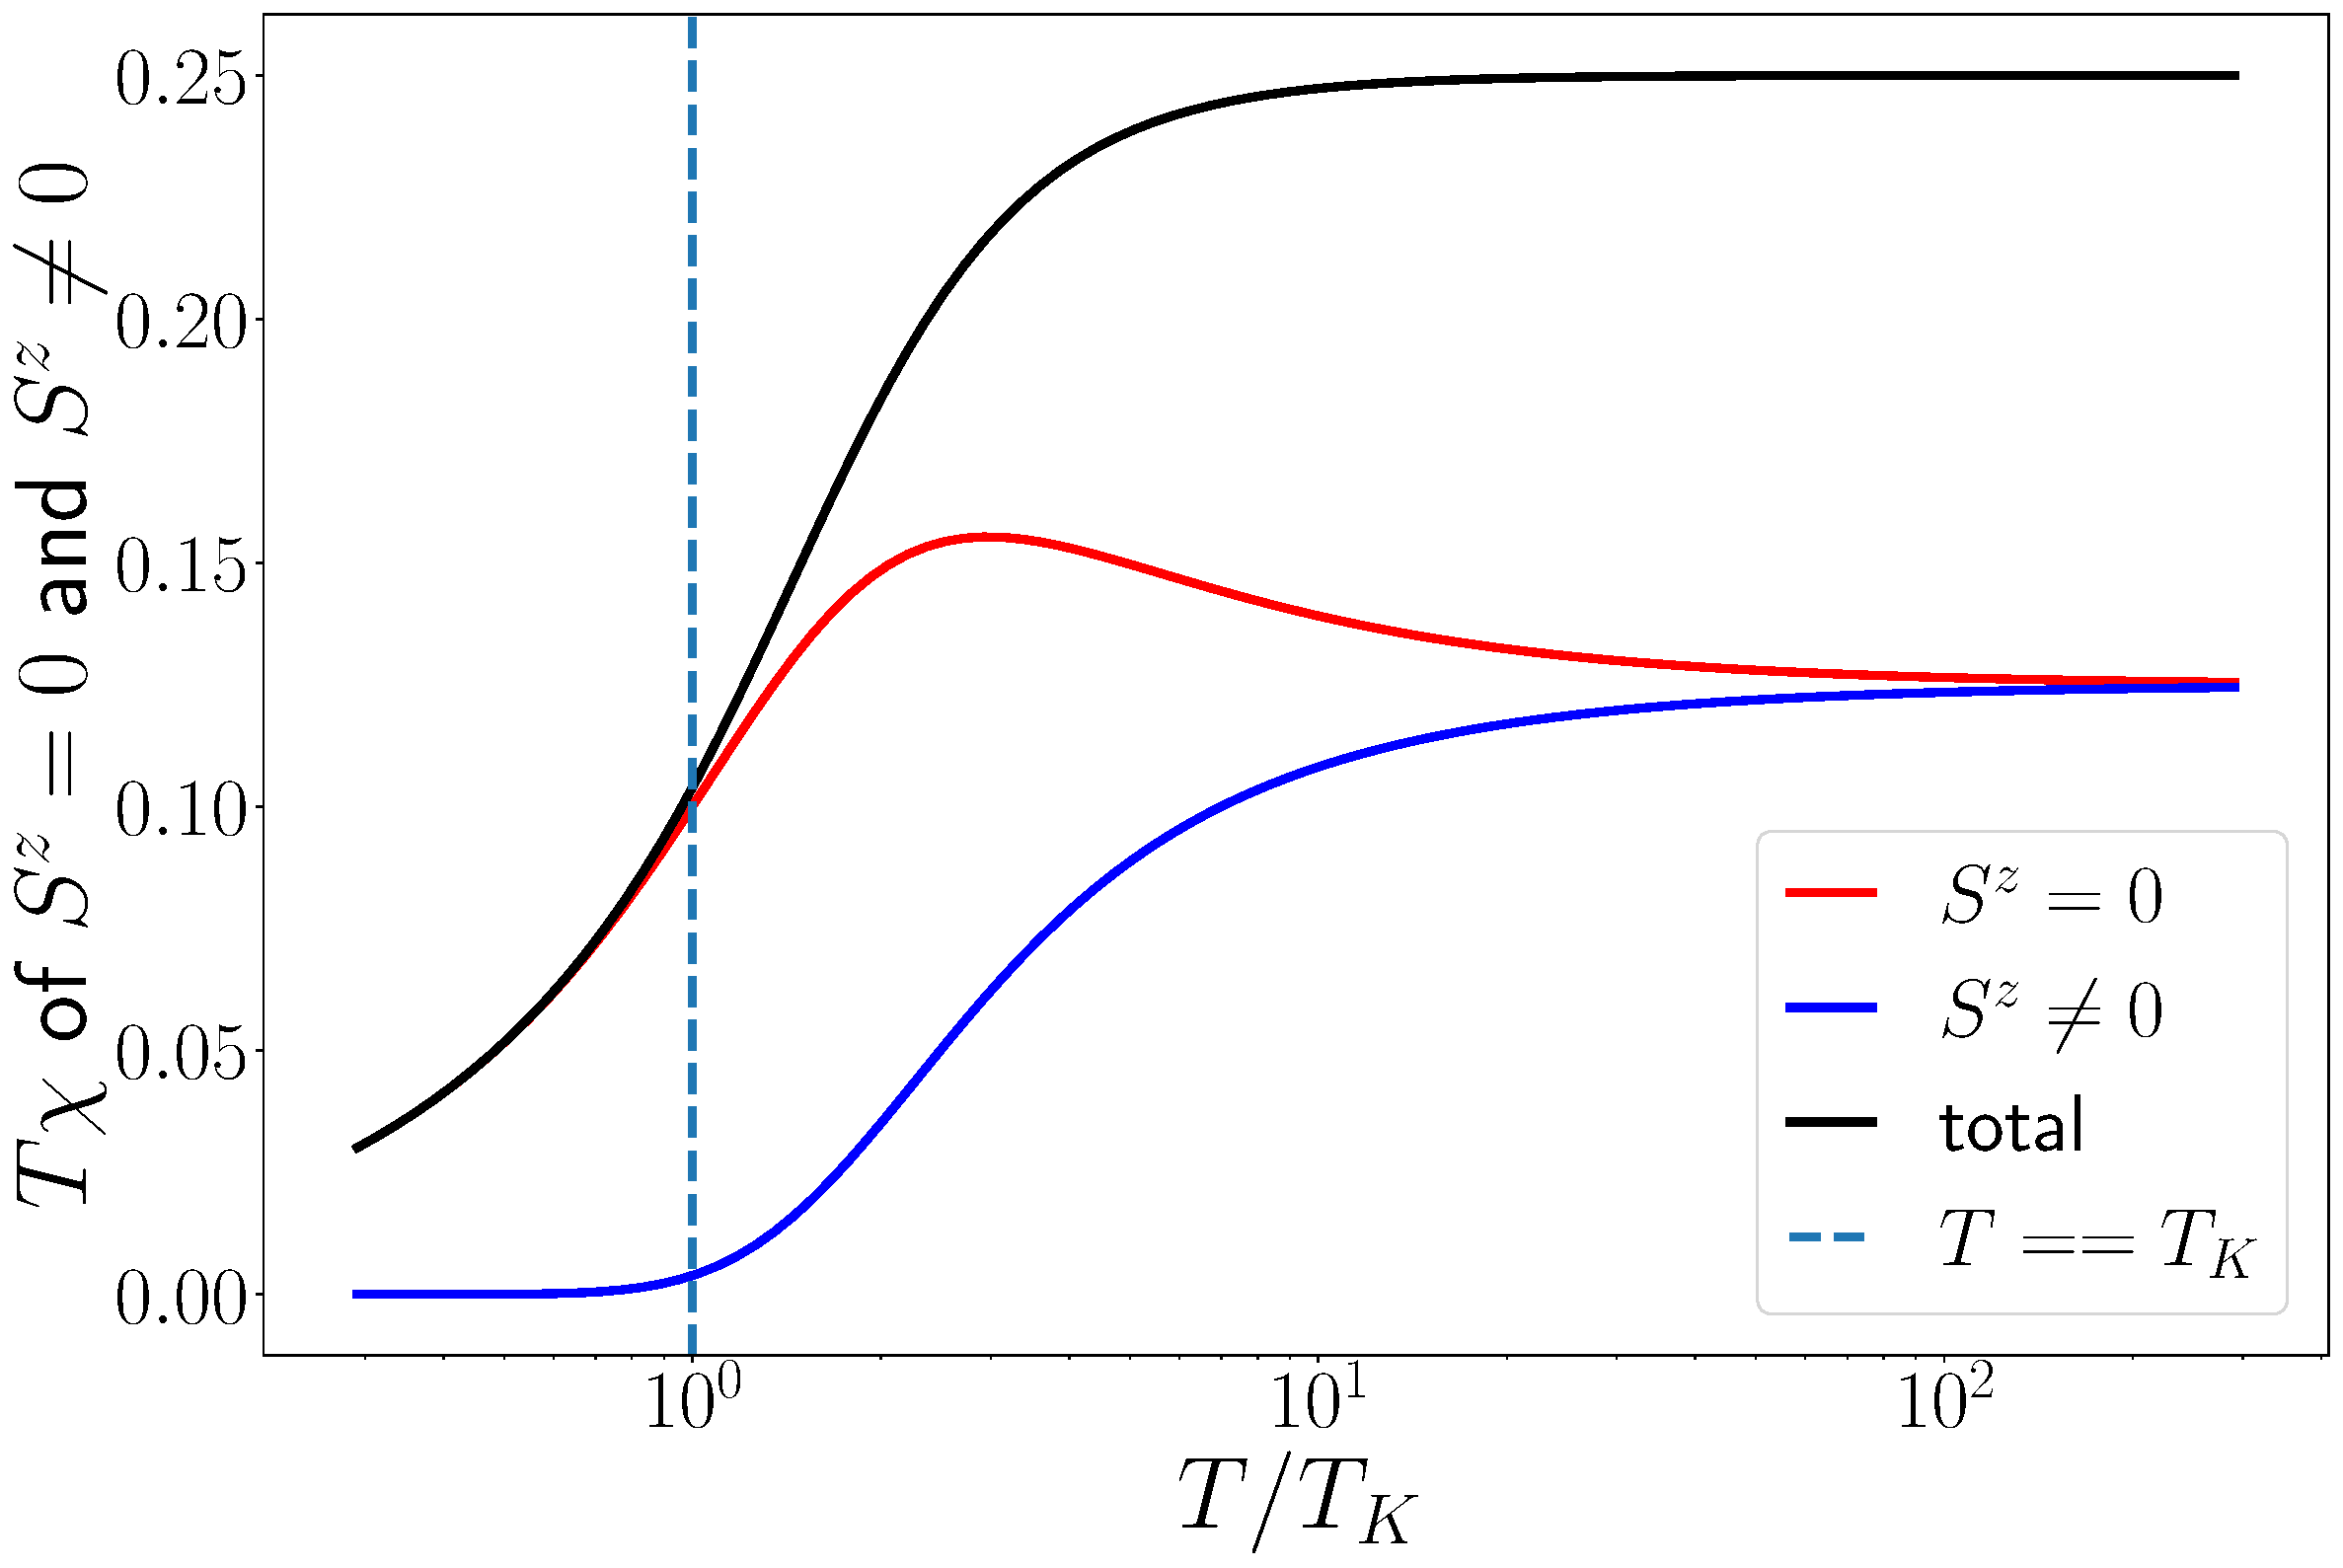
\includegraphics[width=0.45\textwidth]{figures/chi_times_T_parts.pdf}
	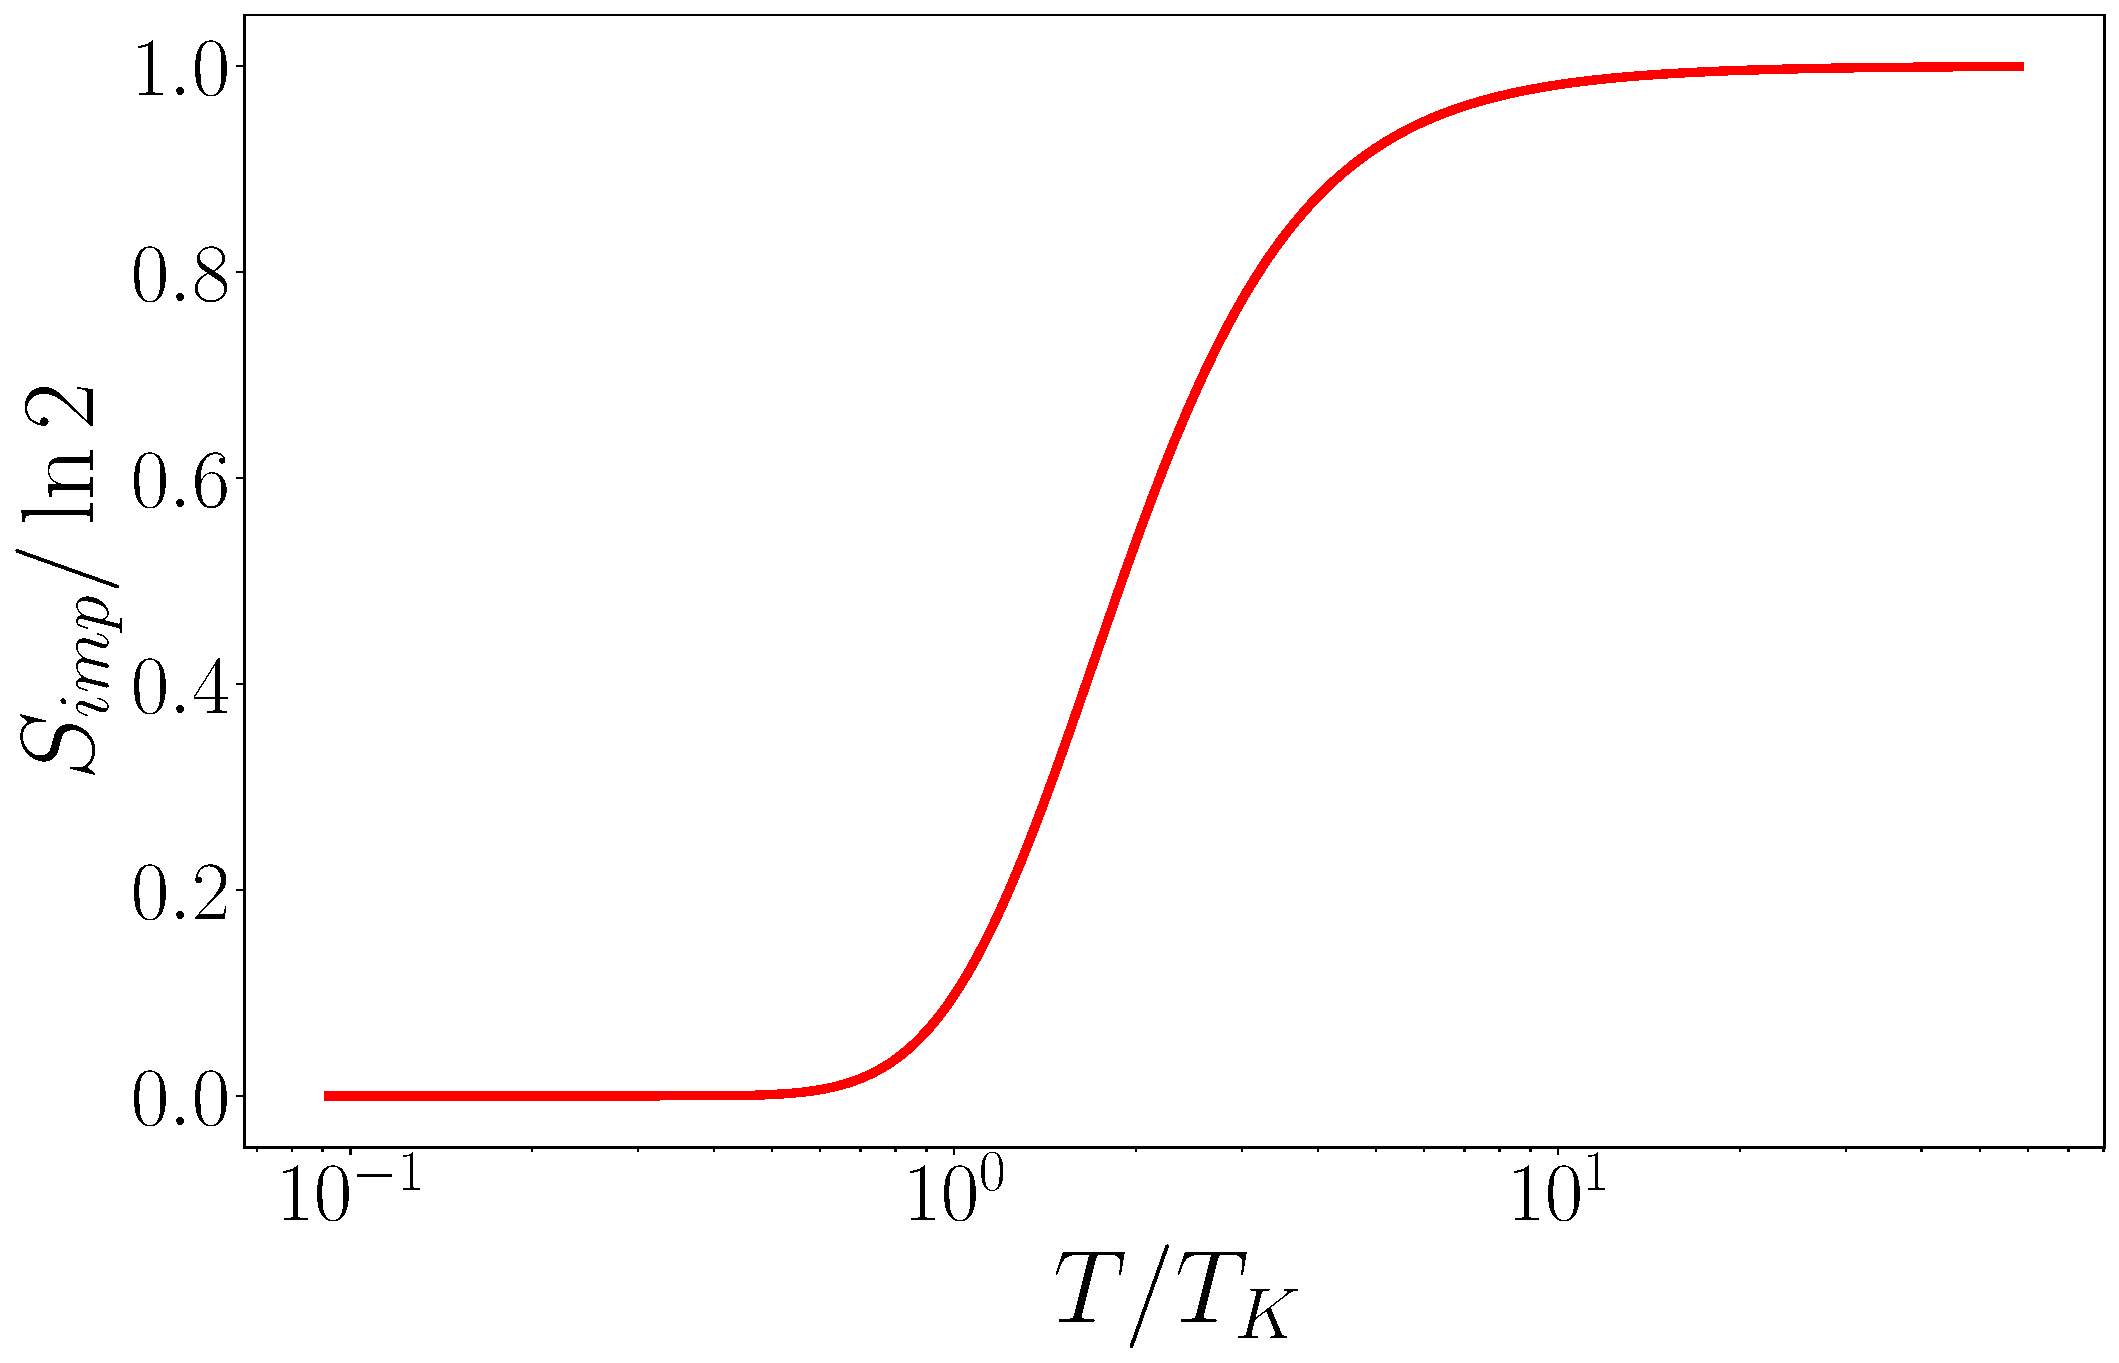
\includegraphics[width=0.45\textwidth]{figures/entropy_therm.pdf}
\end{frame}
\begin{frame}[noframenumbering]{Mutual Information (Kondo regime of SIAM)}
	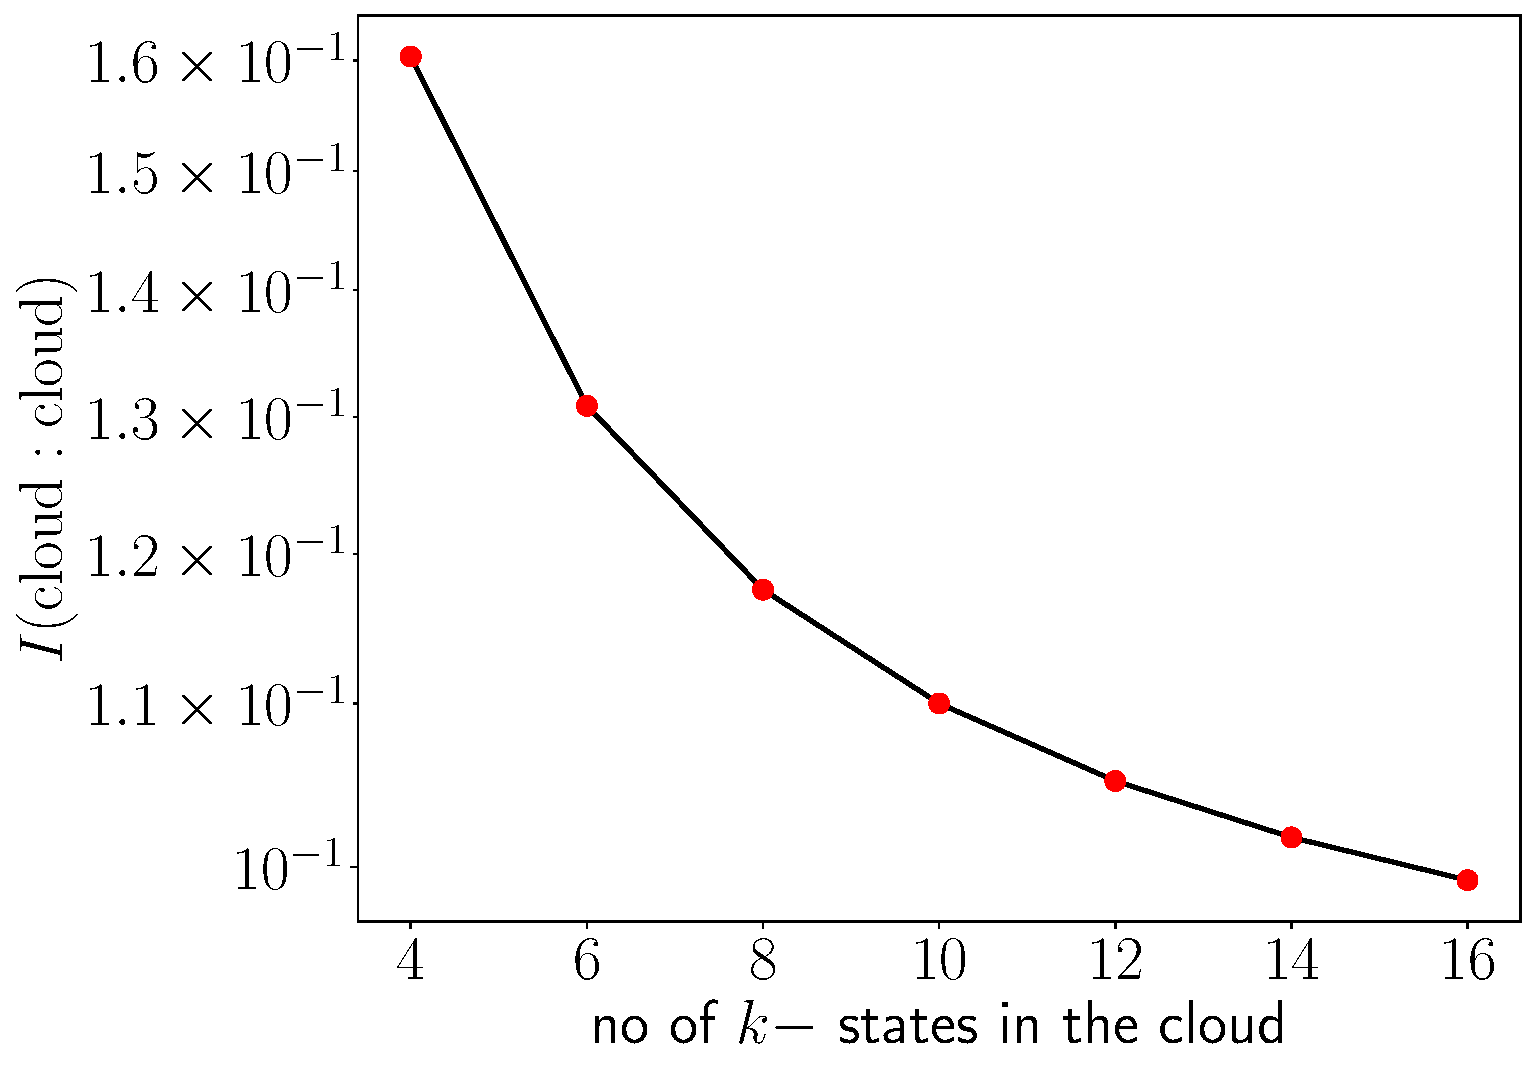
\includegraphics[width=0.45\textwidth]{figures/mut_I_ee.pdf}
	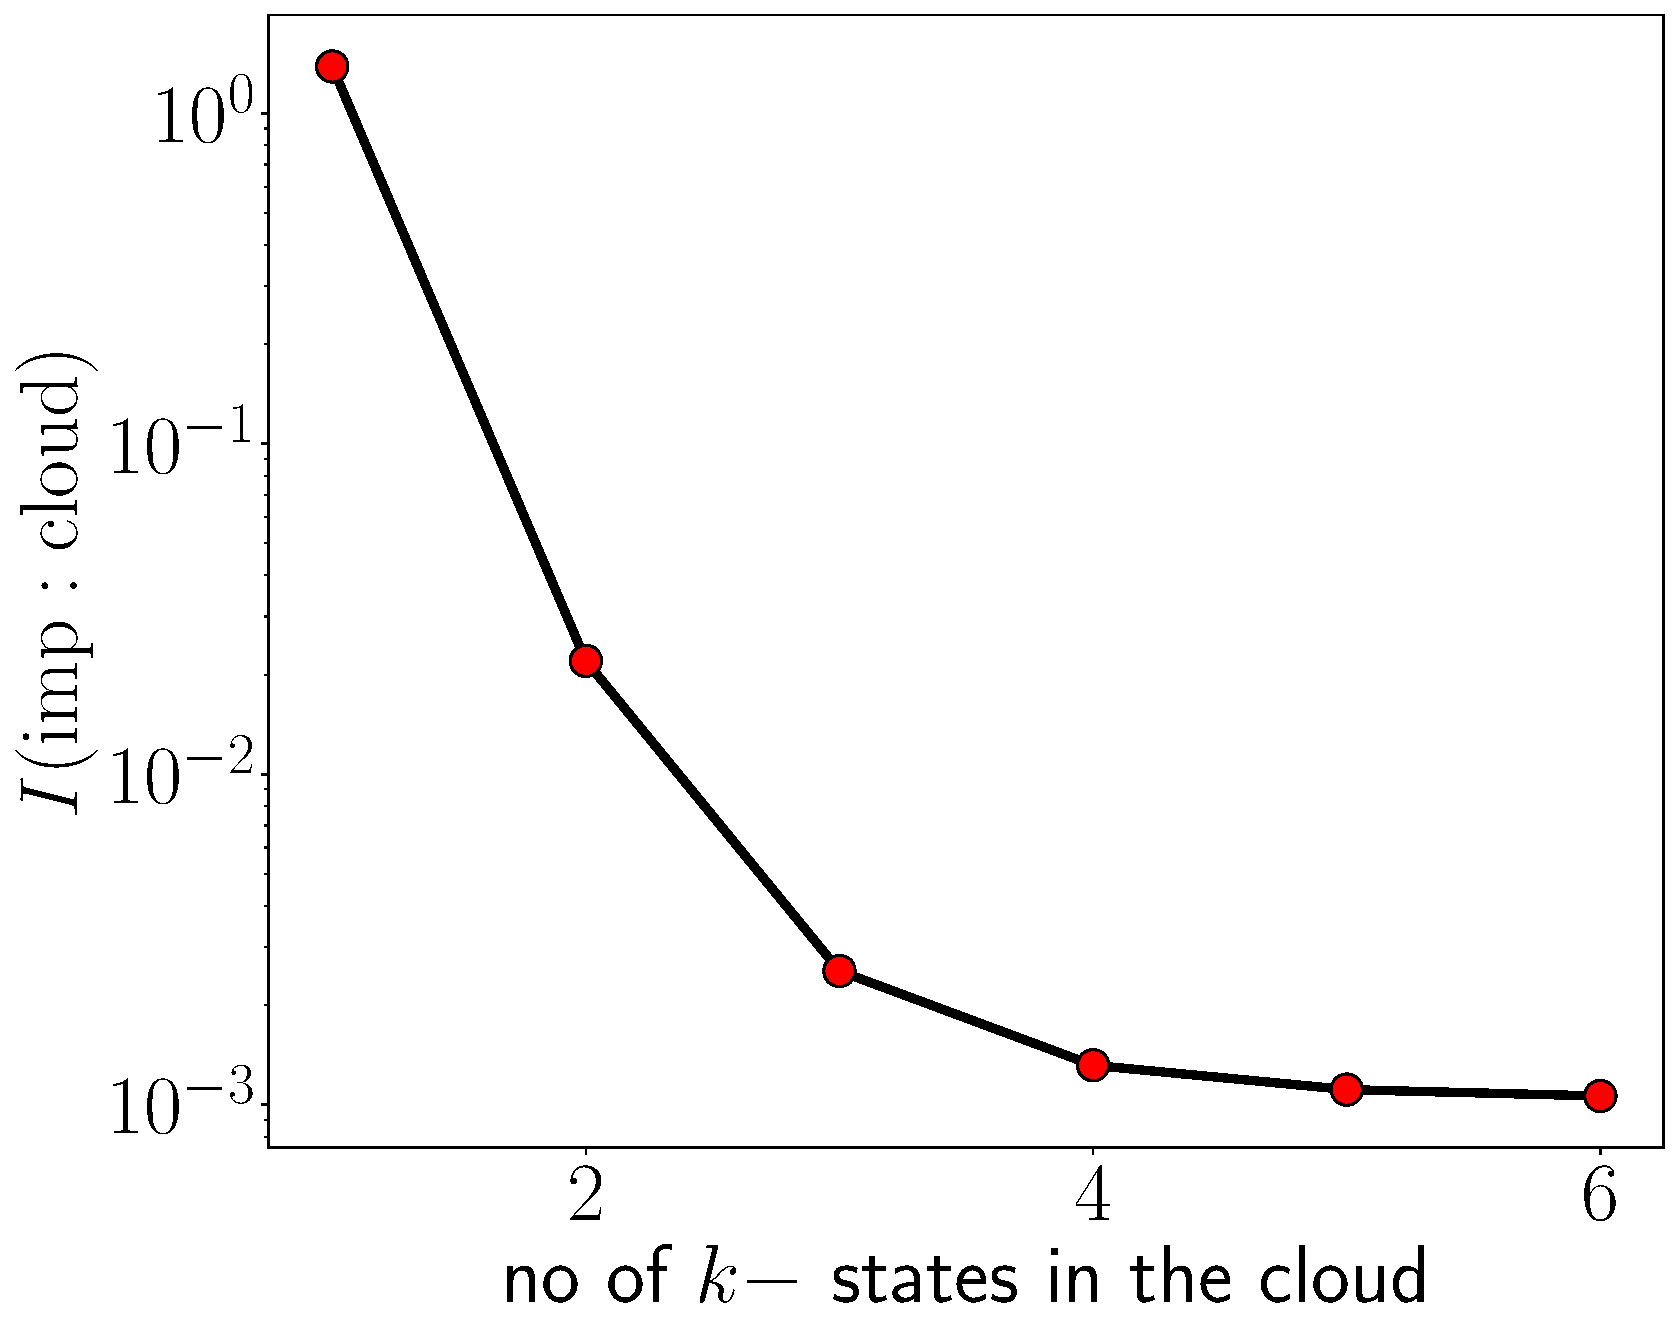
\includegraphics[width=0.45\textwidth]{figures/mut_I_ie.pdf}
\end{frame}
\begin{frame}[noframenumbering]{Many-body correlation (Kondo regime of SIAM)}
	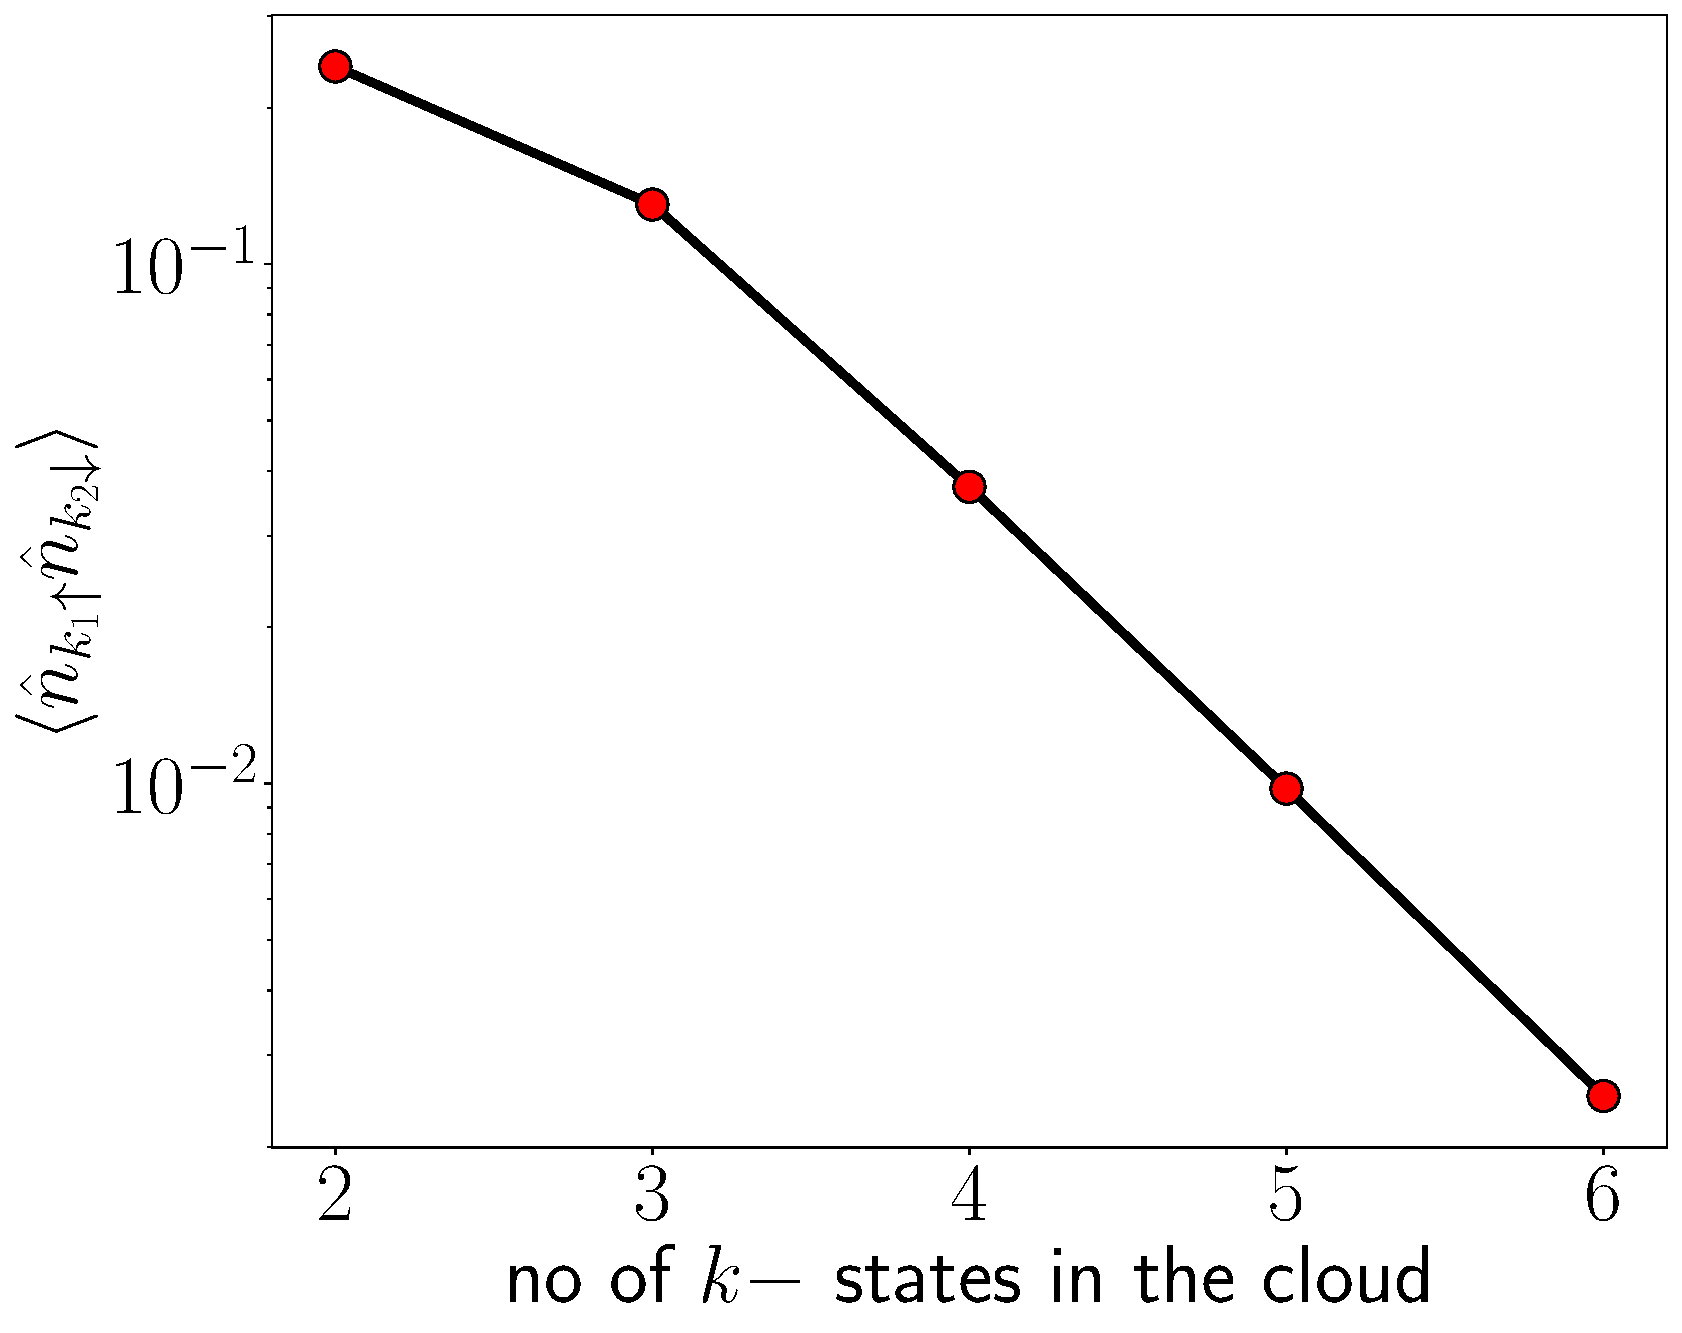
\includegraphics[width=0.45\textwidth]{figures/corr_opp.pdf}
	\includegraphics[width=0.45\textwidth]{figures/corr_od.pdf}
\end{frame}

\begin{frame}[noframenumbering]{Local Fermi liquid excitations}
\head{Effective Hamiltonian in singlet subspace}
\begin{minipage}{0.5\textwidth}
\only<1>{We approximate the dispersion as a \focus{real-space nearest neighbour hopping}:
\[H^* = J^* \vec{S}_d\cdot\vec{s}_< - t\sum_{i\sigma}\left(c^\dagger_{i\sigma}c_{i+1,\sigma} + \text{h.c.}\right)\]
\[t \ll J\]
}
\only<2>{Initially consider \focus{just the first site}. Treat \focus{hopping as perturbation}:
\[\ket{\Psi}^*_0 = \frac{1}{\sqrt 2}\left(\ket{\uparrow,\downarrow} - \ket{\downarrow,\uparrow}\right) \]
\[ V =- t\sum_{\sigma}\left(c^\dagger_{0\sigma}c_{1,\sigma} + \text{h.c.}\right)\]
}
\only<3>{At \focus{fourth order}, effective Hamiltonian is
	\[H^*_\text{eff} = -\frac{16\alpha t^4}{3 {J^*}^3}\mathcal{P}_\text{spin} + \frac{32\alpha t^4}{3 {J^*}^3}\mathcal{P}_\text{charge}\]
\[\mathcal{P}_\text{spin} \longrightarrow \text{projector onto }\hat n_1 = 1\]
\[\mathcal{P}_\text{charge} \longrightarrow \text{projector onto }\hat n_1 \neq 1\]
\begin{itemize}
	\item charge sector  has a \focus{repulsive term}
	\item so, first site harbours a local FL
\end{itemize}
}
\only<4>{On reinstating the \focus{rest of the sites}, the complete effective Hamiltonian is
	\[H^*_\text{eff} = |\mathcal{C}_\text{LFL}|\mathcal{P}_\text{charge} - t\sum_{i>0,\sigma}\left(c^\dagger_{i\sigma}c_{i+1,\sigma} + \text{h.c.}\right)\]
}
\end{minipage}
\hspace*{\fill}
\begin{minipage}{0.4\textwidth}
	\only<1>{\includegraphics[width=0.9\textwidth]{figures/noz_1D.pdf}}
	\only<2>{\includegraphics[width=0.9\textwidth]{figures/noz_1D_approx.pdf}}
	\only<3>{\includegraphics[width=0.9\textwidth]{figures/lattice_eff.pdf}}
	\only<4>{\includegraphics[width=0.9\textwidth]{figures/lattice_eff_full.pdf}}
\end{minipage}
\end{frame}

\end{document}
